%input macros (i.e. write your own macros file called MacroFile1.tex)
%% Personal macros
\newcommand{\JENC}{Jens Enzo Nyby Christensen}
\newcommand{\email}{jens@jensenzo.com}

%% Editing macros
\newcommand{\todo}[1]{\textcolor{red}{@TODO: #1}}

%% Maths macros
\newcommand{\argmin}[1]{\underset{#1}{\mathrm{argmin}}}
\newcommand{\argmax}[1]{\underset{#1}{\mathrm{argmax}}}

%% Functional short-hands and inserts
\newcommand{\PdfPsText}[2]{
  \ifpdf
     #1
  \else
     #2
  \fi
}

\newcommand{\IncludeGraphicsH}[3]{
  \PdfPsText{\includegraphics[height=#2]{#1}}{\includegraphics[bb = #3, height=#2]{#1}}
}

\newcommand{\IncludeGraphicsW}[3]{
  \PdfPsText{\includegraphics[width=#2]{#1}}{\includegraphics[bb = #3, width=#2]{#1}}
}

\newcommand{\InsertFig}[3]{
  \begin{figure}[!htbp]
    \begin{center}
      \leavevmode
      #1
      \caption{#2}
      \label{#3}
    \end{center}
  \end{figure}
}



%%% Local Variables:
%%% mode: latex
%%% TeX-master: "~/Documents/LaTeX/CUEDThesisPSnPDF/thesis"
%%% End:


\documentclass[oneside,12pt]{Classes/CUEDthesisPSnPDF}


\ifpdf
    \pdfinfo { /Title  (Thesis title)
               /Creator (TeX)
               /Producer (pdfTeX)
               /Author (\JENC \email)
               /CreationDate (D:20120606150614)  %format D:YYYYMMDDhhmmss
               /ModDate (D:20030815213532)
               /Subject (Writing a PhD thesis in LaTeX)
               /Keywords (PhD, Thesis)}
    \pdfcatalog { /PageMode (/UseOutlines)
                  /OpenAction (fitbh)  }
\fi

\title{The detection, classification and restoration of impulses in real-time audio}

\ifpdf
  \author{\href{mailto:\email}{\JENC}}
  \collegeordept{\href{http://www.dar.cam.ac.uk}{Darwin College}}
  \university{\href{http://www.cam.ac.uk}{University of Cambridge}}
% insert below the file name that contains the crest in-place of 'UnivShield'
  \crest{
\includegraphics[width=30mm]{UnivShield}}
\else
  \author{\JENS}
  \collegeordept{Department of Engineering}
  \university{University of Cambridge}
% insert below the file name that contains the crest in-place of 'UnivShield'
  \crest{
\includegraphics[bb = 0 0 292 336, width=30mm]{UnivShield}}
\fi
%
% insert below the file name that contains the crest in-place of 'UnivShield'
% \crest{\IncludeGraphicsW{UnivShield}{40mm}{14 14 73 81}}
%
%\renewcommand{\submittedtext}{change the default text here if needed}
\degree{Doctor of Philosophy}
\degreedate{Degree date yet to be decided}

% turn of those nasty overfull and underfull hboxes
\hbadness=10000
\hfuzz=50pt

% Put all the style files you want in the directory StyleFiles and usepackage like this:
\usepackage{StyleFiles/watermark}


\begin{document}

%\language{english}

\renewcommand\baselinestretch{1.2}
\baselineskip=18pt plus1pt

% A page with the abstract on including title and author etc may be
% required to be handed in separately. If this is not so, then comment
% the below 3 lines (between '\begin{abstractseparte}' and
% 'end{abstractseparate}'), normally like a declaration ... needs some more
% work, mind as environment abstracts creates a new page!
% \begin{abstractseparate}
%   
% Thesis Abstract -----------------------------------------------------


%\begin{abstractslong}    %uncommenting this line, gives a different abstract heading
%\begin{abstracts}        %this creates the heading for the abstract page
\begin{thesissummary}
Impact related audio pulses are a frequent, and mostly undesirable, occurrence on many modern integrated devices. This thesis has explored two aspects of these pulses in real-time audio streams. Firstly a functional view of pulses that aimed to localise impact sites of touch events solely based on a single audio stream. This work is framed as a proposed touchscreen interface. Secondly, the pulses were considered noise and a real-time single-channel detection and restoration system was constructed for a telecommunication application.

Results showed that it is possible, using a large aligned ensemble of training pulses and PCA factorisation, to accurately and robustly estimate the origin of impact sites on a device. It was also found that the use of PCA enabled acceptance of a higher degree of variability within individual spots. Results also showed that pulses could successfully be modelled as linear scalings of a combination of components, yielding increased performance. A generalised multi-channel implementation further increased performance of the system. It was also found that the wavelet basis is accurately able to detect transient noise pulses with high temporal accuracy. False detection rates were compared with competing methods on a large corpus of data and the proposed model perform similarly or better. Furthermore it was found that real-time interpolation of missing data was possible directly on the wavelet coefficients. These results were verified with both objective perceptual models, standard error metrics and subjective listening tests.



\end{thesissummary}
%\end{abstracts}
%\end{abstractslong}


% ----------------------------------------------------------------------


%%% Local Variables:
%%% mode: latex
%%% TeX-master: "../thesis"
%%% End:

% \end{abstractseparate}


% Using the watermark package which is in StyleFiles/
% and to remove DRAFT COPY ONLY appearing on the top of all pages comment out below line
\watermark{DRAFT COPY ONLY}


\maketitle

%set the number of sectioning levels that get number and appear in the contents
\setcounter{secnumdepth}{3}
\setcounter{tocdepth}{3}

\frontmatter
% Thesis Dedictation ---------------------------------------------------

\begin{dedication} %this creates the heading for the dedication page

I would like to dedicate this thesis to my loving parents ...

\end{dedication}

% ----------------------------------------------------------------------

%%% Local Variables: 
%%% mode: latex
%%% TeX-master: "../thesis"
%%% End: 

% Thesis Acknowledgements ------------------------------------------------


%\begin{acknowledgementslong} %uncommenting this line, gives a different acknowledgements heading
\begin{acknowledgements}      %this creates the heading for the acknowlegments


And I would like to acknowledge ...


\end{acknowledgements}
%\end{acknowledgmentslong}

% ------------------------------------------------------------------------

%%% Local Variables: 
%%% mode: latex
%%% TeX-master: "../thesis"
%%% End: 


% Thesis Abstract -----------------------------------------------------


%\begin{abstractslong}    %uncommenting this line, gives a different abstract heading
%\begin{abstracts}        %this creates the heading for the abstract page
\begin{thesissummary}
Impact related audio pulses are a frequent, and mostly undesirable, occurrence on many modern integrated devices. This thesis has explored two aspects of these pulses in real-time audio streams. Firstly a functional view of pulses that aimed to localise impact sites of touch events solely based on a single audio stream. This work is framed as a proposed touchscreen interface. Secondly, the pulses were considered noise and a real-time single-channel detection and restoration system was constructed for a telecommunication application.

Results showed that it is possible, using a large aligned ensemble of training pulses and PCA factorisation, to accurately and robustly estimate the origin of impact sites on a device. It was also found that the use of PCA enabled acceptance of a higher degree of variability within individual spots. Results also showed that pulses could successfully be modelled as linear scalings of a combination of components, yielding increased performance. A generalised multi-channel implementation further increased performance of the system. It was also found that the wavelet basis is accurately able to detect transient noise pulses with high temporal accuracy. False detection rates were compared with competing methods on a large corpus of data and the proposed model perform similarly or better. Furthermore it was found that real-time interpolation of missing data was possible directly on the wavelet coefficients. These results were verified with both objective perceptual models, standard error metrics and subjective listening tests.



\end{thesissummary}
%\end{abstracts}
%\end{abstractslong}


% ----------------------------------------------------------------------


%%% Local Variables:
%%% mode: latex
%%% TeX-master: "../thesis"
%%% End:


\tableofcontents
\listoffigures
\printnomenclature  %% Print the nomenclature
\addcontentsline{toc}{chapter}{Nomenclature}

\mainmatter

%%% Thesis Introduction --------------------------------------------------
\chapter{Introduction}\label{ch:Introduction}
\ifpdf
    \graphicspath{{Introduction/IntroductionFigs/PNG/}{Introduction/IntroductionFigs/PDF/}{Introduction/IntroductionFigs/}}
\else
    \graphicspath{{Introduction/IntroductionFigs/EPS/}{Introduction/IntroductionFigs/}}
\fi

\section{Problem overview}
Transient pulses in an audio stream originating from the physical interaction with a device, are a common feature of modern integrated devices. Microphones are typically incorporated into laptop computers, mobile phones and tablets due to their low price and relatively high utility in relation to single or multi-channel audio recordings or for noise or echo-cancellation applications. The primary function of the embedded microphones is typically to pick up external sounds (external to the device), but as a consequence of the mechanical construction microphones tend to pick up physical interactions with the device as well. In devices with embedded keyboards typing will often produce clearly audible transient pulses in the audio stream, e.g. a conference call, which may be considered a nuisance and even cause a loss of intelligibility. Even interactions via non-physical keys, e.g. touchscreens, will produce a clearly audio pulse in the audio stream of a device. While these audible pulses would be considered a nuisance in the context of a conference call, it is possible that they could provide additional information about the origin of touch interactions in others.

\section{Aims and objectives}
The work presented here will consider two aspects of impact related audio pulses. Firstly the pulses will be considered from a functional perspective as a means for localising impacts, and secondly the pulses will be considered as an annoyance or deleterious effect in the form of noise. It is noted that these two perspectives are not necessarily mutually exclusive, i.e. one might wish to both classify and then remove such a transient.

\subsection{Acoustic pulse recognition (APR)}
\emph{Is it possible to accurately infer the origin of a device-interaction solely based on the audible pulse generated from the interaction?}
This question will be considered primarily from the perspective of a single-channel input and will focus on methods that are computationally realisable in a real-time scenario. The problem will be framed as a touchscreen implementation and will be referred to as acoustic pulse recognition (APR). The performance of the methods developed will be compared and contrasted and various practical concerns associated with the particular application will be discussed. An extension of the application will seek to generalise the application to multiple channels.

An example of a pulse associated with the interaction with a device is shown in Figure~\ref{fig:singleSampleTap.png}. This pulses is recorded from a standard mobile phone (more details in section~\ref{sec:APRsystem}), and the majority of the pulses has decayed after approximately 7 ms.

\begin{figure}
  \begin{center}
    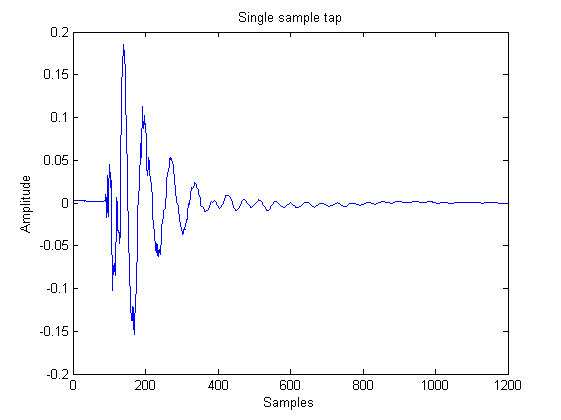
\includegraphics[width=110mm]{singleSampleTap.png}
    \caption{A sample pulse from a mobile phone. Sampled at 44.1 kHz.}\label{fig:singleSampleTap.png}
  \end{center}
\end{figure}

A successful application of a classification algorithm relies on the similarity of pulses from identical impact sites and dissimilarity from those from other sites. Figure~\ref{fig:twotwoSampleTap.png} shows an example of four pulses: two from one spot (blue) and two from a different spot (red). It is clearly seen in Figure~\ref{fig:twotwoSampleTap.png} that while the blue pulses are nearly identical their waveforms are vastly different to that of the red pulses. This observation is, as noted, integral to a successful classification algorithm based on this data. In this example all pulse-onsets have been aligned to the same point.

\begin{figure}
  \begin{center}
    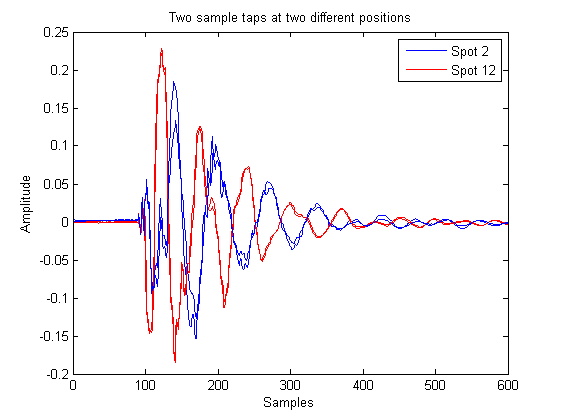
\includegraphics[width=110mm]{twotwoSampleTap.png}
    \caption{Two sets of two sample pulses recorded a two different spots on the mobile phone. Sampled at 44.1 kHz.}\label{fig:twotwoSampleTap.png}
  \end{center}
\end{figure}

While Figure~\ref{fig:twotwoSampleTap.png} shows data obtained in an ideal scenario, pulses will vary greatly depending on factors such as temperature, how the device is suspended and with what it is impacted. The work undertaken in chapters~\ref{ch:APR} and~\ref{ch:MultichannelAPR} will seek to apply this classification algorithm as a real world touch surface application.

% Summary of literature
%A range of applications have been proposed that utilise multiple microphones to implement a touchscreen interface\cite{US8174547}\cite{US8233353}\cite{TouchSystems2006}\cite{US7411581}\cite{WO2006108443}. The functional elements of these methods all rely on their being multiple sources and so the single-channel implementation of the APR system is radically different and should therefore be considered a significant contribution. Not only does the single-channel implementation of the APR system allow for lower hardware cost for integration, it also enables post-hoc integration in system without multiple accessible microphones which currently still is the majority of devices. Work presented in chapter~\ref{ch:APR} is also presented in \cite{Christensen2011} and \cite{US20110316784}.

\subsection{Keyboard stroke removal}
\emph{Is it possible to remove or reduce the effect of transient noise pulses, in particular keyboard stroke noise, on a real-time single channel audio stream for teleconferencing applications?}
This question will again be considered in the context of a realistic teleconferencing scenario. The implementation will be limited by the practical constraints of the webRTC platform and feature a sampling frequency of 16 kHz and buffers of 256 samples with 96 samples of overlap between buffers, leaving 10 ms of new data per buffer. In addition the system needs to be applicable in a real-time scenario setting limits to the computational requirements of the system. The system should be unsupervised, require no training, work on, and remove, a multitude of noise pulses while letting speech signals through unaffected. The system being developed can roughly be divided into two separate parts: a detection stage and a restoration stage. It is the aim to detect pulses reliably while embedded in speech segments, accurately in time and with as few false detections as possible. Restorations of the detected pulses should aim to decrease the nuisance associated with the noise pulses and restored and interpolated segments should be unobtrusive and preferably unnoticeable.

The primary focus of this noise removal algorithm are the noise pulses associated with keyboard typing strokes. As with the more general pulses associated with the classification application the keyboard stroke pulses vary greatly with a range of factors but more importantly they vary between devices. This is a particular issue given that the algorithm specifications requires the algorithm to be unsupervised and will therefore not able to learn the particular signature of keystrokes on a particular device.

Figure~\ref{fig:KeyboardStrokeSlowIntro.pdf} shows an example of the waveform from a single slowly typed keystroke. This single keyboard stroke is noticeably comprised of two individual pulses, where the initial sharply rising pulse is associated with the physical action of the mechanical key being pressed and the secondary lower amplitude pulse nearly 200 ms after the initial pulse is associated with the lifting of the finger from the button. This delay between the two pulses is what defines this keyboard stroke as \emph{slow}, whereas faster typing can leave gaps much shorter. It is also noted that there is a significant slowly decaying low frequency component associated with each individual pulse.

\begin{figure}
  \begin{center}
    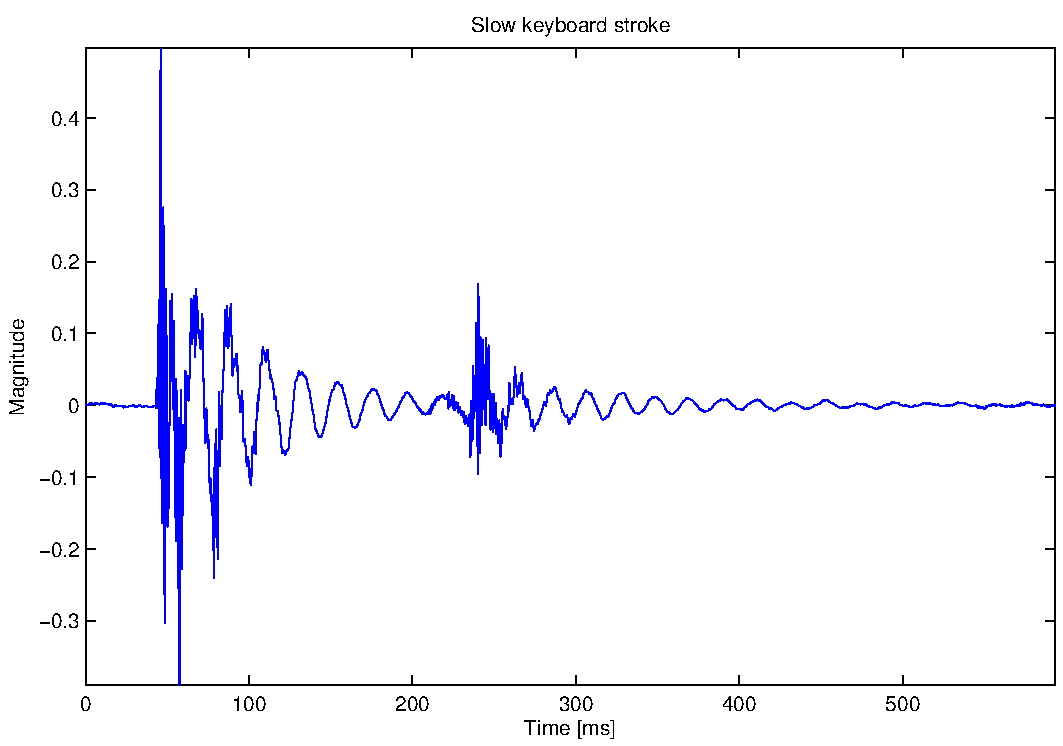
\includegraphics[width=110mm]{KeyboardStrokeSlowIntro.pdf}
    \caption{A sample keystroke sampled at 44.1 kHz.}\label{fig:KeyboardStrokeSlowIntro.pdf}
  \end{center}
\end{figure}

Figure~\ref{fig:shortFastSeq.png} shows the keyboard strokes in the context of a short rapidly typed 5 stroke sequence. The lift-pulses can be seen to appear right before (approximately 10 ms) the second, third and fourth stroke whereas the rest if the lift-pulses are more delayed. It is also noted that while these four primary keystroke-pulses are part of the same sequence they are visually dissimilar. It is also noted that the first stroke clearly shows two distinct pulses in the waveform while an audible evaluation only reveals a single pulse. It is clear that pulses arising from real life typing is extremely varied with only few common features one of which is an initial clear sudden rise noted in the signal amplitude.

\begin{figure}
  \begin{center}
    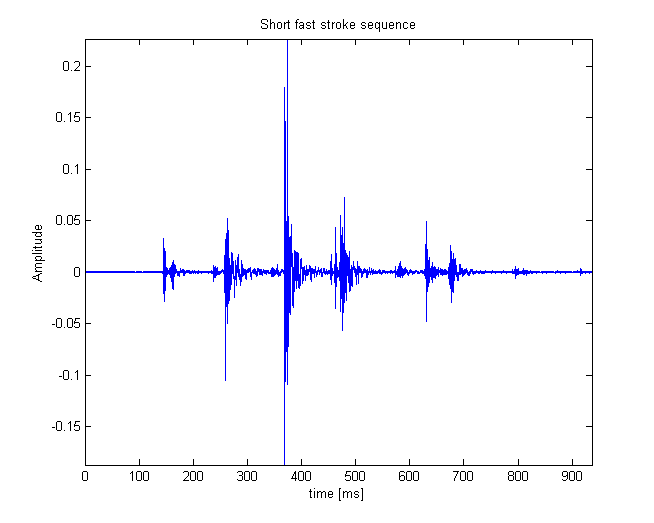
\includegraphics[width=110mm]{shortFastSeq.png}
    \caption{A quickly typed sequence of 5 keyboard strokes sampled at 44.1 kHz.}\label{fig:shortFastSeq.png}
  \end{center}
\end{figure}

Figure~\ref{fig:shortFastSeqSpec.png} shows a spectrogram of the typing sequence displayed in Figure~\ref{fig:shortFastSeq.png}. It is noted that all pulses exhibit a short sudden burst of energy across the spectrum. Even the lift-pulses exhibit this characteristic at a lower level. With each pulses is also a clearly identifiable burst of low frequency energy, in the range of human speech, which clearly outlasts the higher frequency components in time.

\begin{figure}
  \begin{center}
    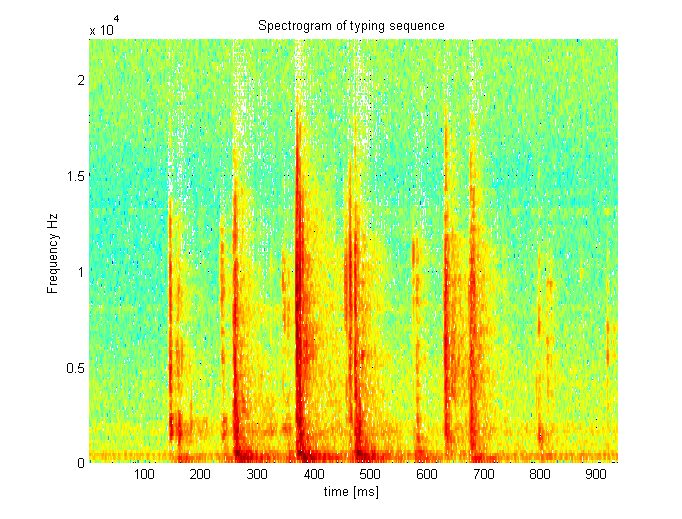
\includegraphics[width=110mm]{shortFastSeqSpec.png}
    \caption{Spectrogram of the same sequence of 5 keystrokes as in Figure~\ref{fig:shortFastSeq.png}. Sampled at 44.1 kHz.}\label{fig:shortFastSeqSpec.png}
  \end{center}
\end{figure}

A thorough investigation of the data associated with this application will be conducted in section~\ref{sec:WPdata}, but with this initial investigation the distinguishing features of interest in keyboard typing pulses are a wide spectral response and rapid onset with lingering low frequency components. The temporal extent of the initial pulses typically range from 30 ms to over 300 ms.

%in the literature (summary)
%A couple of articles have suggested similar systems\cite{Subramanya2007}\cite{Sugiyama2007}\cite{Abramson2007}. \cite{Subramanya2007} and \cite{Sugiyama2007} propose algorithms specifically for the keyboard stroke detection and removal application. All of these methods rely on STFT as a basis for detection using features such as the shape of and change of the power spectrum\cite{Sugiyama2007}, AR estimation error\cite{Subramanya2007}\cite{Kauppinen2002} or a Bayesian speech estimator\cite{Abramson2007}. In \cite{Godsill1998book} various AR based detection methods are proposed and it was found that pairing the AR model with a basis, e.g. a sinusoid, gives a generally applicable approach with improved performance. In \cite{Vaseghi1990} the authors find that AR processes are ``adequate for modelling of speech signals whereas they can not model impulsive disturbances.''.
%
%Restoration approaches applicable to longer gaps ranged from heuristic waveform substitution methods\cite{Goodman1986}\cite{Niediwiecki2001}, pitch based methods modeling speech as spectral peak tracks\cite{Maher1994}\cite{McAulay1986} to AR interpolators\cite{Esquef2006} based on a least squares adaption of the AR process\cite{Godsill1998book}.
%synthesis filters designed to excite the AR model to achieve longer gap extrapolation with lower model orders\cite{Esquef2006}

%\section{Scope of the thesis and contributions to knowledge}

\section{Terminology}
%pulse/impulse
%noise
%Transient noise used when focus on noise.
Throughout the literature the terms \emph{pulse}\cite{Esquef2002a}\cite{Esquef2003a} and \emph{impulse}\cite{Czyzewski1995}\cite{Kauppinen2002a}\cite{Chen2000} have been used interchangeably to refer to a short burst of sound. Generally the use of the term \emph{click}\cite{Czyzewski1995}\cite{Esquef2002}\cite{Godsill1998book} has been associated with physical defects in a recording medium or other extremely short term corruptions. Henceforth the term \emph{pulse} will be used to describe the specific audio signals of interest throughout this work, for its alignment with the already established term acoustic pulse recognition (APR)\cite{TouchSystems2006}. The term \emph{noise}, or the more specific \emph{impulsive noise} and \emph{transient noise}, will only be used to refer to specifically unwanted aspects of the signal and will as such mainly be used in chapters~\ref{ch:TransientNoiseDetection} and \ref{ch:TransientNoiseRestoration}.

%Keyboard stroke pulse (sometimes pulse sequence) vs. single pulse
In chapters~\ref{ch:TransientNoiseDetection} and \ref{ch:TransientNoiseRestoration} the term \emph{keyboard stroke} or \emph{key stroke} will be used to specifically refer to the sequence of disturbances that arise from typing action on a keyboard. These sequences will in many cases encompass a series of \emph{pulses}.

%Chapter~\ref{ch:TransientNoiseRestoration} is commonly referred to as the \emph{restoration} chapter, but the term \emph{reconstruction} has also in some places been applied somewhat interchangeably. In general the term \emph{restore} has been used more generally as any action that aims to alleviate \emph{defects}, \emph{artifacts} or \emph{noise}. \emph{Reconstruct} refers more specifically to situations where samples are discarded and replaced with new estimates. An example of a \emph{restoration} that would not be a \emph{reconstruction} is a scaling action of corrupted samples. In the same chapter the terms \emph{interpolation} and \emph{extrapolation} has been used in some contexts interchangeably. In general \emph{interpolate} is used to refer to action where samples are inserted in between other samples by some means, e.g. linear interpolation, where \emph{extrapolate} refers to the extension of a signal with no pre-defined end points, e.g. prediction. Typically \emph{interpolation} is here more often used to refer to the non-real-time applications that in most cases end up being \emph{extrapolation} when applied in real-time due to the general rule of causality.

\section{Contributions of this thesis}
Work presented in chapter~\ref{ch:APR} is also presented in \cite{Christensen2011} and \cite{US20110316784}.

\section{About this thesis}
This thesis is structured as follows; Following this introductory chapter the literature review is presented in chapter~\ref{ch:LiteratureReview}. Here the surveyed literature is presented in sections relevant to their occurrence in the thesis. Chapter~\ref{ch:APR} introduces the pulse classification or APR system and the main theory. Results are also presented outlining detection performance and the model's sensitivity to certain parameters. Chapter~\ref{ch:MultichannelAPR} presents a multi-channel generalisation of the basic model derived in chapter~\ref{ch:APR}. Results are presented, in Chapter~\ref{ch:MultichannelAPR}, from extensive testing in clean and noisy environments. Chapters~\ref{ch:TransientNoiseDetection} and~\ref{ch:TransientNoiseRestoration} should be considered together as the transient noise suppression system, where chapter~\ref{ch:TransientNoiseDetection} presents methods for the detection of pulses including a proposed pre-processing stage and chapter~\ref{ch:TransientNoiseRestoration} builds on the previous work and considers a number of restoration approaches for the detected pulses. The thesis ends with the conclusions in chapter~\ref{ch:Conclusions}. Here the aims for the work presented in the introduction are reevaluated in the context of the work undertaken. The major contributions are restated and a summary of the proposed future work is presented.

%%% ----------------------------------------------------------------------


%%% Local Variables:
%%% mode: latex
%%% TeX-master: "../thesis"
%%% End:

\chapter{Literature review}\label{ch:LiteratureReview}

\ifpdf
    \graphicspath{{Chapter2_LitReview/Chapter2Figs/PNG/}{Chapter2_LitReview/Chapter2Figs/PDF/}{Chapter2_LitReview/Chapter2Figs/}{Chapter2_LitReview/Chapter2Figs/Classification/}{Chapter2_LitReview/Chapter2Figs/Detection/}{Chapter2_LitReview/Chapter2Figs/Restoration}}
\else
    \graphicspath{{Chapter2_LitReview/Chapter2Figs/EPS/}{Chapter2_LitReview/Chapter2Figs/}}
\fi

The literature review presented in this chapter is split into 3 major sections. Classification, Detection and Restoration. These 3 major areas will generally be dealt with in the order in which they are relevant.

%Not JUST classification. Also some other stuff (needs to be removed)
\section{Classification}\label{sec:LitRev_Classification}
%\subsection{Computational Auditory Scene Analysis (CASA)}
%The CASA approach to source separation attempts to mimic the Auditory Scene Analyzing (ASA) capabilities of the brain by computational means. \cite{Wang2006} state: ``One may define the CASA problem as the challenge of constructing a machine learning system that achieves human performance in ASA''. In an attempt to make CASA systems more \emph{biologically relevant} many CASA systems limit their scope to either monaural or binaural input signals and hence replicating the ASA problem where only the signal from the two ears are present.
%
%More specifically CASA solutions aim to identify certain auditory object, such as characterizing note objects in terms of harmonicity, correlated modulation, duration of sinusoidal partials and common onset, and arranging these into streams using psycho-acoustic cues \citep{Ellis1996}. Proximity of time-frequency objects within the audio mixture can cause problems for CASA whereas ASA is able to retain a reasonable degree of separation of sources. These shortcomings of CASA have thus been the focus of much research. Examples of this is the integration of evidence derived from multiple grouping principles at several levels of abstraction \citep{Godsmark1999}, matching of timbre features learned on solo excerpts \citep{Kashino1998},\citep{Kinoshita1999},\citep{Eggink2003} (based on a Gaussian Mixture Model (GMM) classifier). More recently the overlap probability of frequency components has been introduced to improve algorithm performance \citep{Sakuraba2003}.
%
%CASA methods still suffer from a few drawbacks though. The brain's own ASA system is able to localize sources in a natural acoustic environment through what is known as the \emph{precedence effect}. In environments where a sound is reflected multiple times before reaching the listener, the brain is able to give \emph{precedence} to early arrival of sounds, such as the direct sound, and hence evaluate the true location of the sound. This precedence rule between grouping cues can be hard to assess \citep{Wang2006}, which is also why current methods are restricted to non-reverberant mixtures \citep{Vincent2006}.
%
%In the recent paper, \cite{Shao2010}, the authors present a CASA system for separating speech signals in the presence of other speech or noise. Their approach proceeds by tracking time-frequency units across time frames in 2 different stages. Firstly they use harmonicity to segregate the voiced portions of individual sources for each time frame using multipitch tracking. Secondly the time-frequency units are grouped across the time frames by utilizing knowledge from the speaker characteristics. The system proposed in \cite{Shao2010} mainly focusses on features such as onset/offset and periodicity which are not specific necessarily specific to the target source or even speech and as such this system works well for a variety of speech separation cases with a variety of noise scenarios.
%
%\subsection{Independent Component Analysis (ICA)}
%One of the most widely known and used methods for blind source separation (BSS) is Independent Component Analysis (ICA). ICA proposes to separate a multivariate signals into additive subcomponents supposing the mutual statistical independence of the non-Gaussian source signals. For $M$ observations and $N$ sources it is a requirement for ICA to work that $M\geq N$.
%In general ICA can be defined as the linear transformation $\textrm{\textbf{A}}$ of observed data $\textrm{\textbf{x}} = [x_1,\ldots,x_M]$
%
%\begin{equation}\label{eq:ICA1}
%    \textrm{\textbf{x}} = \textrm{\textbf{A}}\textrm{\textbf{s}}
%\end{equation}
%
%where $\textrm{\textbf{s}}  = [s_1,\ldots,s_N]$ is the separated sources or components \citep{Virtanen2007}.
%
%Traditionally $\textrm{\textbf{A}}$ would then be referred to as the mixing matrix. The source signals $\textrm{\textbf{s}}$ can feasibly be recovered using $\textrm{\textbf{s}} = \textrm{\textbf{A}}^{-1}\textrm{\textbf{x}}$  with $\textrm{\textbf{A}}$ the invertible matrix.  $\textrm{\textbf{A}}^{-1}$ is then called the un-mixing matrix \citep{Smaragdis1998}.
%
%A very popular implementation of the ICA method is the FastICA algorithm as proposed in \cite{Hyvarinen1999}. Often mixture models are modeled as \emph{convolutive} and hence solving for the mixing matrix \textbf{A} in the time-domain will require labor-intensive convolution while some methods propose solutions to the inherent permutation problem for the frequency domain equivalent of the FastICA \citep{Mitianoudis2003}. It has been reported that this approach has also produced good separation results.
%
%A more recent paper \citep{Douglas2007} presents two spatio-temporal extensions to the FastICA method and reports significant improvements over previous methods when applied to multichannel recordings of two- and three-source speech mixtures in a room environment. It was also noted that this proposed method was simple, fast and did not require parameter tuning in order to obtain good separation performance.
%
%\subsubsection{Convolutive mixtures}
%Due to extensive filtering imposed upon real world signals by their environment and propagation delays, instantaneous mixtures are rarely encountered. Most real world mixtures tend to be of convolved mixtures \citep{Smaragdis1998}.
%
%Consider again the model from equation~(\ref{eq:ICA1}) but this time consider a mixture $\textrm{\textbf{x}}$ recorded in a real environment where the mixture can be approximated by a convolutive mixture of the source signals in the time domain,
%
%\begin{equation}\label{eq:ICA2}
%    \textrm{\textbf{x}}(t) = \textrm{\textbf{A}}(t) \ast\textrm{\textbf{s}}(t).
%\end{equation}
%
%Applying the Fourier Transform (FT) yields:
%\begin{equation}\label{eq:ICA3}
%   \hat{ \textrm{\textbf{x}}}(\omega) = \hat{\textrm{\textbf{A}}}(\omega)\hat{\textrm{\textbf{s}}}(\omega),
%\end{equation}
%where $\hat{ \textrm{\textbf{x}}}(\omega), \hat{\textrm{\textbf{A}}}(\omega)$ and $\hat{\textrm{\textbf{s}}}(\omega)$ are the FT of $\textrm{\textbf{x}}(\omega), \textrm{\textbf{A}}(\omega)$ and $\textrm{\textbf{s}}(\omega)$ respectively \citep{Ikeda1999}.
%
%It is noted that if $\textrm{\textbf{A}}$ in equation~(\ref{eq:ICA1}) is seen as a matrix of FIR filters instead of scalars, the resulting multiplication will be equivalent to convolution and the notation will be consistent. This notation is called FIR algebra notation \citep{Lambert1996}.
%
%This time-frequency approach to ICA has been proposed by a variety of authors \citep{Lee1998},\citep{Ikeda1999},\citep{Smaragdis1998} and specifically \cite{Ikeda1999} has been successful in dealing with the inherent arbitrary scaling and permutation problems of the ICA approach applied in a frequency domain context \citep{Zhang2007}.
%
%The recent paper \cite{Zhang2007} attempts to avoid the whitening of outputs which plagues conventional implementations of ICA for convolutive mixtures by enforcing pairwise independence rather than mutual independence. This approach is based on the findings that for blind separation the two are generally equivalent.
%%better ending here?
%
%\subsection{Independent Subspace Analysis (ISA)}
%Independent Subspace Analysis (ISA) is based on ICA but relaxes the constraints $M\geq N$ and the statistical independence of source signals. In practice ISA is a generalization of ICA in the sense that instead of requiring statistical independence between components ISA requires statistical independence between groups of components. ISA can also been described as multidimensional independent component analysis and hence the independent components are required to be of the same dimension $k$. In the case where $k = 1$, ISA is equivalent to ICA \citep{Theis2006}. Despite this relaxing of restrictions of the ICA approach implementations of ISA has still been restricted by fixed group sizes or semi-parametric models. An even more general approach has been proposed which introduces the concept of irreducible independent components and give an identifiability result for this general, parameter-free model together with an arbitrary subspace size algorithm \citep{Theis2006}.
%
%A previous study managed to implement ISA models for audio source separation and introduced the \emph{ixegram} as a measure space for grouping independent basis components \citep{Casey2000}. The separation and grouping results from this experiment suggest that the technique can perform separation of source signals without parametric model fitting or prior knowledge of the composition of input data.
%
%\subsection{Non-Negative Matrix Factorisation (NMF)}
%Since the concept of Non-Negative Matrix Factorization (NMF) was introduced independently by \cite{Paatero1997} and \cite{Lee1999} the method has gained some popularity within the field of polyphonic transcription and the source separation field \citep{Smaragdis2003},\citep{Smaragdis2004}. NMF was originally proposed as an alternative to $k$-means clustering and principal component analysis (PCA) for data analysis and compression.
%The original formulation of NMF starts with a non-negative $M\times N$ matrix $\textrm{\textbf{V}} \in \mathbb{R}^{\geq 0,M\times N}$ where the goal is to approximate $\textrm{\textbf{V}}$ as a product of two non-negative matrices so that
%
%\begin{equation}\label{eq:nmf1}
%    \textrm{\textbf{V}} \approx \textrm{\textbf{W}}\textrm{\textbf{H}}
%\end{equation}
%where $\textrm{\textbf{W}} \in \mathbb{R}^{\geq 0,M\times R}$, $\textrm{\textbf{H}} \in \mathbb{R}^{\geq 0,R\times N}$ and $R \leq M$ such that the error of reconstruction is minimized \citep{Smaragdis2004}.
%
%Good results have generally been reported for extraction of percussive sounds in mono recordings, but for low intensity sounds the algorithms generally perform worse and suffer from distortion and lost information inherent in the mixing and analysis process \citep{Smaragdis2004}. Other results have shown NMF to consistently obtain better separation results than ISA and ICA \citep{Virtanen2007}.
%
%\subsection{Hierarchical Bayesian Models}
%
%The task in Bayesian source separation is to infer $N$ source signals $s_{k,n} \equiv \textrm{\textbf{s}}$ given $M$ observed signals $x_{k,m} \equiv \textrm{\textbf{x}}$, where $n=[1,\ldots,N]$ and $m=[1,\ldots,M]$. Here $k=[1,\ldots,K]$ is an index which may correspond to time or to expansion coefficient of the sources in a linear transform domain. A Hierarchical Bayesian Model for the inference of the source signals can hence be formulated as
%
%\begin{equation}\label{eq:hbm1}
%    p(\textrm{\textbf{s}}|\textrm{\textbf{x}}) = \frac{1}{Z_x}\int p(\textrm{\textbf{x}}|\textrm{\textbf{s}},\Theta_m)p(\textrm{\textbf{s}}|\Theta_p)p(\Theta_p)p(\Theta_m)d\Theta_m d\Theta_p.
%\end{equation}
%
%Here the conditional distribution is characterized by the conditional distribution $p(\textrm{\textbf{x}}|\textrm{\textbf{s}},\Theta_m)$, where $\Theta_m$ denotes the collection of mixing parameters such as the mixing matrix, observation noise and variance, etc. and the prior term $p(\textrm{\textbf{s}}|\Theta_p)$ describes the sources via their own prior parameters $\Theta_p$ \citep{Cemgil2007}.
%
%It is worth noting that there is a considerable computational cost associated with a full Bayesian inference, via MCMC or Variational Bayes for Bayesian source separation (VB). Good results were reported in a study attempting Bayesian source separation using an MCMC approach to inference \citep{Fevotte2006}. Also, the authors of this study point out the computational burden of the MCMC approach compared to the alternative Expectation Maximisation (EM) approach. It was although also noticed that the EM approach was far more sensitive to mixing matrix initialization and hence less robust. The Gibbs sampler described in this paper was implemented as part of the review of this paper. Although the implementation was problematic due to the inherent indeterminacy on gain, the approach provided good results to noisy linear mixtures of sources.
%
%The recent paper \cite{Cemgil2007} describes a hybrid approach where a general linear instantaneous model, which might be noisy and underdetermined, is tackled using a Student $t$ distribution to model the source prior. Both the Gibbs sampler and VB method were studied as a method for inference. Both these methods are algorithmically similar but by employing a hybrid method the authors managed to combine the speed of the variational approach with the robustness of the Gibbs sampler \citep{Cemgil2007}.

\subsection{TBC}
\todo{general classification lit rev}


\subsection{Principal Component Analysis (PCA)}
The central idea of PCA is to reduce the number of dimensions of a set of data consisting of possibly correlated variables to a smaller number of uncorrelated variables. This operation is achieved by transforming to a set of uncorrelated variables, principal components (PCs), which are ordered so the first PC retain most of the variability and each succeeding component accounts for as much of the remaining variability as possible.

Take $\textrm{\textbf{x}}$ to be a vector of $p$ random variables where the variance of the variables and the correlation or covariance between them are of interest. The approach taken by PCA is to look for a few ($<<p$) derived variables which preserves most of the information given by these variances and covariances or correlations. The initial step is to look for a linear function $\boldsymbol\alpha_1^T \textrm{\textbf{x}}$ of $\textrm{\textbf{x}}$ which maximizes the variance, where $\boldsymbol\alpha_1^T =  [\alpha_{1{}1},\alpha_{1{}2},\ldots,\alpha_{1{}p}]$ so that:

\begin{equation}\label{eq:PCAdef}
\boldsymbol\alpha_1^T \textrm{\textbf{x}}= \alpha_{1{}1}x_1 +\alpha_{1{}1} x_2 + \ldots \alpha_{1{}p} x_p = \sum^p_{j=1}\alpha_{1{}j}x_j,
\end{equation}

is the first PC where ${}^T$ denotes a transposed matrix.
Now, find the linear function $\boldsymbol\alpha_2^T \textrm{\textbf{x}}$ of $\textrm{\textbf{x}}$ uncorrelated with $\boldsymbol\alpha_1^T \textrm{\textbf{x}}$ which again maximizes the variance, and so on, so that the $k$th PC $\boldsymbol\alpha_k^T \textrm{\textbf{x}}$ maximizes the variances while being uncorrelated to $\boldsymbol\alpha_1^T \textrm{\textbf{x}}, \boldsymbol\alpha_2^T \textrm{\textbf{x}}, \ldots, \boldsymbol\alpha_{k-1}^T \textrm{\textbf{x}}$. For a reduction of dimensionality it is hoped that most of the variability of $\textrm{\textbf{x}}$ is accounted for by $q$ PCs where $q<<p$ \citep[chap. 1]{Jolliffe1986}.

A more common transform into uncorrelated basis functions is the Discrete Fourier Transform (DFT) or FT which decomposes a signal into a set of uncorrelated or orthogonal (in the statistical sense) complex exponentials of the form $e^{i\omega t}$. The transform described above can therefore be seen as a generalization of the DFT for random processes, where the decomposed uncorrelated basis functions are real random signals rather than complex exponentials \citep[chap. 4.6]{Therrien1992}.

\subsection{Simple PCA Examples}

Figure~\ref{fig:30observations} gives a plot of 30 observations of two highly correlated (non zero mean) variables $x_1$ and $x_2$. It is seen that although there are considerable variation in the two variables, it is also noticed that there is more variation in the direction $x_2$.
\begin{figure}[!]
  \begin{center}
    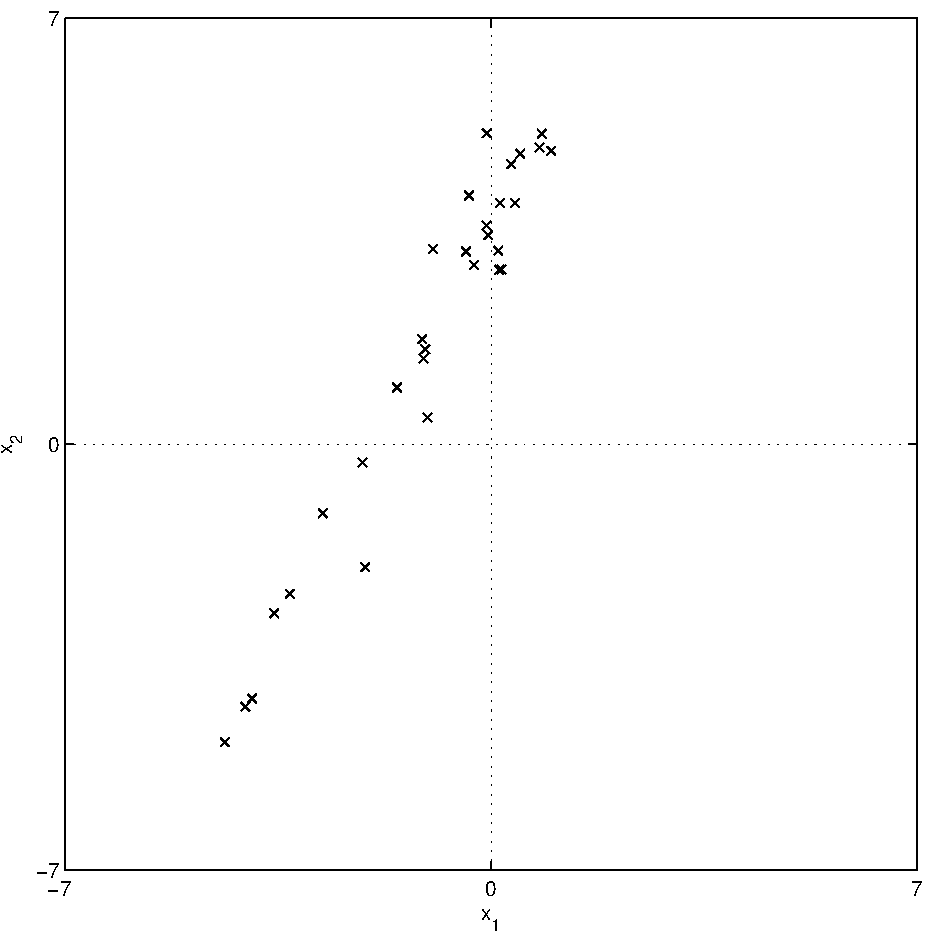
\includegraphics[width=260px]{30observations.pdf}
    \caption{Plot of 30 observations of variables $x_1$ and $x_2$.}\label{fig:30observations}
  \end{center}
\end{figure}

It is also seen in Figure~\ref{fig:30observations} that neither of the two variables are zero mean. To apply PCA the mean of both variables must be subtracted. Figure~\ref{fig:30observationsBar} shows the two variables with their means subtracted.
\begin{figure}[!]
  \begin{center}
    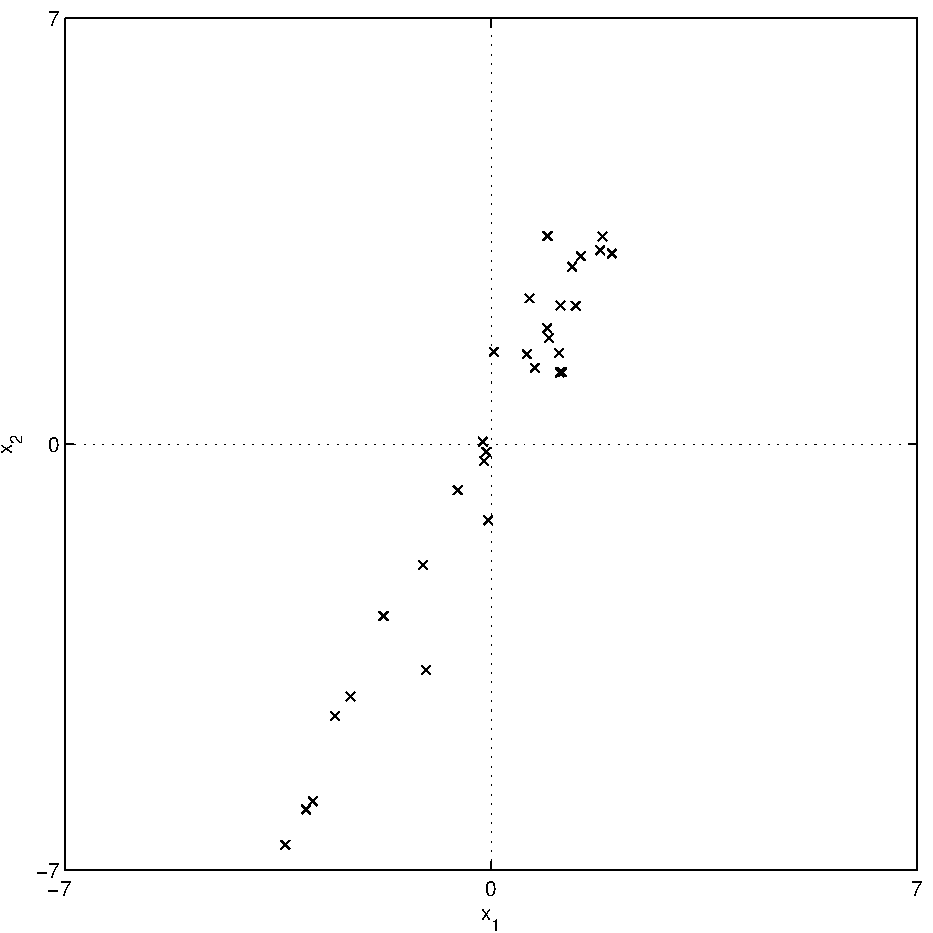
\includegraphics[width=260px]{30observationsBar.pdf}
    \caption{Plot of 30 observations of variables $x_1$ and $x_2$ with means subtracted.}\label{fig:30observationsBar}
  \end{center}
\end{figure}

Since the process of PCA is closely related to the diagonalization of the correlation matrix \citep[p. 174]{Therrien1992}, a helpful interpretation of the PCA is the attempt to ``rotate'' the axes of Figure~\ref{fig:30observationsBar} to collect as much variability as possible in one dimension, rather than having it spread over 2 dimensions. The correlation matrix (correlation coefficients) for the two variables $x_1$ and $x_2$ is,

\begin{equation}\label{eq:corrcoef}
\textrm{Correlation matrix} = \textrm{corr}(x,y)= \left(
    \begin{array}{cc}
        1   & 0.97 \\
        0.97& 1    \\
    \end{array}\right),
\end{equation}
where the correlated nature of the two variables is clearly seen by the almost unitary off-diagonal terms. Since the covariance matrix $\boldsymbol\Sigma$ is square it is possible to look at the eigenvalues and eigenvectors of it, which are,

\begin{eqnarray}\label{eq:eigValues}
\textrm{Eigenvalues} &=& \boldsymbol\lambda = \left(
    \begin{array}{c}
        \lambda_1 \\
        \lambda_2 \\
    \end{array}\right) = \left(
    \begin{array}{c}
        11.85 \\
        0.107 \\
    \end{array}\right)\\\label{eq:eigenVectors}
    \textrm{Eigenvectors} &=& \boldsymbol\alpha = \left( \boldsymbol\alpha_1 \quad \boldsymbol\alpha_2\right) =\left(
    \begin{array}{cc}
         0.451 & -0.892  \\
         0.892 & 0.451   \\
    \end{array}\right).
\end{eqnarray}

The eigenvectors from equation~(\ref{eq:eigenVectors}) have been plotted on top of the data in Figure~\ref{fig:30observationsBarEig}. These eigenvectors reveal information about patterns in the data, and as expected a clear correlation is found by the eigenvector $\boldsymbol\alpha_1$ between the variables $x_1$ and $x_2$. The second eigenvector $\boldsymbol\alpha_2$ gives the other, less important, pattern in the data.

\begin{figure}[!]
  \begin{center}
    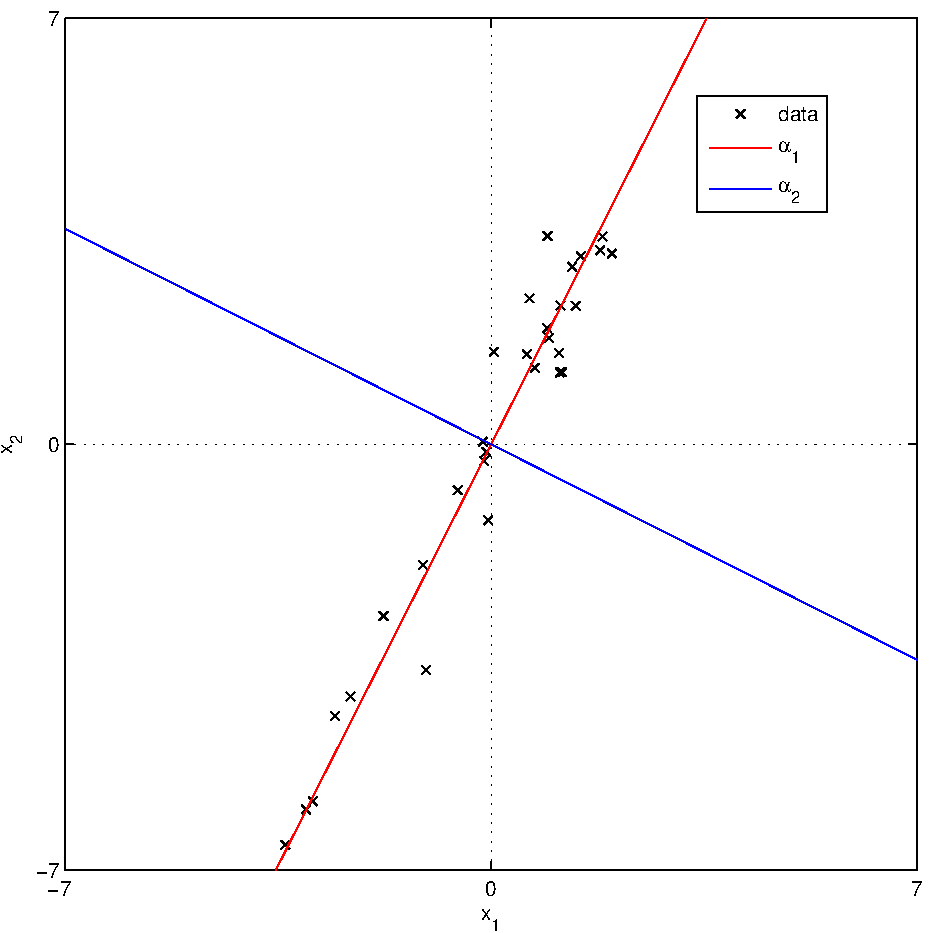
\includegraphics[width=260px]{30observationsBarEig.pdf}
    \caption{Plot of 30 observations of variables $x_1$ and $x_2$ with means subtracted, and eigenvectors of covariance matrix $\boldsymbol\Sigma$ plotted on top of the data. $\boldsymbol\alpha_k$ refers to the $k$th eigenvector.}\label{fig:30observationsBarEig}
  \end{center}
\end{figure}

The eigenvector with the highest corresponding eigenvalue is the PC. Ordering the eigenvectors in terms of descending eigenvalue gives the components in order of significance. It turns out that, for $k \in \{1, 2, \ldots, p\}$ the $k$th PC is given by $z_k = \boldsymbol\alpha_k^T\textrm{\textbf{x}}$, where $\textrm{\textbf{x}} = [x_1,x_2,\ldots, x_p]^T$ and where $\boldsymbol\alpha_k$ corresponds to the eigenvector with the $k$th largest eigenvalue \citep[p. 2-3]{Jolliffe1986}. For a complete transformation of the data use the expression $\textrm{\textbf{z}} = \hat{\boldsymbol\alpha}^T\textrm{\textbf{x}}$ where $\hat{\boldsymbol\alpha}$ is the feature vector containing the number of eigenvectors desired $q$, so $\hat{\boldsymbol\alpha} = [\boldsymbol\alpha_1,\boldsymbol\alpha_2,\ldots,\boldsymbol\alpha_q]$. Figure~\ref{fig:30observationsBarEig} shows the transformed data in terms of the transformed variables $z_1$ and $z_2$.

\begin{figure}[!]
  \begin{center}
    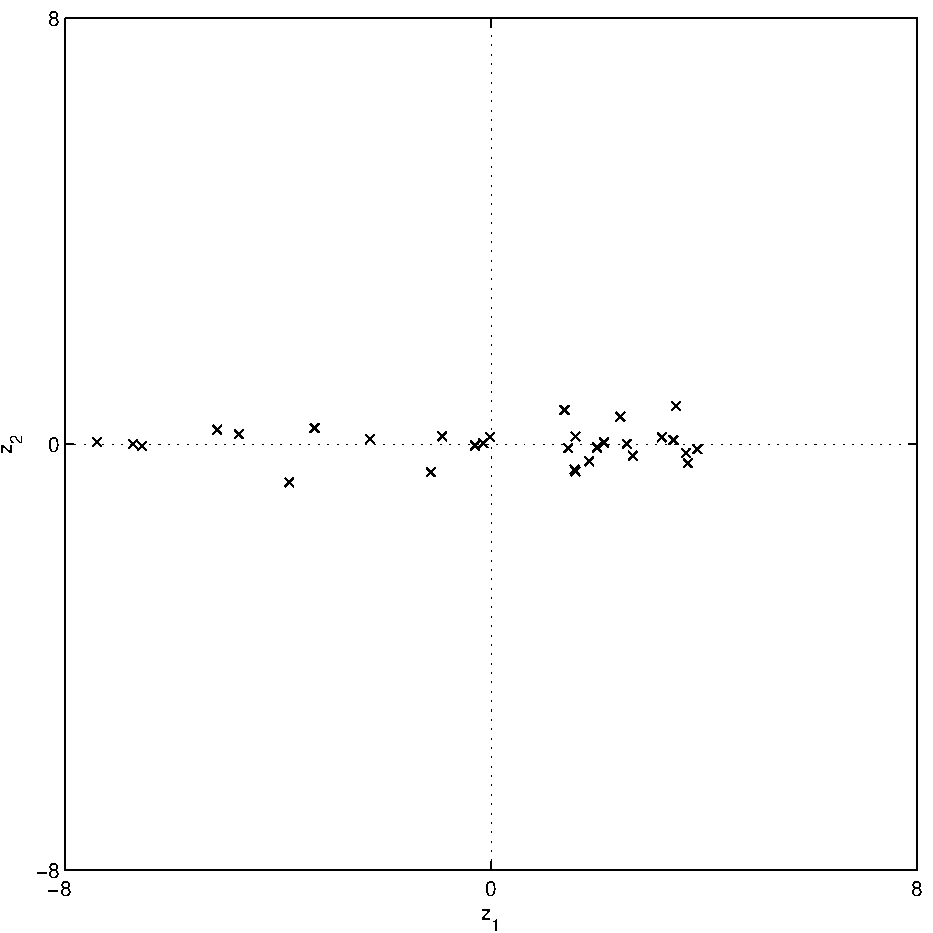
\includegraphics[width=260px]{30observationsBarTrans.pdf}
    \caption{Plot of 30 observations of variables $x_1$ and $x_2$ transformed into $z_1$ and $z_2$. Almost all the information or variability is now in $z_1$.}\label{fig:30observationsBarTrans}
  \end{center}
\end{figure}

It is noticed that this transform, who's results are displayed in Figure~\ref{fig:30observationsBarEig}, do not actually reduce the dimensionality of the data since $q=p$ and hence all information is preserved. By making $q<p$ the dimensionality is reduced and less significant data is discarded. Since it is noticed from equation~(\ref{eq:eigValues}) that $\lambda_1$ is much larger than $\lambda_2$, and hence $\boldsymbol\alpha_1$ is a far more significant component in the data than $\boldsymbol\alpha_2$, one could feasibly define the feature vector as $\hat{\boldsymbol\alpha} = \boldsymbol\alpha_1$. Figure~\ref{fig:30observationsFinal} shows the result of a transformation of the 30 observations for this scenario where $q=1$. The data has been transformed back into $x_1$ and $x_2$ and the original means of the data has been reapplied.

\begin{figure}[!]
  \begin{center}
    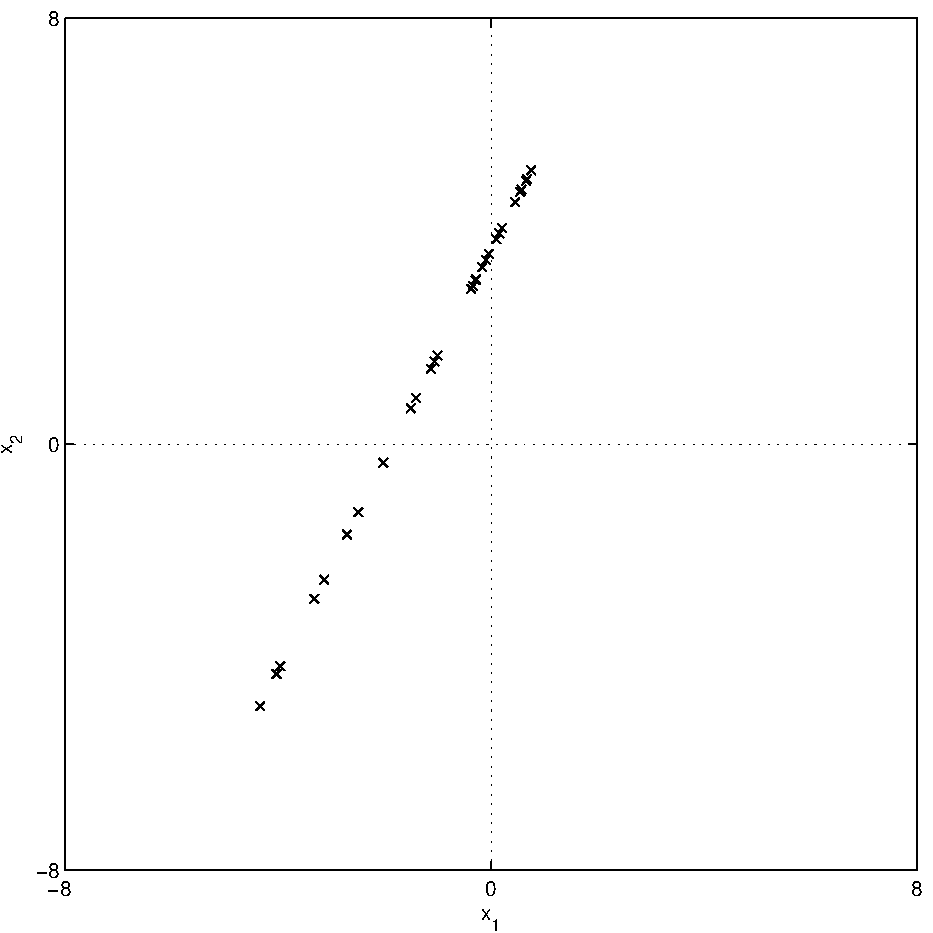
\includegraphics[width=270px]{30observationsFinal.pdf}
    \caption{Plot of 30 observations of variables $x_1$ and $x_2$ transformed from only $z_1$ with original means added back in.}\label{fig:30observationsFinal}
  \end{center}
\end{figure}

It is clearly seen how the data resembles that of Figure~\ref{fig:30observations} although some of the variability has been lost in the dimensional reduction.

\subsubsection{Eigenfaces}
A popular application of PCA is the so called \emph{eigenfaces}. \emph{Eigenfaces} are essentially eigenvectors derived from the covariance matrix of a high dimensional vector space or ensemble of individual pictures. The idea of \emph{eigenpictures} was originally developed by \cite{Sirovich1987} were the authors repeatedly draw parallels between how humans recognize facial features and their own computational method. Although the \emph{eigenpictures} were not formerly used for facial recognition until \cite{Turk1991}, where the term \emph{eigenfaces} was first coined, \cite{Sirovich1987} hypothesises that perhaps humans compartmentalize faces and treat different features individually. This assertion is rooted first in the observation that humans are able to store and recognize enormous numbers of faces and secondly, that since recognition is apparently instantaneous it is conceivable that we do it by some efficient method, possibly similar to low dimensional methods. It is for example noted that ``(...) fewer than 100 \emph{eigenpictures} are necessary to fit a picture.'' and ``fewer than 100 dimensions are needed to provide likeness.''.

The method used in \cite{Sirovich1987} uses photographs of 115 male undergraduates faces. These pictures were then digitized to a 128 by 128 pixel image and manually aligned. Figure~\ref{fig:Sirovich1987-3} shows a figure of 3 cropped images. The left image is the average face based on the ensemble, the middle is a sample face and right image that sample faces departure from the ensemble average or the samples \emph{caricature}. All pictures presented in this section are reproduced from the original paper \cite{Sirovich1987} where none of the pictures have been filtered to eliminate the high frequencies produced by digitization.

\begin{figure}[!]
  \begin{center}
    \includegraphics[width=410px]{Sirovich1987-3.pdf}
    \caption{Cropped faces: left, the average; middle, a sample face; right, its caricature.}\label{fig:Sirovich1987-3}
  \end{center}
\end{figure}

The covariance matrix of the aligned ensemble is now calculated and all the \emph{eigenpictures} determined. Figure~\ref{fig:Sirovich1987-4} shows the first 8 of these \emph{eigenpictures} going from the top left frame, moving right and ending on the bottom right frame with the 8th \emph{eigenpicture}.

\begin{figure}[!]
  \begin{center}
    \includegraphics[width=270px]{Sirovich1987-4.pdf}
    \caption{First 8 \emph{eigenpictures} starting at upper left, moving to the right, and ending at lower right.}\label{fig:Sirovich1987-4}
  \end{center}
\end{figure}

Figure~\ref{fig:Sirovich1987-5} shows the approximate reproduction of the sample face from Figure~\ref{fig:Sirovich1987-3} reproduced using 10, 20, 30 and 40 components.

\begin{figure}[!]
  \begin{center}
    \includegraphics[width=270px]{Sirovich1987-5.pdf}
    \caption{Approximation of the original picture (middle picture of Figure~\ref{fig:Sirovich1987-3}) using 10, 20, 30 and 40 \emph{eigenpictures}.}\label{fig:Sirovich1987-5}
  \end{center}
\end{figure}



\subsubsection{In the literature}
As mentioned previously, one of the main applications of PCA is dimensionality reduction which has rendered it useful in a variety of compression applications. Within the image compression community \citep{Vasilescu2003} the focus on PCs has been useful in dimensionality reduction, and more specifically it has been widely applied as a way of representing animations of 3D geometric shapes. \cite{Alexa2000} presented an ``easy and adaptive lossy compression'' algorithm which provided compression of animation sequences with a factor of 1:100 accepting loss in animation accuracy. Another approach to animation compression is presented in \cite{Karni2004} where PCA is combined with Linear Prediction Coding (LPC) to individually focus on spatial and the resulting temporal components respectively.

Although PCA is optimal in approximating the input data in the mean-squared error sense, the representation that it provides is often not the most meaningful in terms of real world data and in terms of describing the fundamental properties of the data. Since the PCA describes the data in an orthonormal basis, purely in order of the second-order statistics (covariance) of the input data \citep{Oja1995}, which in effect means that PCA is networks are only able to realize linear input-output mappings \citep{Karhunen1995}. In the field of neural networks there has been an interest in the development of nonlinear PCA methods that take higher-order statistics into account.

Although not specifically a PCA approach, \cite{Honkela2005} presents an approach to general nonlinear generative model for non-linear factor analysis which can form the basis for many non-linear implementations of latent variable models such as a non-linear generalization of PCA or even ICA. This general model is based on the variational Bayesian framework, which forms a solid foundation for non-linear modeling \citep{Honkela2005}. This model can be implemented into a linear ICA framework for nonlinear BSS, and especially \cite{Valpola2003} found that the variational Bayesian method provided ``useful'' results for difficult nonlinear problems. \citep{Lappalainen2000} introduced nonlinear counterparts of PCA and ICA where the generative mapping from sources to data is not restricted to being linear. Here this mapping is modeled by a multi-layer perceptron (MLP) network and the distributions of source signals are modeled by Gaussians. The general form of the models discussed in this paper are of the form:

\begin{equation}\label{eq:nonlinear}
\textbf{x}(t) = f\left(\textbf{s}(t)\right) + \textbf{n}\left(t\right),
\end{equation}

where $\textbf{x}(t)$ are the observations at time $t$, $\text{s}(t)$ are the sources, $\textbf{n}(t)$ the noise and $f()$ the function which maps the sources to the observation space. In \cite{Lappalainen2000} the authors compare their approach favorably to previously suggested models for representing data with nonlinear coordinate systems, and they especially focus on their methods applicability in high dimensional applications.

%*** Check for more recent papers by MacKay ***

\todo{ADD new stuff}
\cite{Burke2013}

\subsection{Probabilistic PCA (PPCA)}
One of the notable features of the above derived definition of the PCA is the lack of a probabilistic model for the observed data. \cite{Tipping1999} proposes a latent variable model for determining the principal axis of observed data which is closely related to factor analysis. This model utilizes a Maximum Likelihood (ML) estimator to estimate the parameters of the latent variable model. This model is commonly known as a factor analysis model where the relationship is linear:

\begin{equation}\label{eq:facAn}
\textrm{\textbf{t}} = \textrm{\textbf{W}}\textrm{\textbf{x}} + \boldsymbol\mu + \boldsymbol\epsilon,
\end{equation}

in which the $d$-dimensional observations vector \textbf{t} is related to a corresponding $q$-dimensional vector of latent (or unobserved) variables \textbf{x}. The $d \times q$ matrix \textbf{W} relates the two sets of variables, $\boldsymbol\epsilon$ is a zero-mean Gaussian noise process and the parameter $\boldsymbol\mu$ allows for model to have a non-zero mean. By defining $\textrm{\textbf{x}} \sim \mathcal{N}_\textrm{x}(\boldsymbol0,\textrm{\textbf{I}})$ and $\boldsymbol\epsilon \stackrel{i.i.d.}{\sim} \mathcal{N}_\epsilon(\boldsymbol0,\boldsymbol\Psi)$, equation~(\ref{eq:facAn}) induces a Gaussian distribution for the observations $\textrm{\textbf{t}} \sim \mathcal{N}(\boldsymbol\mu,\textrm{\textbf{W}}\textrm{\textbf{W}}^T + \boldsymbol\Psi)$. The parameters of this model can then be obtained through an iterative process using ML \citep{Tipping1999}.

\cite{Lawrence2005} presents an extended PPCA model based on the work of \cite{Tipping1999} termed Dual Probabilistic PCA (DPPCA). The DPPCA method can, through Gaussian processes, non-linearize the linear mappings from the embedded space and hence provide new probabilistic approach to visualizing and modeling of high dimensional data.

\section{Detection}\label{sec:LitRev_Detection}
Any restoration of transient noise events presupposes complete knowledge of the position of the corruption. In practice this information is unknown \emph{a priori} and a detection procedure must be employed to ascertain the timing of the corruptions. As noted in this section, a large number of different approaches to transient noise detection has been studied, and since there are as many types of transient noise as there are data that can be corrupted by it, the detection methods range from simple \emph{ad hoc} filtering approaches to more complicated model based approaches.

In a reconstruction algorithm it is important to focus our attention on audible corruptions. The audibility of a corruption is not only a function of its amplitude or the energy that it represents, but also the context in which is sits. Psychoacoustically some corruptions may be rendered inaudible through masking effects such as the precedence effect, and hence any restoration effort is wasted or potentially damaging.\todo{Add citation for (An Introduction to the Psychology of Hearing)}

The simplest pulse detection algorithms exploit the relatively sparse nature of many audio, and in particular speech, signals above 9000 Hz in relation to impulsive noise which often exhibits a much smoother and wider frequency characteristics \cite{Subramanya2007}. In \cite{Kasparis1993}\cite{US6795559} the authors preprocess their signals using a High Pass filter to target to the impulsive noise.

\subsection{Median filter methods}\label{sec:LitRevDetMedianFilts}
A classic pulse noise detection (and restoration) scheme has involved a median filter\cite{Tukey1974}\cite{Lee1985}\cite{Heinonen1985}\cite{Heinonen1987}\cite{Maekivirta1991}\cite{Kasparis1993}.
%explain median filtering
Median filtering for signal smoothing, first published in \cite{Tukey1974}, has, according to \cite{Brillinger2002}, some important characteristics in that they reduce ``spiky'' noise while preserving jump discontinuities (edges). In \cite{Lee1985} it is noted that the media filter has limited effect on non-impulsive noise and the authors propose a method for augmenting the median filter with a linear filter for added smoothing. This augmentation of the nonlinear media filter approach with a linear filtering approach has become a popular variation of median filtering process for impulsive noise detection and reduction spawning a variety of implementations \cite{Lee1985}\cite{Heinonen1985}\cite{Nieminen1987}\cite{Kasparis1993}\cite{Loveridge1995}. In \cite{Kauppinen2002} it was also noted that the pulse detection algorithm that performed best was the median filter preprocessed by a linear filter. In recent years median based algorithms such as weighted median (WM) filters \cite{Yin1996}\cite{Wang2010} and switching median filters \cite{Abreu1996}\cite{Chen2000}\cite{Chen2001}\cite{Lin2007} have seen a fair bit of attention although the focus of the implementations have almost exclusively been focused on image data.

The authors of \cite{Chandra1998} employ the SD-ROM (Signal Dependent Rank Order Mean) algorithm, similar to the media filter methods, to evaluate the likelihood of each sample being corrupted based on the neighbouring samples. While this algorithm has shown great results in the removal of pulse noise in images \cite{Abreu1996} in \cite{Chandra1998} the method performs best for short, although frequent, noise pulses of the order of a single or a few samples.

Since transient noise events often exhibit a sudden fast change in the signal, one way to detect the onset of a noise event is to detect abrupt nonstationary changes in the dynamics of time series. In \cite{Fancourt2000} the authors employ neural network predictors for this task, while \cite{Kauppinen2002} proposes an iterative discrete derivative method. In \cite{Kauppinen2002} the linear predictor and median hybrid method outperformed the derivative approach and the method described in \cite{Fancourt2000} was never tested on real data but the requirement for training and the inherent detection deadzone does reduce the method's general applicability.

\subsection{Autoregressive (AR) methods}\label{sec:LitRevAR}
While autoregressive (AR) methods have been used in other fields for detection and restoration of transient noise events \cite{Arakawa1986} these methods were generally pioneered in the field of audio processing in \cite{Vaseghi1988thesis}\cite{Vaseghi1988}\cite{Vaseghi1990}. AR methods are today the basis for many pulse detection algorithms in audio applications\cite{Karjalainen1997}\cite{Esquef2000}\cite{Haermae2000}\cite{Esquef2002}\cite{Kauppinen2002}\cite{Wolfe2005}\cite{Subramanya2007}. The AR method proceeds by considering a sub-frame of the audio data $x_t$ for $ t = \{ 1, \ldots, N \}$. Assuming the data is drawn from a short-term stationary AR process:

\begin{equation}\label{eq:ARmodel}
x_t = \sum_{i=1}^P a_i x_{n-i} + e_t,
\end{equation}

where $e_t$ is the prediction error (or excitation signal) and $\mathbf{a} = \{a_1,\ldots,a_P\}$ is the AR coefficients of order $P$. The transient nature of the impulsive noise pulses will most likely lead to very large prediction errors if an attempt is made to predict its values with previous values of $x_t$. It follows that if an inverse AR filter is applied to an AR signal segment corrupted with transient noise events $y_t$, the prediction error $e_t = y_t - \sum_{i=1}^P a_i y_{n-i}$ is expected to be large when noise events are present while remaining low at other times\cite{Godsill1998book}.

In \cite{Vaseghi1990} the authors find that linear prediction systems, or AR process, are ``adequate for modelling of speech signals whereas they can not model impulsive disturbances.''. This realisation is used to separate out the residual of the LPC model effectively leaving the excitation noise in addition to the transient noise events, similarly to the pre-processing step of the favored approach in \cite{Kauppinen2002}.

A noisy speech signal $y_n$ can be modelled as an instantaneous mixture of a speech signal $x_n$ and some some impulsive disturbance:

\begin{equation}\label{eq:Vaseghi1990_1}
y_n = x_n + d_n,
\end{equation}

and assuming that the speech signal can be modelled with a linear prediction model,
\begin{equation}\label{eq:Vaseghi1990_4}
x_n = \sum^P_{k=1} a_k x_{n-k} +ge_n,
\end{equation}
where $\mathbf{a}$ is the LPC parameters, $e_n$ is the excitation signal and $g$ is the linear prediction system's gain. The excitation signal can either be noise-like or a mixture of noise and some quasi periodic train of pulses. White noise is considered a good excitation signal for speech modelling\cite{Vaseghi1990}.

Equation~\ref{eq:Vaseghi1990_1} can now be rewritten
\begin{equation}\label{eq:Vaseghi1990_5}
y_n = \sum^P_{k=1} a_k x_{n-k} + e_n + d_n.
\end{equation}

With an estimate for the LPC parameters $\mathbf{\hat{a}}$, the noisy signal $y_n$ can be written as the noisy excitation signal $v_n$

\begin{eqnarray}
% \nonumber to remove numbering (before each equation)
  v_n &=& y_n - \sum^P_{k=1} \hat{a}_k y_{n-k} \nonumber\\
  &=& x_n + d_h - \sum^P_{k=1} (a_k - \tilde{a}_k)(x_{n-k} + d_{n-k}),\label{eq:Vaseghi1990_6}
\end{eqnarray}

where $a_k$ is the error in the LPC parameter vector estimate. Equation~\ref{eq:Vaseghi1990_6} can now be rewritten

\begin{equation}\label{eq:Vaseghi1990_7}
v_n = e_n + d_h - \sum^P+{k=1} \hat{a}_k d_{n-k} + \sum^P_{k=1} \tilde{a}_k x_{n-k}.
\end{equation}

The three elements that contribute to the noise in the excitation sequence estimate is therefore the impulsive disturbance $d_n$, the past noise samples $p$ and the inflation in the variance of the the residual signal due to the error parameter estimate\cite{Vaseghi1990}.

\todo{maybe more sources for the separation?}

Since the transient noise pulses are transformed to a scaled version of the pulse response of the inverse LPC filter, and since experimental results conducted by \cite{Vaseghi1990} shows the amplitude of the excitation signal is in the order of $10^{-1}$ to $10^{-4}$ the detection task is greatly simplified. The authors of \cite{Godsill1998} note that the disadvantages with the approach outlined in \cite{Vaseghi1990} is the inability to detect small pulses in the presence of much larger disturbances as well as the introduction of distortion for certain signals. In \cite{Godsill1998} the pulse detection problem is put in a Bayesian framework and extended to non-Gaussian noise pulses.

An adaptation to the basic AR detection method in \cite{Vaseghi1988} uses a matched filter approach to detect transient noise events. The matched filter approach proceeds by considering the transient noise event as the signal and the AR data as the coloured additive noise. \todo{more on matched filter approach. Possibly also some theory}
An inherent problem with the matched filter is its dependence on training. Other methods in the literature model impulsive noise as non-Gaussian heavy-tailed distributions whereof the $\alpha$-stable distribution is particularly popular \cite{Tsihrintzis1997}\cite{Coates2002}. According to \cite{Nikias1995} $\alpha$-stable distributions are good for modeling many types of impulsive noise (including atmospheric and underwater acoustic noise). While the sub-Gaussians methods in \cite{Tsihrintzis1997}\cite{Coates2002} appear to perform well on certain kinds of impulsive noise it is questionable whether they could perform in a real time application with high pulse variability and high sample rates.

Figure~\ref{fig:LitRev_DetectCompare} and~\ref{fig:LitRev_DetectCompare2} compares the output of 4 basic detections schemes discussed up until now. The data presented in Figure~\ref{fig:LitRev_DetectCompare}(a) and Figure~\ref{fig:LitRev_DetectCompare2}(a) is speech data corrupted with keyboard tapping noise sampled at 44.1 kHz. Each primary tapping pulse has been marked as ``Ground Truth'' although secondary pulses can also be seen. Comparing the matched filter (b) and AR prediction error (c) methods in Figures~\ref{fig:LitRev_DetectCompare} and~\ref{fig:LitRev_DetectCompare2} is is noted that the matched filter produces a more smeared response while, in some cases, picking out more subtle pulses\cite{Godsill1998book}, e.g. 3rd marked pulse in Figure~\ref{fig:LitRev_DetectCompare}.
\todo{Compare (d) and (e) in figures... but mention that they are similarly performing for this data.}

\begin{figure}[!] %LitRev_DetectCompare
\centering
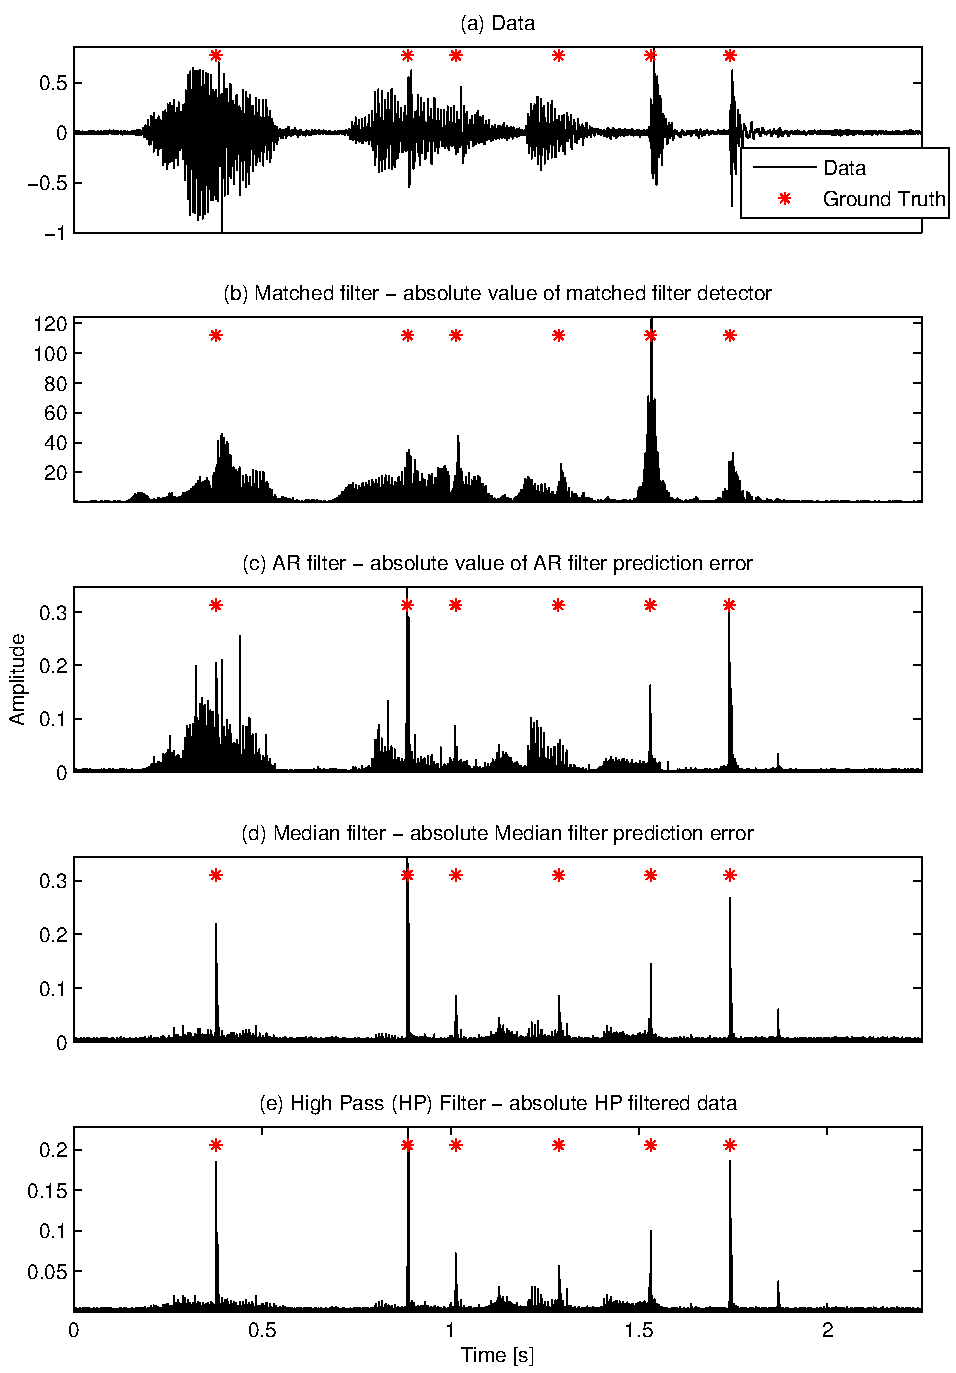
\includegraphics[width=130mm]{LitRev_DetectCompare.pdf}
\caption{Pulse detection comparison, (a) Speech data with 6 primary keystroke pulses sampled at 44.1 kHz, (b) absolute value matched filter detector output, (c) absolute value of AR filter prediction error output, (d) absolute value of median filter prediction error, and (e) absolute value of high pass filtered data with crossover frequency 9.6 kHz.}
\label{fig:LitRev_DetectCompare}
\end{figure}

\begin{figure}[!] %LitRev_DetectCompare2
\centering
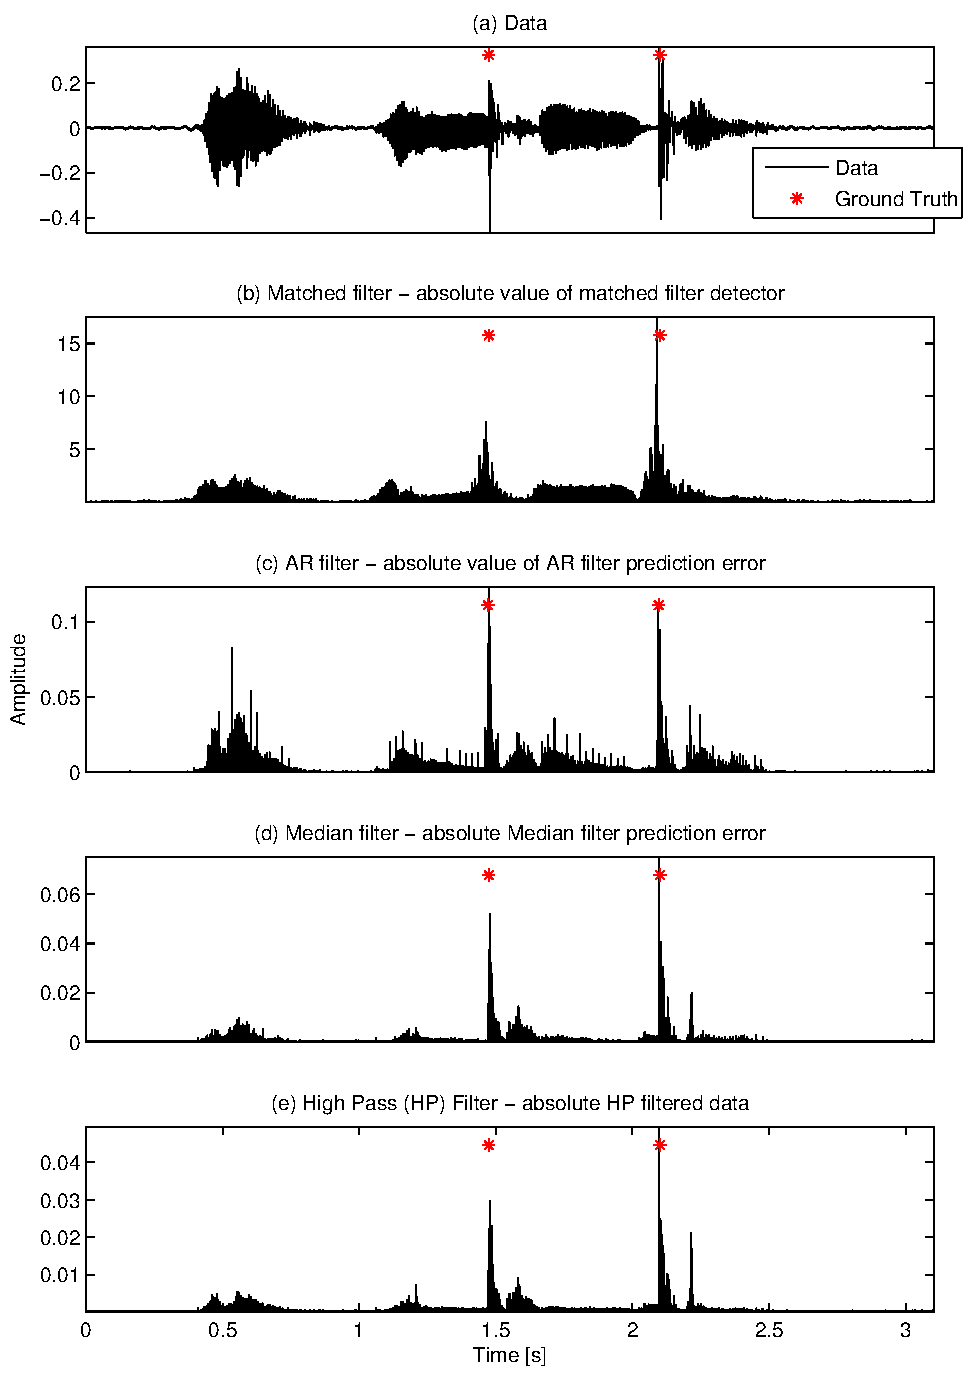
\includegraphics[width=130mm]{LitRev_DetectCompare2.pdf}
\caption{Pulse detection comparison, (a) Speech data with 2 primary keystroke pulses sampled at 44.1 kHz, (b) absolute value matched filter detector output, (c) absolute value of AR filter prediction error output, (d) absolute value of median filter prediction error, and (e) absolute value of high pass filtered data with crossover frequency 9.6 kHz.}
\label{fig:LitRev_DetectCompare2}
\end{figure}

%Warped linear prediction
Warped Linear Prediction (WLP) is another adaptation of the AR method \cite{Esquef2002}. The basic area of \emph{warped} DSP was first introduced in \cite{Oppenheim1983} and later formalized in a predictive framework in \cite{Strube1980} and as a recursive filter\cite{Steiglitz1980}. WLP has since been applied successfully to several audio applications \cite{Karjalainen1997}\cite{Haermae2000} and more specifically used as a basis for pulse detection \cite{Esquef2000}\cite{Esquef2002}.

The basic concept of warped filters can be explained by considering a standard FIR-like structure, but rather than applying the standard unit delay $z^{-1}$ the warped filter applies a new delay element $D(z)$ so that each new delay is frequency dependant (dispersive). In practice this means that the design of the warped filters are based on any pair of functions, $\tilde{z} = f(z)$ and $z = g(\tilde{z})$, so that $f(\cdot)$ and $g(\cdot)$ are one-to-one mappings of the unit circle onto itself, and $z = g\left( f(z) \right)$\cite{Karjalainen1997}. Bilinear conformal mapping\cite{Brown1996} conforms to the requirements and corresponds to the first order allpass filter

\begin{equation}\label{eq:Karjalainen1997}
\tilde{z}^{-1} = D(z) = \frac{z^{-1} - \lambda}{1 - \lambda z^{-1}},
\end{equation}

where $\lambda, -1 < \lambda < 1$, is a warping parameter which, if chosen appropriately \cite{Karjalainen1997}, yields a good match to the psychoacoustic Bark scale\cite{Smith1995}.

Warped digital filters have a range of advantages in that they can be designed to model the human auditory system as well as other physical systems\cite{Karjalainen1997}. In \cite{Esquef2002} the authors note that for auditory models the warping factor $\lambda$ tend to be positive while for click detection negative warping factors appeared to perform best. It was also noted that pulse detection using WLP came at a computational cost and was therefore not suited for real time implementations. As in \cite{Godsill1998book} the authors of \cite{Esquef2002} only considered pulses with duration of $<1 ms$, for which the WLP based method performs well. This is largely believed to be caused by spectral characteristics also exploited in \cite{Kasparis1993}\cite{US6795559}, although the signals in \cite{Esquef2002} were not exclusively corrupted speech data and can therefore not be assumed to be spectrally sparse at high frequencies.


%|P. A. A. Esquef, V. Välimäki, K. Roth, and I. Kauppinen, "Interpolation of Long Gaps in Audio Signals Using the Warped Burg's Method", in Proc. 6th Int. Conf. Digital Audio Effects (DAFx-03), pp. 18-23 London, UK, September 8-11, 2003.

Warped-based methods evaluated via objective measures have although been found to only be advantageous for lower model orders while only being as good as conventional schemes otherwise\cite{Esquef2003}\cite{Esquef2003a}. Furthermore it is reported that warped-based methods increase the number of floating-point operations by around 77\%\cite{Esquef2003}.
\subsection{Frequency methods}
Others have attempted to use the STFT as a basis for detection \cite{Czyzewski1995}\cite{Subramanya2007}\cite{Sugiyama2007} causing problems such as loss of temporal resolution of detections at moderate frame sizes, loss of spectral resolution for smaller frame size and computational inefficiency using extensive overlapping of frames. The authors of \cite{Subramanya2007} propose an algorithm for detection of keystroke noise on laptop computers and recognise the temporal and spectral variability in the noise pulses causes methods based on noise models and stationarity assumptions to perform poorly. Instead the authors propose to exploit the ``smoothness in speech signals present across time'' and the relative spectral sparsity of speech signals compared to keystroke noise pulses with a simple linear predictive model across each frequency bin. Their model assumes that

\begin{equation}
\label{eq:Subramanya2007}
S(k,t) = \sum_{m=1}^M \alpha_{km} S(k,t - \tau_m) + V(k,t),
\end{equation}

where, $S(k,t)$ represents the time-frequency component for $k$ and $t$, spectral and time index respectively, $\boldsymbol{\tau} = \left\{\tau_1, \ldots ,\tau_M \right\}$ defines the frames used, $\boldsymbol{\alpha}_k = \left\{\alpha_{k1},\ldots,\alpha_{kM} \right\}$ define the weights used for the linear prediction, and $V(t,k)$ is some zero-mean Gaussian noise with variance $\sigma^2_{tk}$.

The authors of \cite{Subramanya2007} proceed to calculate the joint probability assuming independent frequency frames and eventually the log-likelihood $F_t$ will be

\begin{equation}
\label{eq:Subramanya2007_2}
F_t = - \frac{1}{2} \sum_k \frac{1}{\sigma^2_{tk}} \left( S\left(k,t\right) - \sum_{m=1}^M \alpha_{km} S(k,t-\tau_m)\right)^2 + C_{tk}
\end{equation}

where $C_{tk}$ is a constant.

\subsection{Hidden Markov Model (HMM)}
While some detection algorithms quite simply base detections on magnitudes of some parameter\cite{Subramanya2007}\cite{Sugiyama2007} in some situations it may be advantageous to attempt to model, probabilistically, the evolution of a sequence of hidden states. For this application the hidden Markov model (HMM) is considered effective\cite{Rabiner1989}\cite{Xu2005}.

It is beyond the scope of this work to give a comprehensive introduction to HMM but particularly this source \cite{Rabiner1989} is a good introduction to HMM in the field of speech processing.

%Viterbi
The Viterbi algorithm, first proposed in 1967\cite{Viterbi1967}, is a recursive optimal solution to the problem of estimating the state sequence of a discrete-time finite-state Markov process\cite{Forney1973}. Originally developed as a method for decoding convolutional codes
from language identification \cite{Nagarajan2004}



Given an observation of a sequence $y \in \{y_1,\ldots,y_K\}$ the Viterbi algorithm's goal is to find the most probable sequence of states $S \in \{S_0,\ldots,S_K \}$ given these observations assuming the successive Markov state probabilities $Pr(S_{k-1} \rightarrow S_{k})$ as well as the output probabilities $p(y_k | S_{k-1} \rightarrow S_{k})$ are mutually independent for $k$. The likelihood function for the path from $k=1$ to $k=K$ is given by

\begin{equation}\label{eq:viterbiLitRev}
L = \prod_{k=1}^K Pr(S_{k-1} \rightarrow S_{k}) p(y_k | S_{k-1} \rightarrow S_{k}).
\end{equation}

Typically the the logarithm is here considered due to computational concerns:
\begin{equation}\label{eq:viterbiLitRev2}
\log{\left(L\right)} = \sum_{k=1}^K m(y_k ; S_{k-1}, S_{k}),
\end{equation}

where $m$ is the \emph{branch metric} between two states $S_{k-1}, S_{k}$ defined as

\begin{equation}\label{eq:viterbiLitRev3}
m(y_k ; S_{k-1}, S_{k}) = \log{\left( Pr(S_{k-1} \rightarrow S_{k}) \right)} + \log{\left( p(y_k | S_{k-1} \rightarrow S_{k}) \right)}.
\end{equation}

The maximum \emph{state metric} $M_K(S^i)$ over all paths leading from the origin to the $i$th state and $K$th node $S_K^i$ is defined as

\begin{equation}\label{eq:viterbiLitRev4}
M_K(S^i) = \max \left{ \sum_{k=1}^{k-1} m(y_k ; S_{k-1}, S_{k}) + m(y_K ; S_{K-1}, S_{K}^i)\right},
\end{equation}

for all paths $S_0,\ldots, S_{K-1}$.
To maximize this sum you can simply maximize the first $K-1$ terms for each state $S^j_{K-1}$ at the (K-1)th node, and then maximize the sum of this and the $K$th term over all states $S_{K-1}$. In other words:

\begin{eqnarray}\label{eq:viterbiLitRev5}
M_K(S^i) &=& \max \left{ M_{K-1}(S^i) + m(y_K ; S_{K-1}^j, S_{K}^i)\right}, \\ \nonumber
& & S_{K-1}^j,
\end{eqnarray}
which is the expression at the heart of the Viterbi algorithm.\cite{Viterbi2006}

%\todo{Add information about the HMM and Viterbi in particular}
%\cite{Rabiner1989}\cite{Viterbi1967}\cite{Forney1973}

\subsubsection{Time-Frequency processing}
Since the object of interest in our detection efforts is inherently transient and therefore localised in time, it is a significant shortcoming of classic Fourier analysis that it provides no such temporal information. The basics of time-frequency processing is the correlation of a signal with a family of waveforms that are well concentrated in time as well as in frequency\cite{Mallat1999} also called \emph{time-frequency atoms}\cite{Gabor1946}. The popular STFT used in numerous applications dates back to 1946 and the introduction of the windowed Fourier atoms to measure the ``frequency variations'' of sound. Given the real and symmetric window

\begin{equation}\label{eq:Mallat1999}
g_{u,\xi}(t) = \mathrm{e}^{i\xi t}g(t-u),
\end{equation}
where $\xi$ is a modulation frequency and $u$ is a translation and normalized $\|g\| = 1$ so that $\|g_{u,\xi}\| = 1$ for any $(u, \xi) \in \mathbb{R}^2$. The resulting windowed Fourier transform of $f \in \mathbf{L^2}(\mathbb{R})$ is

\begin{equation}\label{eq:Mallat1999_2}
S f(u, \xi) = \langle f, g_{u,\xi} \rangle = \int^{+\infty}_{-\infty}  f(t)g(t-u)\mathrm{e}^{-i\xi t} dt,
\end{equation}
which is also called the Short Time Fourier Transform (STFT) since the window $g(t-u)$ has the effect of localising the Fourier integral in the region of $t=u$.

To evaluate the energy density $P_S$ of the STFT, also called the \emph{spectrogram}, the squared magnitude is computed:

\begin{equation}\label{eq:Mallat1999_3}
P_S f(u,\xi) = |S f(u,\xi)|^2 = \left| \int^{+\infty}_{-\infty} f(t)g(t-u)\mathrm{e}^{-i\xi t} dt \right|^2.
\end{equation}

The \emph{spectrogram} of $f$ is a measure of the energy in the time-frequency neighborhood of $(u,\xi)$. This is also called the Heisenberg box of $g_{u,\xi}$ and is defined as a region in the time-frequency plane $(t, \omega)$ whose location and width depends entirely on the time-frequency spread of the window $g_{u,\xi}$ centered around $(u,\xi)$\cite{Mallat1999}.

For the windowed Fourier transform the time spread $\sigma_t$ and frequency spread $\sigma_w$ are independent of $u$ and $\xi$. For more details on the derivation of the time-frequency resolution of the windowed Fourier transform see Appendix~\ref{ap:TimeFreqResolutionFourier} on page~\pageref{ap:TimeFreqResolutionFourier}. Therefore $g_{u,\xi}$ corresponds to a Heisenberg box of area $\sigma_t \sigma_\omega$ centered at $(u,\xi)$ as seen in Figure~\ref{fig:LitRev_HeisenbergBox_STFT}\cite{Heisenberg1927}. The size of the box is constant and therefore independent of $(u,\xi)$ meaning that the windowed Fourier transform has the same temporal and frequency resolution throughout the time-frequency plane\cite{Mallat1999}.

\begin{figure}[!] %LitRev_HeisenbergBox_STFT
\centering
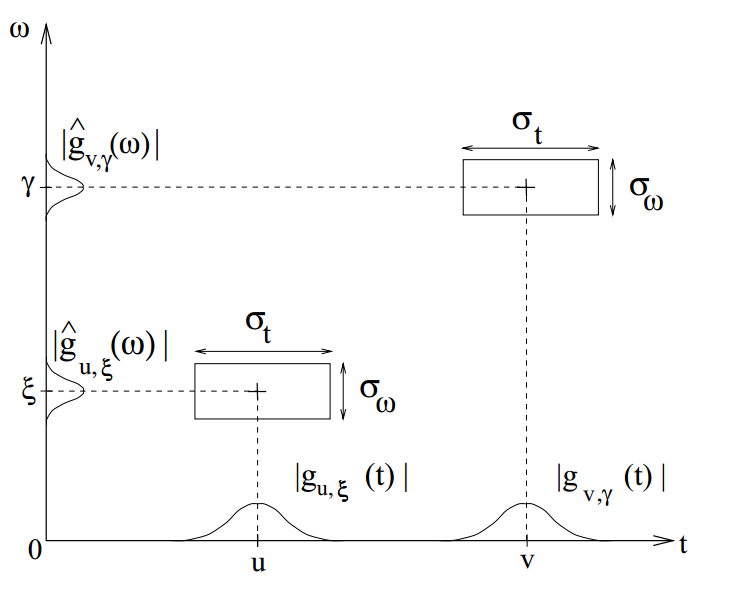
\includegraphics[width=80mm]{LitRev_HeisenbergBox_STFT.png}
\begin{picture}(0,0)
%\put(-355,120){Frequency}
%\put(-200,0){Time}
\end{picture}
\caption{An example of the Heisenberg box illustration and the inherent time-frequency resolution trade-off for the STFT.}
\label{fig:LitRev_HeisenbergBox_STFT}
\end{figure}

In practice this gives rise to a trade-off between temporal and frequency resolution, illustrated in Figure~\ref{fig:LitRev_STFTlims}, where two different temporal frame sizes are shown in relation to the resulting frequency resolution.

\subsubsection{Wavelet decomposition}
The Wavelet Transform can be seen as a generalization of the windowed Fourier transform in that it decomposes a signal over dilated and translated wavelets. A wavelet is simply a function $\phi \in \mathbf{L^2}(\mathbb{R})$ which is normalised $\| \phi \| = 1$, centered in the neighborhood of $t=0$, and with zero average:

\begin{equation}\label{eq:Mallat1999_4}
\int^{+\infty}_{-\infty} \psi(t) dt = 0.
\end{equation}

Unlike the windowed Fourier transform the family of time-frequency wavelet atoms is translated by $u$ as well as scaled by $s$:

\begin{equation}\label{eq:Mallat1999_5}
\phi_{i,s}(t) = \frac{1}{\sqrt{s}}\psi\left(\frac{t-u}{s}\right).
\end{equation}

Now we have that the wavelet transform of $f \in \mathbf{L^2}(\mathbb{R})$ at time $u$ and scale $s$ is

\begin{equation}\label{eq:Mallat1999_x}
W f(u,s) = \langle f, \psi_{u,s} \rangle = \int^{+\infty}_{-\infty} f(t) \frac{1}{\sqrt{s}}\psi^\ast \left( \frac{t-u}{s} \right) dt.
\end{equation}

The energy spread of a wavelet time-frequency atom $\phi_{u,s}$ corresponds to a Heisenberg box centered at $(u,\eta/s)$ where $\eta$ is the center frequency of $\hat{\phi}$ the Fourier transform of $\phi$, and $\hat{\phi_{u,s}}$ is the Fourier transform of $\phi$ dilated by $1/s$. For more details on the derivation of the time-frequency resolution of the wavelet transform see Appendix~\ref{ap:TimeFreqResolutionWavelet} on page~\pageref{ap:TimeFreqResolutionWavelet}. The Heisenberg box remains of area $\sigma_t \sigma_\omega$ at all scales but it is now $s\sigma_t$ on the time axis and $\sigma_\omega /s$ along the frequency axis\cite{Mallat1999}. The temporal and frequency resolution is now dependent on $s$ as illustrated in Figure~\ref{fig:LitRev_HeisenbergBox_wavelets}

\begin{figure}[!] %LitRev_HeisenbergBox_wavelets
\centering
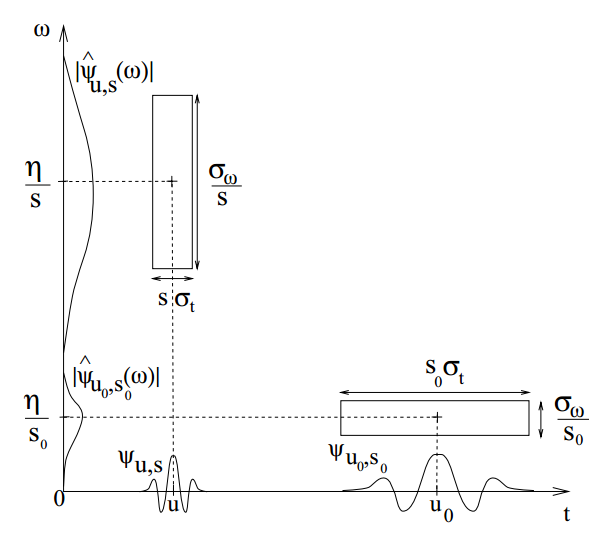
\includegraphics[width=80mm]{LitRev_HeisenbergBox_wavelets.png}
\begin{picture}(0,0)
%\put(-355,120){Frequency}
%\put(-200,0){Time}
\end{picture}
\caption{The Heisenberg boxes for the wavelet transform.}
\label{fig:LitRev_HeisenbergBox_wavelets}
\end{figure}

The main difference between classic Fourier analysis and Wavelet analysis is that Wavelets are localised in both frequency and time whereas the Fourier transform is only localised in frequency. This leads to some significant advantages when considering data that is inherently transient. While the Short Time Fourier Transform (STFT) does, to an extent, mimic the time localisation of the Wavelet Transform it does so at the cost of temporal resolution\cite{Mallat1999}. This inherent trade-off between temporal and frequency resolution is illustrated in Figure~\ref{fig:LitRev_STFTlims} where two different temporal frame sizes are shown in relation to the resulting frequency resolution.

%LitRev_STFTlims
\begin{figure}
\centering
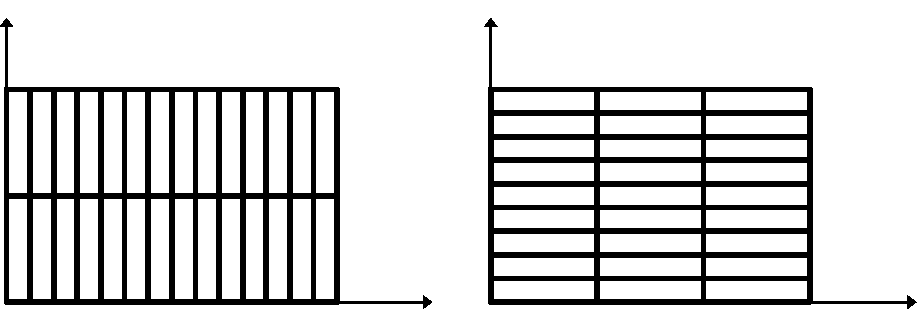
\includegraphics[width=120mm]{LitRev_STFTlims.pdf}
\begin{picture}(0,0)
\put(-355,120){Frequency}
\put(-200,0){Time}
\put(-175,120){Frequency}
\put(-20,00){Time}
\end{picture}
\caption{Heisenberg boxes of two wavelets. At larger scales the frequency resolution is increased by a decreased frequency support and the time spread is increased.}
\label{fig:LitRev_STFTlims}
\end{figure}

%LitRev_Wavelets
\begin{figure}
\centering
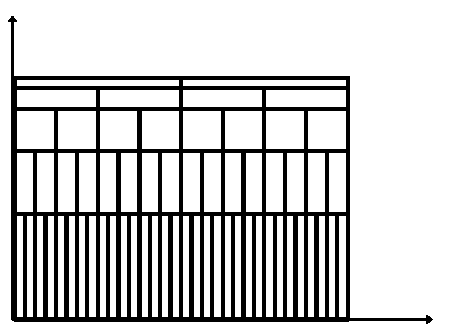
\includegraphics[width=65mm]{LitRev_Wavelets.pdf}
\begin{picture}(0,0)
\put(-195,133){Scale}
\put(-22,-7){Time}
\end{picture}
\caption{The scale-time relationship for the wavelet transform.}
\label{fig:LitRev_Wavelets}
\end{figure}

Figure~\ref{fig:LitRev_Wavelets} shows a similar plot to Figure~\ref{fig:LitRev_STFTlims} but for the Wavelet transform instead. It should be noted that a Wavelet spectrum, equivalent to a traditional spectrogram, is traditionally plotted in the time-scale space, where scale can be seen as being inversely proportional to frequency.

\subsubsection{Multi-resolution analysis with Filter Banks}
Consider now the discrete power spectral density calculation, from Equation~\ref{eq:Mallat1999_3}, for the signal $x(n)$:

\begin{equation}\label{eq:LitRev_Detection_PSD1}
S_{xx}(\omega) = \frac{1}{N} \left| \sum^{N}_{n=1} x(n) e^{-i \omega n} \right|^2.
\end{equation}

For a given frequency $\omega_i$, equation~\ref{eq:LitRev_Detection_PSD1} can be rewritten as

\begin{equation}\label{eq:LitRev_Detection_PSD2}
S_{xx}(\omega_i) = \left\| \sum^{N}_{k=1} h_i(k) x(n-k) \right\|^2,
\end{equation}

where

\begin{equation}\label{eq:LitRev_Detection_PSD3}
h_i(k) = w(k)e^{-i \omega_i n},
\end{equation}

and $w(k)$ is a window function. Considering $w(k)$ as a prototypical FIR lowpass filter, the collection of all $h_i(k)$s constitutes a bank of bandpass filters each centered on frequency $\omega_i$\cite{Ariananda2013}. This implementation is commonly referred to as the periodogram but it also highlights what sometimes is called the filter bank paradigm and is a particularly simple implementation of the DWT\cite{Mallat1999}.

Considering again the window function $w(k)$ from equation~\ref{eq:LitRev_Detection_PSD3}, the simplest window conceivable would be a simple rectangular window $w(k) = 1/N$. Naturally this would lead to significant side lobe leaks in the spectral domain and is therefore highly undesirable. Employing Hamming and Hann windows is a common approach to alleviate these issues. Another issue that arises with the periodogram is that its estimates are coarse with low precision and large variance\cite{Ariananda2013}. A common method for alleviating this variance problem is by windowing the data first\cite{Lim1988book}.

Work done on Multi Taper Spectrum Estimation (MTSE)\cite{Thomson1982} and later on multi-resolution theory\cite{Mallat1989}\cite{Meyer1995} proves that conjugate mirror filter characterizes a wavelet and that cascading these filters will lead to a fast implementation of the discrete wavelet transform.

Figure~\ref{fig:LitRev_DWTstep.pdf} shows a diagrammatic representation of a single step of the DWT. The \emph{Lo} and \emph{Hi-pass} filters represent, respectively, the low and high pass conjugate mirror filters and the following step is a dyadic decimation (down-sampling) step. Since the spectrum of each filtered signal is effectively halved by the filters, the decimation step removes redundant information in accordance with Nyquist's theorem. The output of the low and high-pass filters are commonly referred to as the approximation and the detail coefficients respectively\cite{Mallat1999}.

%LitRev_DWTstep.pdf
\begin{figure}
\centering
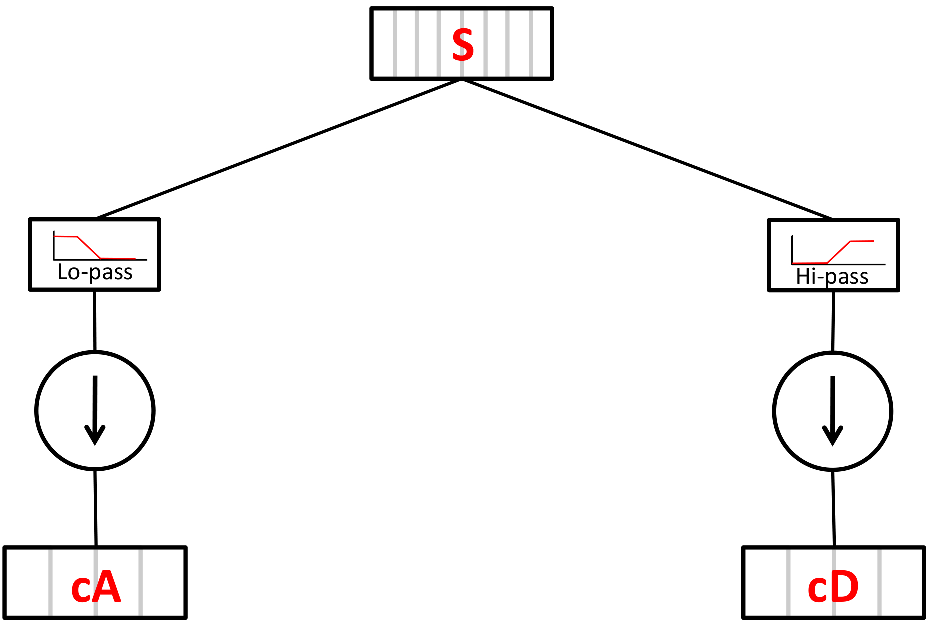
\includegraphics[width=85mm]{LitRev_DWTstep.pdf}
\begin{picture}(0,0)
%\put(-195,133){Scale}
%\put(-22,-7){Time}
\end{picture}
\caption{A single wavelet decomposition step.}
\label{fig:LitRev_DWTstep.pdf}
\end{figure}

Figure~\ref{fig:LitRev_DWTtree.pdf} shows a three level wavelet decomposition.
%LitRev_DWTtree.pdf
\begin{figure}
\centering
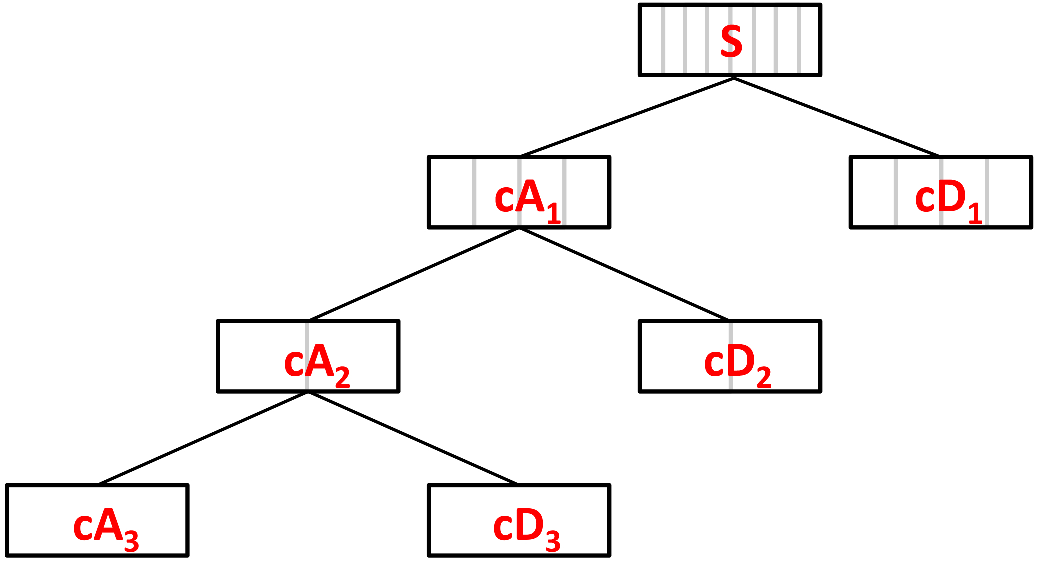
\includegraphics[width=85mm]{LitRev_DWTtree.pdf}
\begin{picture}(0,0)
%\put(-195,133){Scale}
%\put(-22,-7){Time}
\end{picture}
\caption{Three level wavelet decomposition tree.}
\label{fig:LitRev_DWTtree.pdf}
\end{figure}

The multi-resolution properties of the wavelet transform has made the Wavelet transform popular in a range of audio and speech applications where much of the information of interest is located in the lower frequency bands\cite{Sinha1993}\cite{Czyzewski1995}\cite{Lambrou1998}\cite{Biscainho2000}\linebreak[0]\cite{Tzanetakis2001}\linebreak[0]\cite{Zurera2001}\cite{Lin2005}\cite{Nongpiur2008}. Equally the computational efficiency of the discrete wavelet transform is cited\cite{Kadambe1992} as a significant advantage over the FFT with an $O(N)$ complexity compared to\linebreak[0] $O(N\mathrm{log}(N)$ for FFT\cite{Mallat1999}. In \cite{Kadambe1992} the authors report ``superior pitch detection performance'' citing the Wavelet transforms computational efficiency, temporal resolution and its suitability of the pitch periods found in the analysed material. Speech applications in particular report good spectral estimation capabilities \cite{Hu2004}, good de-noising capabilities \cite{Donoho1995}\cite{Seok1997}, and good compression performance \cite{Sinha1993}\cite{Fgee1999}. Several authors propose wavelets used as a bases for audio classification applications\cite{Lambrou1998}\cite{Tzanetakis2001}\cite{Lin2005} and report that a specific advantage of the wavelet basis is its compact representation compared to the time domain signal which decreases processing delay/cost\cite{Lambrou1998}.

An early wavelet based click detection algorithm proposes to detect clicks by analysing the wavelet coefficients of the signal for discontinuities\cite{Czyzewski1995}. The authors apply a neural network algorithm to robustly detect and classify pulses although the authors note that the required training stage is both ``a complex and time-consuming procedure''. While not explicitly discussed the authors appear to be targeting extremely short time pulses of the order of 1 or 2 samples, or what they call ``parazite impulses''.

More recently the wavelet bases has been used to detect impulsive noise in speech data by taking advantage of the relatively slow time-varying nature of speech and the Lipschitz regularity of the speech components\cite{Nongpiur2008}. For this application the scope of the corrupted samples appeared larger with suggested possible corruptions including gunshots, rain drops and keyboard typing noise. The author reported that the algorithm managed to reduce the rain drop noise in an instantaneous mixture of speech and rain noise. It was noted that this was the only noise application demonstrated and that it was never intended to completely remove the noise entirely. It is also noted that additional noise suppression algorithms seems to have been used as well as a speech enhancement algorithm. The extent to which this algorithm would reduce the nuisance of longer and louder pulses would have been interesting.

\subsubsection{Wavelet Packet Transform (WPT)}
The Wavelet Packet Transform (WPT) can be seen as a generalisation of the Wavelet transform in that it extends the link between multi-resolution approximations and wavelets. The WPT can also be seen as a natural extension of MSTE\cite{Thomson1982}. While the DWT decomposes only the approximation coefficients the WPT applies the decomposition step symmetrically throughout the tree as seen in Figure~\ref{fig:LitRev_WPTtree.pdf}. Since the standard DWT algorithm is limited to wavelet bases that increase by a power of two towards the higher scales (low frequencies) it is possible that some other combination of bases could provide a better basis in some applications\cite{Coifman1992a}.

%LitRev_WPTtree.pdf
\begin{figure}
\centering
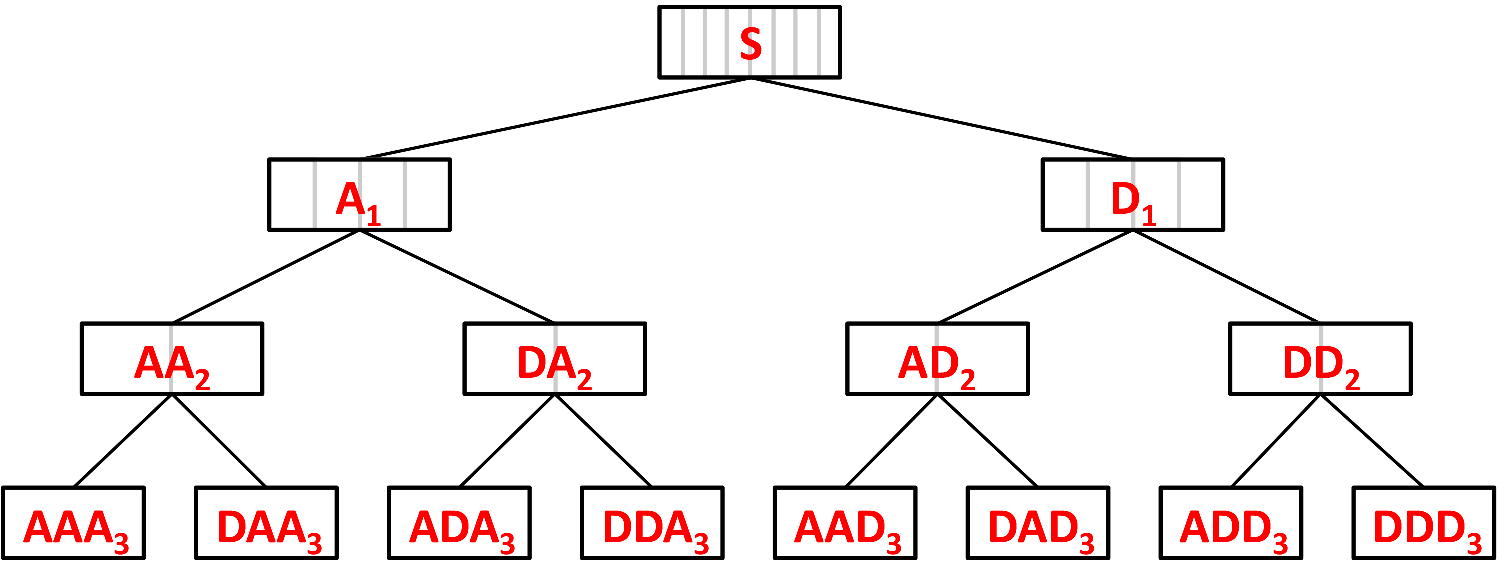
\includegraphics[width=125mm]{LitRev_WPTtree.pdf}
\begin{picture}(0,0)
%\put(-195,133){Scale}
%\put(-22,-7){Time}
\end{picture}
\caption{Three level wavelet packet decomposition tree.}
\label{fig:LitRev_WPTtree.pdf}
\end{figure}

In a recent study comparing the WPT to other spectrum estimation techniques it was generally found that the WPT ``operated well for all types of sources and its performances were comparable or at times even better than other existing \linebreak[0]approaches.''\cite{Ariananda2013}. In particular it was found that WPT performed well in reducing variance in the stop bands.

The authors of \cite{He2008} developed a psychoacoustic model based around the WPT and found that not only was the WPT computationally more efficient than a Fourier transform-based alternative but it also provided a better spectral resolution. For psychoacoustic applications it was found that the generalization of the DWT yielded a better approximation of the critical bands employed\cite{Carnero1999}\cite{He2008} compared to similar DWT based models\cite{Sinha1993}\cite{Zurera2001}.

\section{Restoration}\label{sec:LitRev_Restoration}
The restoration of corrupted speech and audio samples by a localised degradation, also referred to as clicks or noise pulses, has inspired much research and many approaches. Corruptions can generally be seen to have varying severity. Clicks and pulses have traditionally been treated as completely corrupted or essentially missing samples transforming the restoration task into one of interpolation of missing samples\cite{Tukey1974}\cite{Tukey1977}\cite{Godsill1998book}.

An exhaustive review of the methods employed in the field up until the year of publishing in 1992 can be found in \cite{Veldhuis1992}. A summary of relevant methods and more recent methods are provided in this section. While the focus of this thesis is the interpolation of audio segments, as with the detection task, some methods or related approaches can be found in the field of image restoration of localised corruptions or other 1 and 2 dimensional implementations.

\subsection{Nonlinear approaches}\label{sec:LitRev_RestorationNonLin}
As noted in section~\ref{sec:LitRevDetMedianFilts}, a classic pulse detection approach in both audio and image processing has been by median filtering. Equally, many of the approaches mentioned previously employ median based approaches for restoring the detected pulses\cite{Tukey1974}\cite{Lee1985}\cite{Heinonen1985}\cite{Heinonen1987}\cite{Maekivirta1991}\cite{Kasparis1993}\cite{Alajlan2004}. In \cite{Bovik1983} it was shown that the optimal Order Statistics Filter (OSF) tends towards a median filter as the noise becomes increasingly impulsive, and that in particular the median filter is effective when the pulse length is less than half the median window size\cite{Alajlan2004}.

Much of the early work on nonlinear digital smoothing followed the original proposed algorithm by Tukey\cite{Tukey1974}. Following this publication the algorithm, in combination with linear filtering, was applied to speech signals and was found to perform reasonably\cite{Rabiner1975}. The authors noted that the median filter alone, although successful in the preservation of sharp discontinuities not associated with noise, failed to provide sufficient smoothing and was therefore paired with a simple 3-point linear filter. In addition the authors described a double smoothing algorithm which attempted to isolate noisy segments and re-subtract them.


%Median filtering for restoration:
%JAYNAT, N.S.: ‘Average and median based smoothing for improving
%digital speech quality in the presence of transmission errors’,
%IEEE Trans., COM-24,1976, pp. 1043-1045
%\cite{Jayant1976}
%
% ^ Efficacy of employing some simple waveform smoothing. Transmission errors.
%
A similar early approach used to combat the effects of transmission errors in digital speech signals employed simple waveform-smoothing techniques and reported a ``cleaner-sounding'' speech in the presence of ``fairly significant'' error rates\cite{Jayant1976}. The result of this was unfortunately also a smearing of the speech component but the authors found that for high probability of errors this pulse-squelching operation was still perceptually desirable in spite of speech smearing. These results were backed up by a six person subjective study.

\todo{Add this reference in!}
%RABINER, L.R., SAMBUR, M.R., and SCHMIDT, C.Es
%of a nonlinear smoothing algorithm to speech processing.
%IEEE Trans., ASSP-32, (3), 1975
\cite{Rabiner1975}
%
% ^ Median and linear smoothing combined.
%   Linear smoothing is rarely enough.
%
% "Generalized median filtering and related nonlinear filtering techniques"
% Another median+linear smoother

These methods all appear to have been applied indiscriminately to the data sequences which bore a cost to the signal fidelity.

%Median LPC hybrid
%NIEMINEN, HEINONEN, P., and NEUVO, Y.: ‘Suppression
%and detection of impulsive type interference using adaptive median
%hybrid filter’. IEEE Proc. ICASSP 1987, pp. 117-120.

Realizing the power of both linear and non-linear approaches to non-stationary noise detection and restoration, a range of \emph{hybrid} approaches arose\cite{Nieminen1987a}\cite{Lee1985} \cite{Heinonen1987}. A Modified Trimmed Mean (MTM) filter, was found to outperform a standard median filter in the task of preserving naturally sharp edged in signals\cite{Lee1985}. The MTM filter quite simply replaces values of a frame with the average of a subframe selected around the outer frame's median value\cite{Lee1985}. An FIR Median Hybrid (FMH) filter was designed with the aim of outperforming the standard median filter computationally. The FMH filter was found to perform similarly the the standard median filter\cite{Heinonen1987}. Lastly the Adaptive Median Hybrid (AMH) filters, proposed in \cite{Nieminen1987a}, employ multiple substructures which was considered ``ideal for processing of signals with statistics which change abruptly''. The theory is that at least one of the substructures will have adapted to a local change in the signal characteristics, whereas short non-stationary changes will be omitted. For the examples presented, this approach conserved sharp local changes while a comparable Least Means Squares (LMS) filter did not\cite{Nieminen1987a}.

From a computational perspective median filters involve a sequence of searching and sorting steps and despite dedicated hardware for these operations these procedures are generally computationally intensive\cite{Kundu1984}. A generalised mean implementation for black and white photos showed similar, and in some cases better, performance to the median filter while maintaining a distinct computational advantage\cite{Kundu1984}.

%Lee: L and M filters + useful modification: MTM filter
% "combine properties of both the linear and median filters"
% "The concept of double-window filtering is introduced as a refinement of MTM filtering"
% "It was observed that M filters offers a more favorable combination of the characteristics of running mean and median filters than the L filters"
% "The MTM filters were shown to provide better overall characteristics. In fact, we have seen that MTM filters can preserve noisy edges better than can median filters."

%Heinonen: FIR-median hybrid (FMH) filters (M filter)
% "The FIR-median Hybrid (FMH) filters require significantly less computations than the Standard Median (SM) filters.

%Nieminen: Adaptive Median Hybrid (AMH) filters
% "In the AMH filters, adaptive filter substructures are used
% to estimate the current signal value from the future and
% past signal values. The output of the overall filter is the
% median of the %adaptive filter outputs and the currents ignal
% value. This kind of nonlinear filter structure is shown to
% adapt and preserve rapid changes in signal characteristics
% well. However, it filters out short duration interferences. By
% examining the difference between the original and filtered
% data, interferences can be detected."

% Non-linear, minimum or maximum of neighborhood based on dark or bright spot. (Alajlan based on Windyga, good explanation of Windyga in Alajlan)
In the field of image processing the median filter is still an integral part in most state-of-the-art impulsive noise filters\cite{Alajlan2004}. Other popular non-linear methods employed have been the maximum-minimum method\cite{Xu1998} and the peak-and-valley filter\cite{Windyga2001} and a modified maximum-minimum approach\cite{Alajlan2004} which aims apply a maximum-minimum approach to selected samples only. All these non-linear approaches were found to have similar performance but with median filter bearing a higher computational cost\cite{Alajlan2004}.

% waveform substitution schemes
%\cite{Goodman1986}\cite{Wasem1988}\cite{Niediwiecki2001}
A more direct and heuristic approach to waveform and audio restoration of longer gaps is found in waveform substitution\cite{Goodman1986} or ``smart copying''\cite{Niediwiecki2001}. An audio segment immediately prior to a corruption is used as a template for finding a segment earlier in the segment which matches it. It is assumed that what follows the best match for the template will be a good substitute for the corrupted segment. Given that speech signals ``display quasi-stationary intervals''\cite{Goodman1986} this algorithm produces feasibly looking results given that the corruption does not straddle regions with high-energy voiced speed, low-level unvoiced speech or silence\cite{Goodman1986}. Waveform substitution has been confirmed through several objective listening tests to have ``satisfactory'' results\cite{Niediwiecki2001}. In addition the method excels by being computationally simple\cite{Niediwiecki2001}.

%pitch detection
An extension of the basic waveform substitution algorithm an additional pitch detection extension was proposed. If a pitch estimate is available the pitch period prior to the corruption may be reproduced throughout the corruption\cite{Goodman1986}. No direct results were presented to quantify the performance of this addition but a later publication ranks a pitch waveform replication algorithm as the producing the highest quality results based on subjective tests\cite{Wasem1988}. In this test the method was compared with a simple silence insertion and packet repetition algorithms suffering from obviously audible discontinuities\cite{Goodman1986} in addition to one and two-sided waveform substitution algorithms\cite{Goodman1986}. It was noted that while the pitch waveform replicator produced the highest quality results it was not the most computationally complex nor did it produce the longest delays of the tested algorithms\cite{Wasem1988}.

A similar heuristic pitch based approach proposes to model speech as a series of spectral peak tracks that are ``born'' and ``die'' employing the short time Fourier transform (STFT)\cite{Maher1994}. First proposed be \cite{McAulay1986} this method has since then been referred to as MQ representation (after the authors' names) and been applied to the task of speech interpolation\cite{Maher1994}. Many other authors have applied sinusoidal models for speech modeling in a variety of applications\cite{Godsill1998book}\cite{Vera-Candeas2003}\cite{Wells2006} which attempts in some cases to generalize the glottal excitation model in speech\cite{McAulay1986}.
%other sinusoidal based approaches

% P. A. A. Esquef, L. W. P. Biscainho, V. Välimäki, and M. Karjalainen, "Removal of Long Pulses from Audio Signals Using Two-pass Split-Window Filtering", presented at the 112th AES Convention, preprint no. 5535, Munich, Germany, May 10-13, 2002. \cite{Esquef2002a}

\subsection{Linear approaches}\label{sec:LitRev_RestorationLin}
%Skip
% Band limited extrapolation/band-limited interpolation
%\cite{Papoulis1975}\cite{Ferreira2001}

In speech signals a popular and successful method of interpolation is the autoregressive (AR) approach\cite{Vaseghi1988thesis}\cite{Godsill1998book}\cite{Kauppinen2002b}. An early approach using this method demonstrated that this method produced satisfactory results for specifically speech signals, based on both objective and subjective results, and furthermore established the feasibility of real-time implementation of such methods\cite{Janssen1986}. Independent development applied the methods to audio restoration applications\cite{Vaseghi1988thesis}\cite{Vaseghi1990}.

Typically longer stretches of audio interpolation has been difficult applications for AR models\cite{Veldhuis1992}\cite{Kauppinen2002b}, but modified AR based models have been applied to the pure extrapolation problem with some success to longer gaps\cite{Kauppinen2002b}. The basic AR models, and later least squares (LS) AR extensions\cite{Godsill1998book}, have also been paired with synthesis filters designed to excite the AR model to achieve longer gap extrapolation with lower model orders\cite{Esquef2006}. This method achieves comparable perceptual quality to higher order AR models given significantly lower model complexity\cite{Esquef2006}.

In general many authors have considered linear predictive coding (LPC) and AR models for audio and speech data\cite{Vaseghi1990}\cite{Czyzewski1995}\cite{Godsill1998}. A more comprehensive review of AR, LPC and warped-based methods were covered in section~\ref{sec:LitRevAR} from the perspective of modeling speech and audio in the detection application.

%An Efficient Model-Based Method for Reconstruction of Audio Signals Across Long Gaps
%\cite{Esquef2006} (based on \cite{Kauppinen2002a} and \cite{Kauppinen2002b})
% The use of a maximally-decimated filterbank renders easier
%the interpolation task within a subband. This is due to the decreased
%number of resonance modes to be modeled, allowing
%model order reduction. In addition, the length of the gap to fill
%in shortens by the decimation factor of the subband. For the two
%lowest subbands this factor is 1/32.
%
%In such situations AR-based interpolators tend to perform poorly toward the middle of the gap, where the energy of the
%interpolated signal decreases [13].
%The aforementioned signal energy reduction occurs in part
%due to the minimization of the AR modeling error, which is employed
%to solve for the unknown samples within a given gap
%[15]. In the ideal case of a null modeling error, the resulting interpolated
%signal would be determined mainly by the impulse
%response of the AR model.%


%\cite{Vaseghi1990}: LPC. "An interpolation algorithm was
%described that takes advantage of the quasi-periodic
%nature of glottal excitation and provides better estimates
%than the existing method."

% interpolators based on sinusoidal modeling
%\cite{Maher1994}\cite{Godsill1998book}

% subband methods
%\cite{Montresor1991} \cite{Cocchi2001}

%Low frequency pulse corruption:
%|P. A. A. Esquef, L. W. P. Biscainho, and V. Välimäki, "An Efficient Algorithm for the Restoration of Audio Signals Corrupted with Low-Frequency Pulses", Journal of the Audio Engineering Society, vol. 51, no. 6, pp. 502-517, June 2003
%\cite{Esquef2003a}

%Wavelet Shrinkage:
%|L. W. P. Biscainho, F. P. Freeland, P. A. A. Esquef, and P. S. R. Diniz, "Wavelet Shrinkage De-noising Applied to Real Audio Signals under Perceptual Evaluation," in Proc. X European Signal Processing Conf. (EUSIPCO 2000), pp. 2061-2064, Tampere, Finland, September 2000.
%\cite{Biscainho2000}

%

%\subsection{Median filtering}

%\cite{Nongpiur2008} : "On the basis of these differences, an algorithm was developed
%to identify and suppress wavelet coefficients that correspond to
%impulse noise."

% A comprehensive review of restoration methods can be found in \cite{Veldhuis1992}

%\section{Residual Restoration}
%A variety of restoration algorithms have been tested for the restoration of the residual audio component. Based on the nature of the detection algorithm, the restoration step can be done either on the wavelet coefficients or on the time series data.

\todo{something more}



% ------------------------------------------------------------------------


%%% Local Variables:
%%% mode: latex
%%% TeX-master: "../thesis"
%%% End:




\chapter{Acoustic Pulse Recognition System}\label{ch:APR}

\ifpdf
    \graphicspath{{Chapter3_APR/Chapter3Figs/PNG/}{Chapter3_APR/Chapter3Figs/PDF/}{Chapter3_APR/Chapter3Figs/}{Chapter3_APR/Chapter3Figs/PDF/}{Chapter3_APR/Chapter3Figs/Kamplitude/}}
\else
    \graphicspath{{Chapter3_APR/Chapter3Figs/EPS/}{Chapter3_APR/Chapter3Figs/}}
\fi

This chapter describes work undertaken with several waveform classification algorithms, specifically designed to detect and classify taps incident on a device containing a single microphone. The different models in the classification algorithms correspond to different tapping positions $j$ on the device, and the algorithms can therefore be said to represent a new touch screen technology using \gls{apr}. This chapter is specifically focussed on applications using a single sensor to attempt to tackle the difficult issue of the structural uncertainty and its effect on recorded waveforms without the aid of inter microphone time and intensity differences.

Traditionally the given data in selection problems have been referred to as models. In the following section these models will occasionally be referred to as templates in the context of the specific models for this application.

\section{Background}
Modern touch screen devices have, generally speaking, 2 main attributes. Firstly they function without the need for any additional interfacing hardware and secondly they let a user interact directly with the data presented to the user. The methods introduced in the following sections attempt to reconcile these attributes with factors such as scalable deployment and low manufacturing, and implementation costs through \gls{apr}.

The underlying assumption of an \gls{apr} system is that tapping on any spot, on the touch sensitive surface, creates a unique acoustical pulse, that this unique pulse is largely reproducible and that it is detectable. Figure~\ref{fig:twotwoSampleTap} shows a plot of 4 tap pulses recorded at 2 different spots on the device. It is seen from the plot that tapping in these two different locations produces noticeably different pulses and that the pulses from the same spot are, though slightly different in certain parts of the signal, still visibly similar. The 4 taps in Figure~\ref{fig:twotwoSampleTap} have been aligned to the onset of the tap.

\begin{figure}[t]
  \begin{center}
    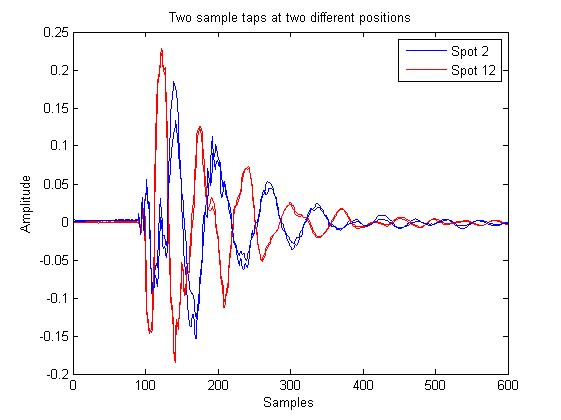
\includegraphics[width=110mm]{twotwoSampleTap}
    \caption{Two taps recorded at both spot 2 and 12 (refer to Figure~\ref{fig:phoneDisplayNum} for spot location). Sampled at 44.1 kHz.}\label{fig:twotwoSampleTap}
  \end{center}
\end{figure}

%Maybe not use this paragraph... rewrite at least.
Although Figure~\ref{fig:twotwoSampleTap} shows the scope of the variability in the pulses due to impact site, it is worth recognizing that this variability is fairly modest compared to the variability observed when comparing tapping pulses with data such as speech or even other percussive signals. It is also worth noting that some variability arises from certain environmental conditions, so the nature of the problem can be summed up as being one where certain variations are expected and others are used as the basis for classification.

\section{System}\label{sec:APRsystem}
The system developed consists of a number of different elements that crudely can be divided into hardware and software. The hardware system can be considered as a testing rig for the algorithm and is designed to facilitate a single output, black box type, approach to the classification problem, where the black box represents a unknown complex vibrational system with certain transfer characteristics. These characteristics are assumed to be reproducible or time-invariant. Figure~\ref{fig:blackBox} represents such a system, where $x^j$ can be considered some pulse on a spot $j$ known by the user, while $y$ is the output of the black box as seen by the classification algorithm oblivious to the origin of the tap $j$.

\begin{figure}[!]
\centering
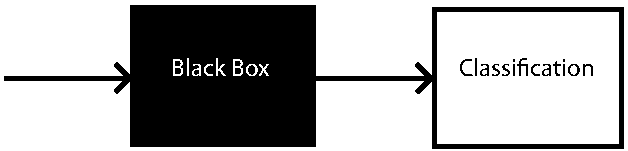
\includegraphics[width=100mm]{blackBox.pdf}
\caption{Black box representation of structural uncertainty in a tapping device.}\label{fig:blackBox}
\begin{picture}(0,0)
\put(-120,83){$x^j$}
\put(22,83){$y$}
\end{picture}
\end{figure}

Two pieces of hardware were produced to achieve these characteristics. Firstly a mobile phone implementation of the algorithm was considered and an actual mobile phone handset was acquired and modified to allow for external analogue monitoring of the internal microphone. The mobile phone chosen for this application was a Samsung SGH-M150, which can be seen in Figure~\ref{fig:phone}. This device was chosen based on its ability to be easily modified to allow for external interfacing with the microphone. Additionally a grid of $J = 12$ points was added to the screen area as reference points for tapping.

\begin{figure}[!]
\centering
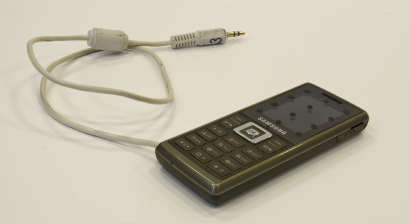
\includegraphics[width=410 px]{phone.png}
\caption{Picture of modified Samsung SGH-M150 mobile phone with 12 spot grid on display area.}\label{fig:phone}
\end{figure}

A larger application of the same black box characteristics is a simple wooden board, measuring $30.6 \times 24.3 \times 1.8$ cm (l$\times$w$\times$d), with a grid of 30 spots marked on the face of it. Attached on the back of the board, in a small cavity, is a microphone to pick up an acoustic signal from the board when tapped.  The board can be seen in Figure~\ref{fig:Pad}. The microphone used for this application is a DPA Microphone 4060 omnidirectional condenser microphone. This microphone was chosen for its excellent linear characteristics, its high sensitivity and dynamic range.

\label{corrections:wooden}While the wooden board does not actually contain a screen it is noted that the screen functionality is not required for the \gls{apr} technology to work. In essence the wood could be replaced by a screen, and although it would certainly have very different vibrational characteristics than an actual screen, these differences may not actually matter. It is also noted that any object can be considered a screen as long as an image is projected onto it.

\begin{figure}[!]
\centering
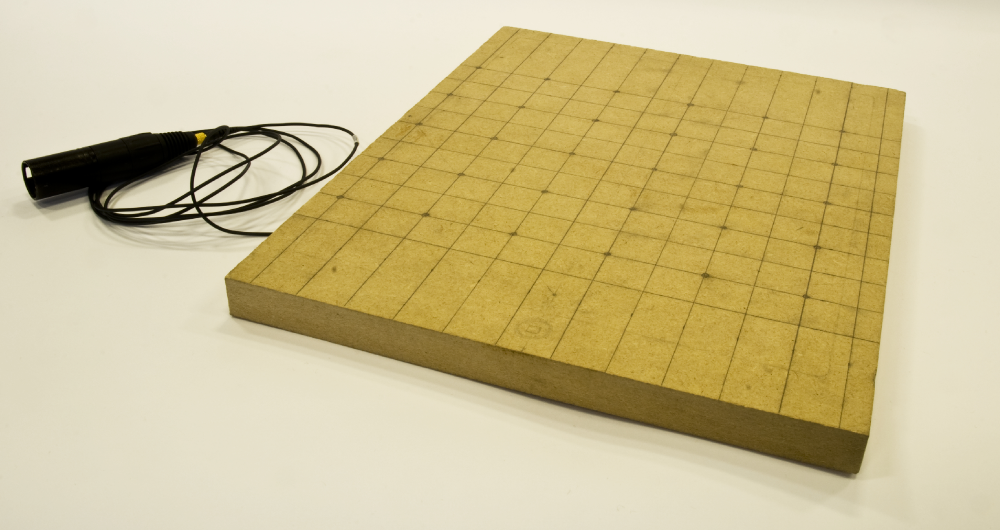
\includegraphics[width=410 px]{Pad.png}
\caption{Picture of wooden board with attached microphone to the back and 30 spot grid on the front.}\label{fig:Pad}
\end{figure}

The second part of the system is the software. Figure~\ref{fig:system} shows a simple block diagram representing the system where the bottom row is meant to represent the software system. The display on this figure represents the output from the interpolation extension to the \gls{ml} and \gls{map} methods, described later in the chapter. In this system definition, the hardware can be viewed as being the ``restricting'' factor while the software is the ``redeeming'' factor, and hence the attention is now turned to the models and algorithms of the system.

\begin{figure}[!htbp]
  \centering
    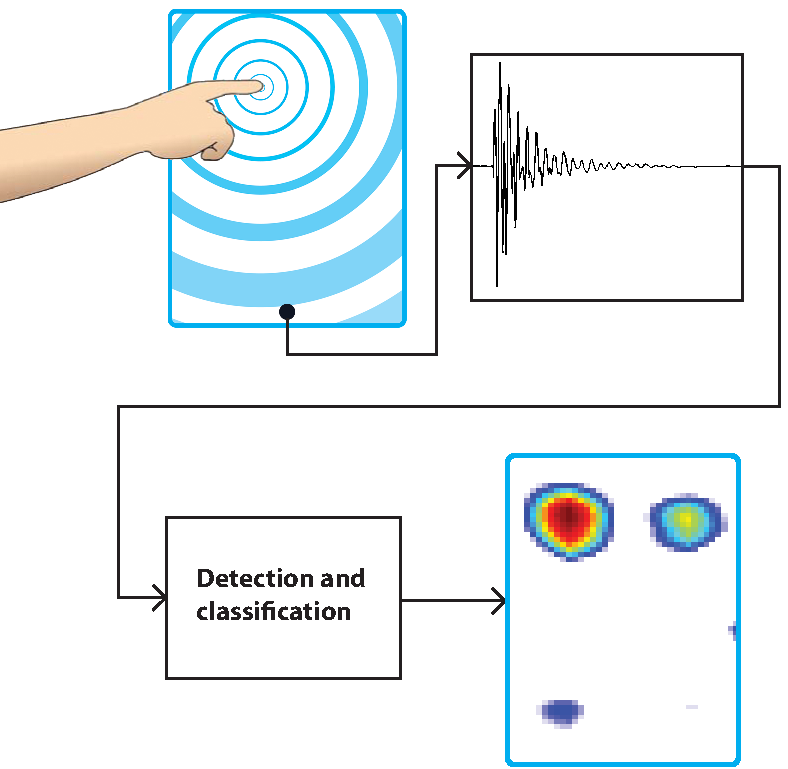
\includegraphics[width=110mm]{system.pdf}
    \caption{Block diagram of detection system. The display displays an intensity map of likelihoods superimposed on the device, as described in the extension to the \gls{ml} and \gls{map} methods.}\label{fig:system}
\begin{picture}(0,0)
\put(-136,239){Microphone}
\put(-57,179){DSP}
\put(72,204){Display}
\put(50,364){Tapping pulse}
\put(-72,243){\vector(2,1){25}}
\end{picture}
\end{figure}

\section{ML and MAP methods}
\subsection{Model and theory}
Suppose that each data reading $y = [y_0, \ldots , y_{N-1}]^T $ is modeled by the linear model

\begin{equation}\label{eq:MLmod1}
y = \theta^j t^j(n_0) + v,
\end{equation}
where $t$ is a set of $J$ templates, of length $M$, from $J$ different spots so that $t^j(n_0)$ is then the $j$th template, $j \in \{1, \ldots ,J\}$ shifted to time $n_0$ and $\theta$ is taken to be a random variable describing the scaling of the template. The prior on $\theta$ is assumed to be normal and independent across $j$.
\begin{equation}\label{eq:MLtheta}
\theta^j \sim \mathcal{N}(\mu^j_{\theta},\sigma_{\theta,j}^2),
\end{equation}

and $v$ is the independent and identically distributed (i.i.d.) Gaussian noise, modeling the background interference:

\begin{equation}\label{eq:MLnoise}
v \stackrel{i.i.d.}{\sim} \mathcal{N}(0,\sigma^2).
\end{equation}

Templates $t^j(n_0)$ for which the alignment $n_0$ and length makes them exceed the length of available data $N$, are truncated.

Henceforth the scaling factor $\theta^j$ and template $t^j(n_0)$ will be referred to respectively as $\theta$ and $t$ for simplicity.

To evaluate which, if any, of the templates are present in the data and when they are observed we need to evaluate the probability of the template number $j$ and the time shift $n_0$ given the received data $y$ which can be described as $p(j,n_0|y)$.

Using Bayes' theorem it is found that:

\begin{equation}\label{eq:MLBayes}
p(j,n_0|y) \propto p(y|j,n_0)p(j,n_0),
\end{equation}

where $p(j,n_0|y)$ is the posterior probability, $p(y|j,n_0)$ is the likelihood and $p(j,n_0)$ is the prior probability.
Take the prior probability to be:

\begin{equation}\label{eq:MLPrior}
p(j,n_0) = \frac{1}{JN},
\end{equation}
as the expression for a non-informative prior, which can be modified with time.
The likelihood can be expressed as the marginalisation of the conditional probability of the data $y$ given the scaling $\theta$, template number $j$ and the time shift $n_0$, over $\theta$, so that:

\begin{equation}\label{eq:MLmargin}
p(y|j,n_0)=\int_\theta p(y|\theta, j, n_0) p(\theta|j,n_0) d\theta,
\end{equation}

where the product of the two normal distributions $p(y|\theta, j, n_0)$ and $p(\theta|j,n_0)$, can be expressed as a third unnormalised normal distribution and a normalising constant $z$.

\begin{equation}\label{eq:MLprod1}
\mathcal{N}_y(\theta t,\sigma^2 \textbf{I})\cdot\mathcal{N}_\theta(\mu_\theta,\sigma^2_\theta) = z \times \mathcal{N}_\theta(\hat{\mu}_\theta,\hat{\sigma}^2_\theta),
\end{equation}
where $\textbf{I}$ is the appropriate $M \times M$ identity matrix and $\mathcal{N}_\theta(\hat{\mu}_\theta,\hat{\sigma}_\theta^2)$ is the third normal distribution which is the only element on the r.h.s. which is dependent on $\theta$,

\begin{equation}\label{eq:MLtheta2}
\mathcal{N}_\theta(\mu_\theta,\sigma^2_\theta) = \frac{1}{\sqrt{2 \pi \sigma_\theta^2}} \textrm{exp}\left[-\frac{\left(\theta - \mu_\theta\right)^2}{2\sigma_\theta^2}\right],
\end{equation}

and

\begin{equation}\label{eq:MLnoise2}
\mathcal{N}_y(\theta t,\sigma^2 \textbf{I}) = \frac{1}{\left(2 \pi\right)^{\frac{M}{2}\sigma}} \textrm{exp}\left[-\frac{\left(y - \theta t\right)^T\left(y - \theta t\right)}{2\sigma^2}\right].
\end{equation}

It is now possible to write the marginalisation in equation (\ref{eq:MLmargin}) as:

\begin{equation}\label{eq:MLmargin2}
p(y|j,n_0)=\int_\theta \mathcal{N}_y(\theta t,\sigma^2 \textbf{I})\cdot\mathcal{N}_\theta(\mu_\theta,\sigma^2_\theta) d\theta = z \int_\theta \mathcal{N}_\theta(\hat{\mu}_\theta,\hat{\sigma}^2_\theta) d\theta = z,
\end{equation}

since $\int_\theta \mathcal{N}_\theta(\hat{\mu}_\theta,\hat{\sigma}^2_\theta) d\theta = 1$.

To evaluate $\hat{\sigma}^2_\theta$ and $\hat{\mu}_\theta$, the l.h.s. of equation (\ref{eq:MLprod1}) must be expanded,

\begin{eqnarray}\label{eq:MLprod3}
& & \mathcal{N}_y(\theta t,\sigma^2 \textbf{I})\cdot\mathcal{N}_\theta(\mu_\theta,\sigma^2_\theta) \\\nonumber{}\\\nonumber
& & \quad = \frac{1}{\left(2\pi\right)^{\frac{M+1}{2}} \sigma \sigma_\theta} \textrm{exp}\left[-\frac{1}{2}\left(\frac{y^Ty +\theta^2t^Tt-2\theta y^T t}{\sigma^2}+\frac{\theta^2 + \mu^2_\theta-2\theta\mu_\theta}{\sigma_\theta^2}\right)\right]\\\nonumber{}\\\nonumber
& & \quad = \frac{1}{\left(2\pi\right)^{\frac{M+1}{2}} \sigma \sigma_\theta} \textrm{exp}\left[-\frac{1}{2}\left(\theta^2 \left(\frac{1}{\sigma_\theta^2}+\frac{t^T t}{\sigma^2}\right) - 2\theta\left(\frac{y^T t}{\sigma^2}+\frac{\mu_\theta}{\sigma_\theta^2}\right) + \frac{y^Ty}{\sigma^2} +\frac{\mu_\theta^2}{\sigma_\theta^2}\right)\right].
\end{eqnarray}

Expanding the r.h.s. of equation (\ref{eq:MLprod1}) gives

\begin{eqnarray}\label{eq:MLprod4}
& & z \times \mathcal{N}_\theta(\hat{\mu}_\theta,\hat{\sigma}^2_\theta) \\\nonumber{}\\\nonumber
& & \quad = \frac{z}{\sqrt{2 \pi}\hat{\sigma}_\theta}\textrm{exp}\left[-\frac{1}{2}\left(\theta^2\frac{1}{\hat{\sigma}^2_\theta} - 2\theta\frac{\hat{\mu}_\theta}{\hat{\sigma}^2_\theta} + \frac{\hat{\mu}_\theta^2}{\hat{\sigma}^2_\theta}  \right)\right]
\end{eqnarray}

By observation between equation (\ref{eq:MLprod3}) and (\ref{eq:MLprod4}) it is found that:

\begin{eqnarray}
\label{eq:MLprod5}
\hat{\sigma}^2_\theta &=& \left(\frac{t^T t}{\sigma^2} + \frac{1}{\sigma_\theta^2}\right)^{-1} \qquad \textrm{and}\\\nonumber
\hat{\mu}_\theta &=& \left(\frac{y^T t}{\sigma^2} + \frac{\mu_\theta}{\sigma^2_\theta}\right)\hat{\sigma}^2_\theta.
\end{eqnarray}

From equation (\ref{eq:MLprod1}) we have that,

\begin{equation}\label{eq:MLprod2}
z = \frac{\mathcal{N}_y(\theta t^j,\sigma^2)\cdot\mathcal{N}_\theta(\mu_\theta,\sigma^2_\theta)}{\mathcal{N}_\theta(\hat{\mu}_\theta,\hat{\sigma}^2_\theta)}
\end{equation}

and substituting in equation (\ref{eq:MLprod3}) and (\ref{eq:MLprod4}):

\begin{eqnarray}\label{eq:MLprod6}
z &=& \frac{\frac{1}{\left(2\pi\right)^{\frac{M+1}{2}} \sigma \sigma_\theta} \textrm{exp}\left[-\frac{1}{2}\left(\theta^2 \left(\frac{1}{\sigma_\theta^2}+\frac{t^T t}{\sigma^2}\right) - 2\theta\left(\frac{y^T t}{\sigma^2}+\frac{\mu_\theta}{\sigma_\theta^2}\right) + \frac{y^T y}{\sigma^2} +\frac{\mu_\theta^2}{\sigma_\theta^2}\right)\right]}{\frac{1}{\sqrt{2 \pi}\hat{\sigma}_\theta}\textrm{exp}\left[-\frac{1}{2}\left(\theta^2\frac{1}{\hat{\sigma}^2_\theta} - 2\theta\frac{\hat{\mu}_\theta}{\hat{\sigma}^2_\theta} + \frac{\hat{\mu}_\theta^2}{\hat{\sigma}^2_\theta}  \right)\right]}.
\end{eqnarray}

Substituting in values for $\hat{\sigma}^2_\theta$ and $\hat{\mu}_\theta$ from equation (\ref{eq:MLprod5}), and with a bit of rewriting, equation (\ref{eq:MLprod6}) reduces to:

\begin{equation}\label{eq:MLprod7}
z = \frac{1}{\left(2 \pi\right)^{\frac{M}{2}}\phi \sigma \sigma_\theta}\textrm{exp}\left[-\frac{1}{2}\left(\frac{y^T y}{\sigma^2}+\frac{\mu_\theta^2}{\sigma_\theta^2} - \frac{\left(\frac{y^T t}{\sigma^2}+\frac{\mu_\theta}{\sigma_\theta^2}\right)^2}{\phi}\right)\right],
\end{equation}

where $\phi = \hat{\sigma}^{-2}_\theta = \frac{t^Tt}{\sigma^2} + \frac{1}{\sigma_\theta^2}$. Remembering equation (\ref{eq:MLmargin2}) \linebreak[0]where \linebreak[0]$p(y|j,n_0) = z$, the probability of the data $y$ conditional on the model $j$ and the time shift $n_0$ is now known and can be referred to as the likelihood of the model $j$. An estimate of the model present in the data can be found by inspecting the likelihood function over the range of models. This method is called the maximum likelihood estimate or \gls{ml} estimate, and is given by:

\begin{equation}\label{eq:MLdefinition}
j_{ML} = \argmax{j} p(y|j,n_0).
\end{equation}

It is often useful to consider the log-likelihood rather than the likelihood due to machine accuracy considerations and the inherent numerical properties of the exponential function. It is worth noting that the log-likelihood and the likelihood give the same estimate since log is a monotonic transformation.

The log-likelihood is found to be:

\begin{equation}\label{eq:MLloglikelihood}
\log{p(y|j,n_0)} = -\frac{M\log{2\pi}}{2} - 0.5\log{\phi} - \log{\sigma} -\log{\sigma_\theta} - \frac{y^T y}{2\sigma^2} -\frac{\mu^2_\theta}{2\sigma^2_\theta} + \frac{\left(\frac{y^T t}{\sigma^2}-\frac{\mu_\theta}{\sigma^2_\theta}\right)^2}{2\phi},
\end{equation}

where several other constant elements can be eliminated for simplicity.

Another useful statistic to consider is the \gls{map} estimate of the model $j$. The \gls{map} estimate is given by:

\begin{equation}\label{eq:MAPdefinition}
j_{MAP} = \argmax{j} p(y|j,n_0)p(j,n_0).
\end{equation}


\section{PCA type method}\label{sec:APRpca}
While the \gls{ml} and \gls{map} methods provide a simple and reasonably effective model selection algorithm, a range of environmental factors can impact upon the recorded pulse. Figure~\ref{fig:shiftOverTemperature} shows 6 different mean templates recorded at 6 different temperatures in the range of 19.5 to 34.4 $^\textrm{o}$C.

\begin{figure}[!]
\centering
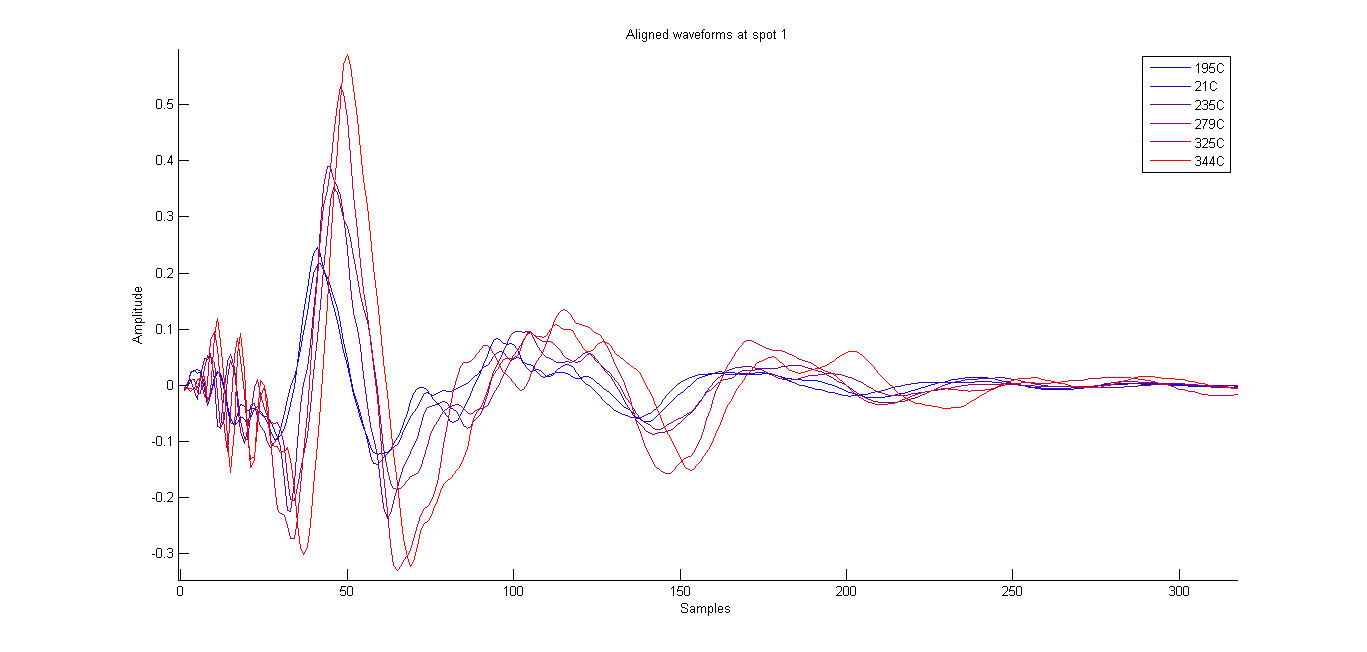
\includegraphics[width=150mm]{shiftOverTemperature.png}
\caption{6 different mean templates trained a 6 different temperatures on the same spot. Sampled at 44.1 kHz and aligned.}\label{fig:shiftOverTemperature}
\end{figure}
It appears that temperature has a dramatic effect on the mean template and therefore it seems questionable whether or not the previously described \gls{ml} and \gls{map} method would be able to cope with this level of variation. Pulse variability has also been detected when users hold the devices in different ways, have the device on a surface and tap with nails or different styluses. The \gls{pca} type method is an attempt at singling out significant components of the pulse that relate to the tapping position rather than the other factors mentioned above, and to record the variability within the significant components.

\begin{figure}[!]
\centering
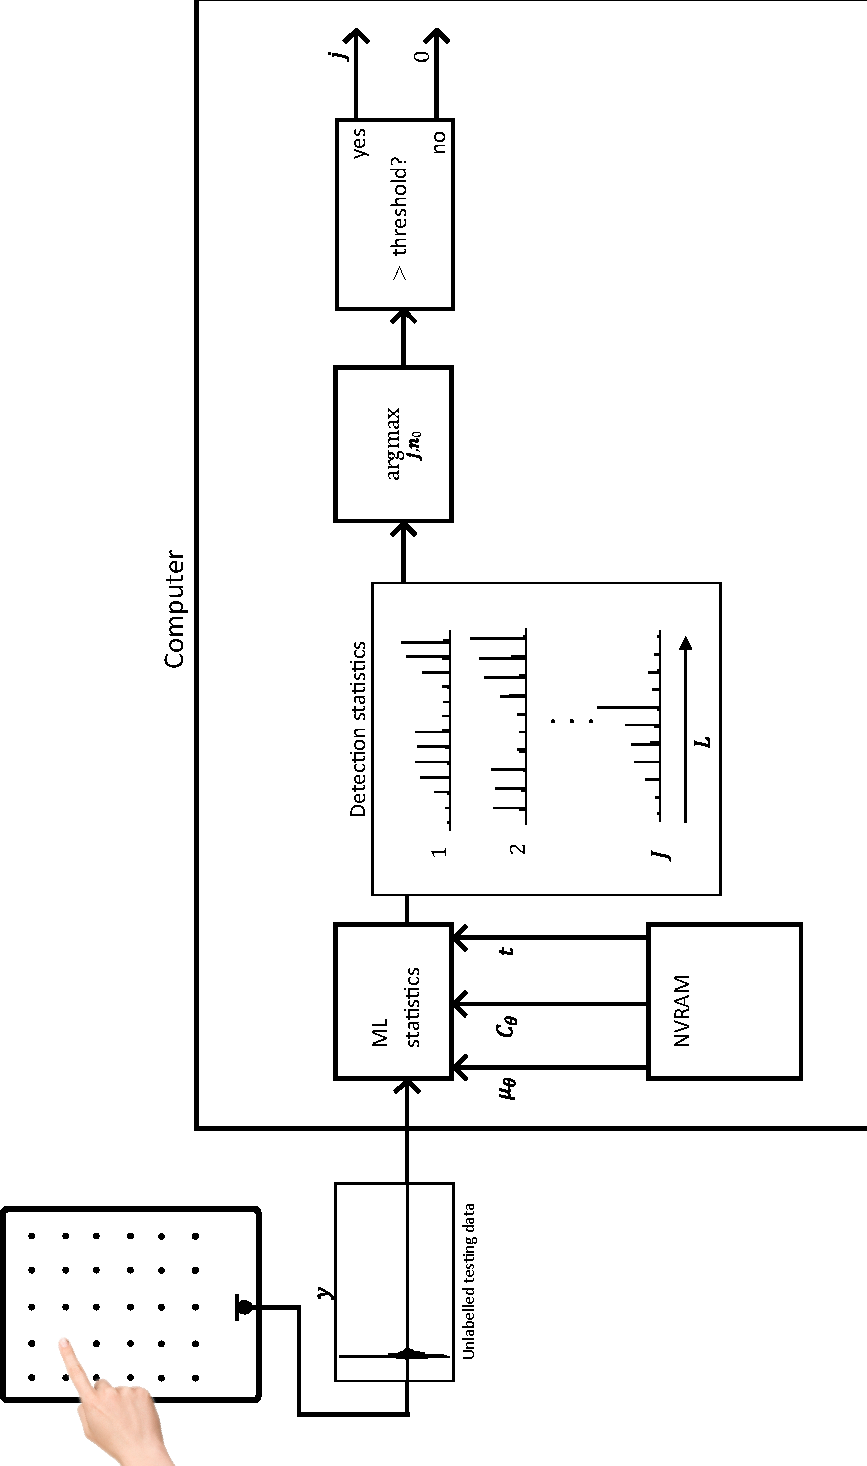
\includegraphics[width=360px]{testingSystemPlot.pdf}
\caption{Block diagram of detection/use stage of algorithm.}\label{fig:testingSystemPlot}
\end{figure}

Figure~\ref{fig:testingSystemPlot} shows a block diagram of the implementation of the use/testing stage of the algorithm. The diagram shows how a tap $y$ incident on the tapping device is picked up by the microphone on the device and transmitted to a computer. Within the computer the algorithm calculates the statistics, as outlined below, utilising data from the training stage of the algorithm. The statistics of the signal are then evaluated and the most probable class or spot is displayed to the user unless the models do not yield a sufficiently high probability, as determined by a threshold, in which case no tap will be registered.

\subsection{Model and theory}
A standard linear instantaneous model is considered where\linebreak[0] observations \linebreak[2]$y = [y_0, \ldots , y_{N-1}]^T $ are modeled as a noisy linear combination:

\begin{equation}\label{eq:mod1}
y = \sum_{i=1}^{I} \theta_i^j t_i^j(n_0) + v,
\end{equation}

where $\theta_i^j$ is the amplitude of the $j$th spot and $i$th component. $t_i^j(n_0)$ is the $j$th template, $j \in \{1, \ldots ,J\}$, for $I$ independent components where the templates are $N \times 1$ principal component vectors derived from a \gls{pca} of training data, as explained in more detail in section~\ref{sec:APRtraining}.

In this section the model has been assumed to be of zero mean $\mu^j(n_0) =0$ although this assumption could easily be avoided by adding the mean to the model as a variable to be estimated. Take $\theta_i^j$ to be a random variable, $\Theta^j = [\theta_1^j,\ldots,\theta_I^j]^T$, describing the scale of each template component $i$ where

\begin{equation}\label{eq:theta}
\Theta^j \sim \mathcal{N}(\mu_{\Theta}^j,C_{\Theta}^j),
\end{equation}

and Gaussian noise to model background interference:

\begin{equation}\label{eq:noisePCA}
v_n \stackrel{i.i.d.}{\sim} \mathcal{N}(0,\sigma^2).
\end{equation}

Considering this model in matrix notation:
\begin{equation}\label{eq:mod2PCA}
y = \textbf{t}\Theta + \textbf{v}.
\end{equation}

For simplicity the matrices $\textbf{t}^j(n_0)$ and $\Theta^j$ will from now on be referred to as simply $\textbf{t}$ and $\Theta$ respectively.
Bayes' theorem can now be used to evaluate the joint probability of $y$ and $\Theta$ as

\begin{equation}\label{eq:bayes1}
p(y,\Theta | j) = p(y|\Theta,j)p(\Theta | j).
\end{equation}

Since the goal is to evaluate the probability of each data reading $y$ given a particular position/model $j$, the dependency of $\Theta$ can be marginalized out,

\begin{eqnarray}\nonumber
p(y|j) &=& \int_\Theta p(y,\Theta|j) d\Theta \\
\label{eq:marg1} &=& \int_\Theta p(y|\Theta,j)p(\Theta|j) d\Theta.
\end{eqnarray}

Given (\ref{eq:noisePCA}) and (\ref{eq:mod2PCA}), the probability $p(y|\Theta,j)$ can be expressed as:

\begin{equation}\label{eq:probybeta}
p(y|\Theta,j) = \mathcal{N}_y(\textbf{t}\Theta,\sigma^2\textbf{I}),
\end{equation}
where $\textbf{I}$ is the identity matrix.
Now (\ref{eq:marg1}) can be written as:

\begin{equation}\label{eq:marg2}
p(y|j) = \int_\Theta \mathcal{N}_y(\textbf{t}\Theta,\sigma^2 \textbf{I})\times\mathcal{N}_\Theta(\mu_\Theta,C_\Theta) d\Theta
\end{equation}

The product of two normal distributions is another normal distribution and since this resulting normal distribution is no longer normalised a normalising constant $z$ is added:

\begin{equation}\label{eq:prod1}
\mathcal{N}_y(\textbf{t}\Theta,\sigma^2 \textbf{I})\cdot\mathcal{N}_\Theta(\mu_\Theta,C_\Theta) = z \times \mathcal{N}_\Theta(\hat{\mu}_\Theta,\hat{C}_\Theta)
\end{equation}

Since:
\begin{equation}\label{eq:marg3}
\int_\Theta \mathcal{N}_\Theta(\hat{\mu}_\Theta,\hat{C}_\Theta) d\Theta = 1,
\end{equation}
we have:
\begin{equation}\label{eq:marg4}
p(y|j) = z \times \int_\Theta \mathcal{N}_\Theta(\hat{\mu}_\Theta,\hat{C}_\Theta) d\Theta = z.
\end{equation}

To evaluate $z$, the l.h.s. of equation (\ref{eq:prod1}) is expanded
{\setlength\arraycolsep{2pt}
\begin{eqnarray}
\label{eq:prod2} & & \mathcal{N}_y(\textbf{t}\Theta,\sigma^2 \textbf{I})\times\mathcal{N}_\Theta(\mu_\Theta,C_\Theta) = \\\nonumber
& & \qquad \frac{1}{(2\pi)^{\frac{N}{2}} |\sigma^2\textbf{I}|^{\frac{1}{2}}} \textrm{exp}\left[-\frac{1}{2}(y - \textbf{t}\Theta)^T(\sigma^2 \textbf{I})^{-1}(y - \textbf{t}\Theta)\right] \times {} \\\nonumber
& & \qquad \frac{1}{(2\pi)^{\frac{N}{2}}|C_\Theta|^{\frac{1}{2}}} \textrm{exp}\left[-\frac{1}{2}(\Theta - \mu_\Theta)^TC_\Theta^{-1}(\Theta - \mu_\Theta)\right] \\\nonumber
& & \quad= \frac{1}{(2\pi)^N |\sigma^2\textbf{I}|^{\frac{1}{2}} |C_\Theta|^{\frac{1}{2}}} \textrm{exp}\bigg[-\frac{\textbf{I}}{2\sigma^2}\left(y^Ty+\Theta^T\textbf{t}^T\textbf{t}\Theta - 2 \Theta^T\textbf{t}y\right) - {} \\\nonumber
& & \qquad \frac{1}{2C_\Theta} \left(\Theta^T\Theta + \mu_\Theta^T\mu_\Theta - 2 \Theta^T\mu_\Theta\right) \bigg] \\\nonumber
& & \quad = \frac{1}{(2\pi)^N |\sigma^2\textbf{I}|^{\frac{1}{2}} |C_\Theta|^{\frac{1}{2}}} \textrm{exp}\Bigg[-\frac{1}{2}\Bigg(\Theta^T\left(\frac{\textbf{t}^T\textbf{t}}{\sigma^2} + C_\Theta^{-1}\right)\Theta - 2 \Theta^T\left(\frac{\textbf{t}y}{\sigma^2} + \frac{\mu_\Theta}{C_\Theta}\right) + {}\\\nonumber
& & \qquad \mu_\Theta^TC_\Theta^{-1}\mu_\Theta + \frac{y^Ty}{\sigma^2}\Bigg)\Bigg].
\end{eqnarray}}
The r.h.s. of equation (\ref{eq:prod1}) is also expanded,

{\setlength\arraycolsep{2pt}
\begin{eqnarray}
\label{eq:prod3} & & z \times \mathcal{N}_\Theta(\hat{C}_\Theta,\hat{\mu}_\Theta) \\\nonumber
& & \quad = z\frac{1}{(2\pi)^{\frac{N}{2}} |\hat{C}_\Theta|^{\frac{1}{2}}} \textrm{exp}\left[-\frac{1}{2}\left(\Theta - \hat{\mu}_\Theta\right)^T\hat{C}_\Theta^{-1}\left(\Theta - \hat{\mu}_\Theta\right)\right] \\\nonumber
& & \quad = z\frac{1}{(2\pi)^{\frac{N}{2}} |\hat{C}_\Theta|^{\frac{1}{2}}} \textrm{exp}\left[-\frac{1}{2}\left(\Theta^T\hat{C}_\Theta^{-1}\Theta + \hat{\mu}_\Theta^T\hat{C}_\Theta^{-1}\hat{\mu}_\Theta - 2\Theta^T\hat{C}_\Theta^{-1}\hat{\mu}_\Theta\right)\right],
\end{eqnarray}}
and by inspection and comparison between equation (\ref{eq:prod2}) and (\ref{eq:prod3}) it is found that:

\begin{eqnarray}
\label{eq:prod4}
\hat{C}_\Theta &=& \left(\frac{\textbf{t}^T\textbf{t}}{\sigma^2} + C_\Theta^{-1}\right)^{-1} \qquad \textrm{and}\\\nonumber
\hat{\mu}_\Theta &=& \left(\frac{\textbf{t}^Ty}{\sigma^2} + \frac{\mu_\Theta}{C_\Theta}\right)\hat{C}_\Theta.
\end{eqnarray}

Equation (\ref{eq:prod2}) and (\ref{eq:prod3}) are equated and the normalizing constant $z$ is isolated.

{\setlength\arraycolsep{2pt}
\begin{eqnarray}\label{eq:z1}
z &=& \frac{(2\pi)^{\frac{N}{2}}\left|\hat{C}_\Theta\right|^{\frac{1}{2}} }{(2\pi)^n |\sigma^2\textbf{I}|^{\frac{1}{2}} |C_\Theta|^{\frac{1}{2}}} \times {}\\\nonumber
& &\frac{\textrm{exp}\Bigg[-\frac{1}{2}\Bigg(\Theta^T\left(\frac{\textbf{t}^T\textbf{t}}{\sigma^2} + C_\Theta^{-1}\right)\Theta - 2 \Theta^T\left(\frac{\textbf{t}y}{\sigma^2} + \frac{\mu_\Theta}{C_\Theta}\right) + \mu_\Theta^TC_\Theta^{-1}\mu_\Theta + \frac{y^Ty}{\sigma^2}\Bigg)\Bigg]}{\textrm{exp}\left[-\frac{1}{2}\left(\Theta^T\hat{C}_\Theta^{-1}\Theta - 2\Theta^T\hat{C}_\Theta^{-1}\hat{\mu}_\Theta + \hat{\mu}_\Theta^T\hat{C}_\Theta^{-1}\hat{\mu}_\Theta \right)\right]}.
\end{eqnarray}}
Substituting $\hat{C}_\Theta$ from equation~(\ref{eq:prod4}) and doing some simplification, gives:
{\setlength\arraycolsep{2pt}
\begin{eqnarray}\label{eq:z2}
z &=& \frac{\left|\frac{\textbf{t}^T\textbf{t}}{\sigma^2} + C_\Theta^{-1}\right|^{-\frac{1}{2}}}{(2\pi)^{\frac{n}{2}} |\sigma^2\textbf{I}|^{\frac{1}{2}} |C_\Theta|^{\frac{1}{2}}} \times {}\\\nonumber
& &\frac{\textrm{exp}\Bigg[-\frac{1}{2}\Bigg(\Theta^T\left(\frac{\textbf{t}^T\textbf{t}}{\sigma^2} + C_\Theta^{-1}\right)\Theta - 2 \Theta^T\left(\frac{\textbf{t}y}{\sigma^2} + \frac{\mu_\Theta}{C_\Theta}\right) +  \mu_\Theta^TC_\Theta^{-1}\mu_\Theta + \frac{y^Ty}{\sigma^2}\Bigg)\Bigg]}{\textrm{exp}\left[-\frac{1}{2}\left(\Theta^T \left(\frac{\textbf{t}^T\textbf{t}}{\sigma^2} + C_\Theta^{-1}\right)\Theta  - 2\Theta^T\left(\frac{\textbf{t}^T\textbf{t}}{\sigma^2} + C_\Theta^{-1}\right)\hat{\mu}_\Theta  + \hat{\mu}_\Theta^T\left(\frac{\textbf{t}^T\textbf{t}}{\sigma^2} + C_\Theta^{-1}\right)\hat{\mu}_\Theta \right)\right]}
\end{eqnarray}}
Substituting $\hat{\mu}_\Theta$ from equation~(\ref{eq:prod4}) and doing some simplification, gives:
{\setlength\arraycolsep{2pt}
\begin{eqnarray}\label{eq:z25}
z &=& \frac{1}{(2\pi)^{\frac{n}{2}} |\textbf{t}^T\textbf{t}+\sigma^2C_\Theta^{-1}|^{\frac{1}{2}} |C_\Theta|^{\frac{1}{2}}} \times {}\\\nonumber
& &\frac{\textrm{exp}\Bigg[-\frac{1}{2}\Bigg(- 2 \Theta^T\left(\frac{\textbf{t}y}{\sigma^2} + \frac{\mu_\Theta}{C_\Theta}\right) +  \mu_\Theta^TC_\Theta^{-1}\mu_\Theta + \frac{y^Ty}{\sigma^2}\Bigg)\Bigg]}{\textrm{exp}\left[-\frac{1}{2}\left(- 2\Theta^T\left(\frac{\textbf{t}^Ty}{\sigma^2} + \frac{\mu_\Theta}{C_\Theta}\right)  + \left(\left(\frac{\textbf{t}^T\textbf{t}}{\sigma^2} + C_\Theta^{-1}\right)^T\right)^{-1}\left(\frac{\textbf{t}^Ty}{\sigma^2} + \frac{\mu_\Theta}{C_\Theta}\right)^T\left(\frac{\textbf{t}^Ty}{\sigma^2} + \frac{\mu_\Theta}{C_\Theta}\right) \right)\right]}\\\nonumber{}\\\nonumber
&=& \frac{1}{(2\pi)^{\frac{n}{2}} |\Phi|^{\frac{1}{2}} |C_\Theta|^{\frac{1}{2}}}\times \frac{\textrm{exp}\left[-\frac{1}{2\sigma^2}\left(\sigma^2\mu_\Theta^TC_\Theta^{-1}\mu_\Theta + y^Ty\right)\right]}{\textrm{exp}\left[-\frac{1}{2\sigma^2}\left(\left(\Phi^T\right)^{-1}\Lambda^T\Lambda \right)\right]}\\\nonumber{}\\\nonumber
&=& \frac{1}{(2\pi)^{\frac{n}{2}} |\Phi|^{\frac{1}{2}}|C_\Theta|^{\frac{1}{2}}} \textrm{exp}\left[-\frac{1}{2\sigma^2}\left(\sigma^2\mu_\Theta^TC_\Theta^{-1}\mu_\Theta + y^Ty- \left(\Phi^T\right)^{-1}\Lambda^T\Lambda\right)\right],
\end{eqnarray}}
where:
\begin{eqnarray}
\label{eq:z3}
\Phi &=& \textbf{t}^T\textbf{t} + \sigma^2C_\Theta^{-1} \qquad \textrm{and}\\\nonumber
\Lambda &=& \textbf{t}^Ty + \sigma^2\mu_\Theta C_\Theta^{-1}.
\end{eqnarray}

As with the previous method, the log-likelihood is calculated

\begin{equation}\begin{split}\label{eq:loglikeli}
\log{p(y|j)} = &- \frac{n}{2}\log{2 \pi}- \frac{1}{2}\log{|\Phi|} - \frac{1}{2}\log{|C_\Theta|} \\
&- \frac{1}{2\sigma^2}\left(\sigma^2\mu_\Theta^TC_\Theta^{-1}\mu_\Theta + y^Ty- \left(\Phi^T\right)^{-1}\Lambda^T\Lambda\right),
\end{split}\end{equation}

and maximised over the $J$ different templates, similar to equation~(\ref{eq:MLdefinition}).

\section{Amplitude variable PCA model}\label{sec:KamplitudeModel}

To account for linear scaling of the signal $x$, a modified \gls{pca} model is constructed. While the $\theta$ parameter of the \gls{pca} approach assumes that each pulse is a combination of a set of components observed during training, the strength of impact on the surface will translate into an increased amplitude of the pulse waveform. The aim of the variable amplitude model is to separate out this scale as a random variable $K$. In the basic \gls{pca} model the pulse amplitudes were represented in the $\theta$ parameter and in this model the amplitudes will be represented as $K$ and then subsequently normalized.

Recalling the standard multi-variate \gls{pca} based approach with mean $\mu$ zero (see equation \ref{eq:mod1}), we had

\begin{equation}\label{eq:K_PCAmodel}
y = \sum^I_{i=1} \theta^j_i t^j_i(n_0) + v.
\end{equation}

For $K$ a vector of scalar amplitudes for the combined instantaneous linear combination, we can write,

\begin{equation}\label{eq:Kmodel}
y = K^j \sum^I_{i=1} \theta^j_i t^j_i(n_0) + v.
\end{equation}

Here $K^j$ is the scaling amplitude for the $j$th template.

Considering previously equation~\ref{eq:probybeta}, we can now model the signal $y$ as:

\begin{equation}\label{eq:GP2}
    p(y|j,n_0,K) = \mathcal{N}_y(K^j \Theta^j \textbf{t}^j(n_0) , \sigma^2),
\end{equation}

where $K_j$ is a random variable describing the linear scaling of the model.

In equation~\ref{eq:MLmargin} the continuous component scaling factor $\theta$ was marginalised out to give $p(y|j,n_0)$. In much the same way, the likelihood can be estimated by evaluation of the joint probability of the data $y$ given a discrete scaling $K$, template number $j$ and the time shift $n_0$, over $K$.

For $K$, $p(K)$ is now considered to be a discretely sampled distribution such that

\begin{equation}\label{eq:pkldefine}
Pr\left\{K = k_l\right\} = p_{K,l},
\end{equation}

for the $l = 1:L$ samples of $p(K)$.

The sampling of $p(K)$ can now be expressed as
\begin{equation}\label{eq:sampledK}
p(K|j) = \sum_{l=1}^L p^j_{K,l} \delta \left(K - k_l\right),
\end{equation}

and the signal $y$ can now be modeled as

\begin{eqnarray}\label{eq:MLmarginK}
p(y|j,n_0) &=& \int \sum_{l=1}^L p(y|j, n_0, K=k_l) p^j_{K,l} \delta \left(K - k_l\right) dK\\
&=& \sum_{l=1}^L p(y|j, n_0, K=k_l) p^j_{K,l}.
\end{eqnarray}

The distribution of $p(K|j)$ could be estimated as a discrete point-mass \linebreak[0](positive-valued) inverse-gamma distribution or simply sampled at a training stage for each class $j$. In this case $p(K|j)$ is assumed to be discrete and equation~\ref{eq:MLmarginK} is a finite sum of weighted Gaussian terms. In the continuous cases the integral could be computed using Monte Carlo integration approximated using discrete summation.

Proceeding with the steps from equation~\ref{eq:marg2} - \ref{eq:z25} (the full derivations are available in Appendix~\ref{ap:AppDeriv}, the log-likelihood is calculated

\begin{equation}\label{eq:loglikeliK}\begin{split}
\log{p(y|j,n_0,\theta,K)} = &- \frac{n}{2}\log{2 \pi}- \frac{1}{2}\log{|\Phi|} - \frac{1}{2}\log{|C_\Theta|} \\
& -\frac{1}{2\sigma^2}\left(\sigma^2\mu_\Theta^TC_\Theta^{-1}\mu_\Theta + y^Ty- \left(\Phi^T\right)^{-1}\Lambda^T\Lambda\right),
\end{split}\end{equation}

where
\begin{eqnarray}
\label{eq:z3K}
\Phi &=& K^2 \textbf{t}^T\textbf{t} + \sigma^2C_\Theta^{-1} \qquad \textrm{and}\\\nonumber
\Lambda &=& K \textbf{t}^Ty + \sigma^2\mu_\Theta C_\Theta^{-1}.
\end{eqnarray}

\section{Training}\label{sec:APRtraining}
In order to be able to deploy the above mentioned models, the templates needed in the models must be created. The term ``training'' is here used to refer to the process of creating the matrices $t$ and $t^j_i(n_0)$ containing the $J$ models and $I$ components, the covariance matrix $C^j_\Theta$ and the mean $\mu^j_\Theta$.

To train a template for a spot, a large quantity of tapping data is recorded from the device and stored. This tapping data is labeled, that is, the spot which was tapped to create the tapping pulse is known and the tapping data is divided into separate streams depending on this label. To pick out the individual taps from the audio stream, a representative tap is manually chosen from each stream and used as the coefficients in a correlation detector, the results of which are used to determine the alignment of the individual taps in the audio stream. A correlation detector, in this context, refers to a matched filter with a sample representative pulse used as the filter parameters with the output thresholded in some way. Figure~\ref{fig:correlationDetect} shows a short audio stream of taps where the red dots indicate detected taps.

\begin{figure}[!]
\centering
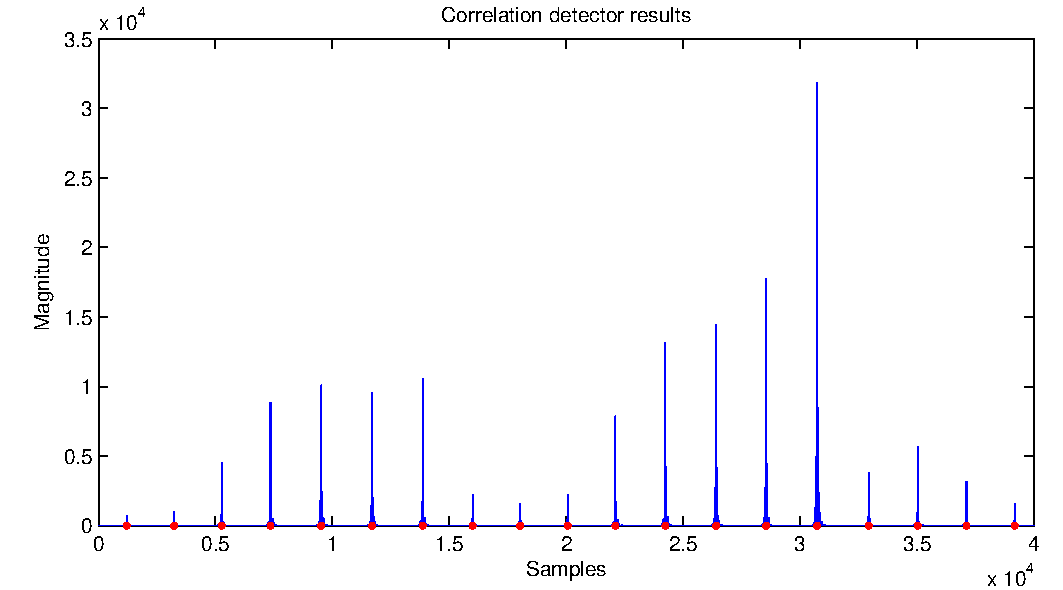
\includegraphics[width=150mm]{correlationDetect.pdf}
\caption{Output of correlation detection code. The plot shows the output of the matched filter using a manually picked pulse as a template and the red dots indicate detected taps via a simple thresholding.}\label{fig:correlationDetect}
\end{figure}

With all the taps in the audio stream detected it is now possible to align them for further processing.

\begin{figure}[!]
\centering
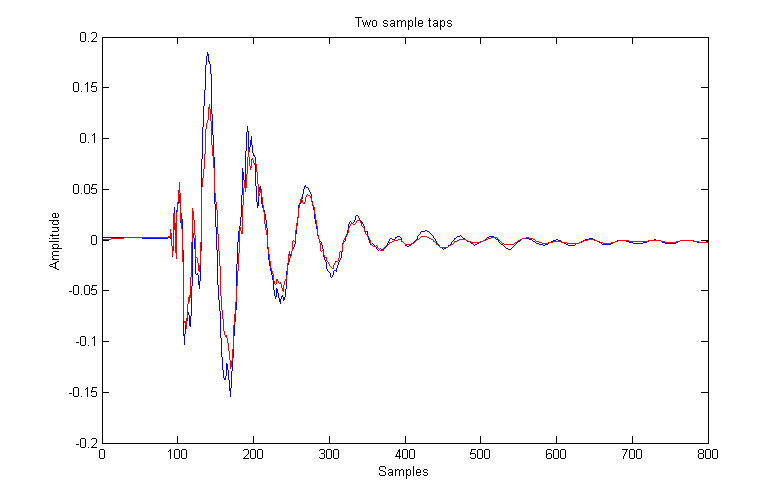
\includegraphics[width=110mm]{twoSampleTaps.png}
\caption{Two taps recorded at the same spot immediately after each other. Sampled at 44.1 kHz.}\label{fig:twoSampleTaps}
\end{figure}

Figure~\ref{fig:twoSampleTaps} shows a modest example of the variability that exists when tapping an object in seemingly the exact same manner. This variability is partly due to noise but bigger variations in the waveform are more likely caused by minute variations in tapping position, intensity and method. In an attempt to obtain a 1 dimensional model that represents a diverse selection of taps at the same spot for the \gls{ml} and \gls{map} method, the model is constructed as a mean of an ensemble of taps at this position. The mean template is manually trimmed to minimise data size and avoid excessive data that carries no useful information about the template. Figure~\ref{fig:alignedAndMean} shows a diverse set of aligned taps at a single point in blue and the corresponding mean in red.

\begin{figure}[!]
\centering
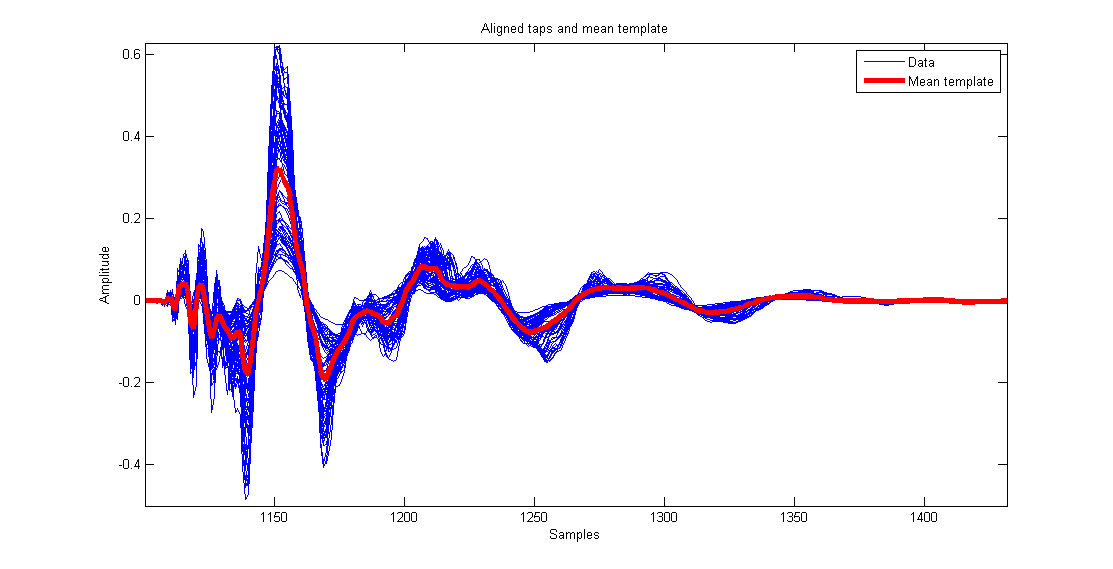
\includegraphics[width=150mm]{alignedAndMean.png}
\caption{Aligned taps with corresponding mean template superimposed on top. Sampled at 44.1 kHz.}\label{fig:alignedAndMean}
\end{figure}

Due to the nature of this algorithm it is essential that it can be executed rapidly and in real time. To accomplish a rapid execution, sub-calculations, independent of $y$, from equation (\ref{eq:MLloglikelihood}) have been pre-computed.

The \gls{pca} type method requires a different type of template. Here the template is derived via a \gls{pca} of the covariance matrix derived from the aligned tapping data as described above.

First the mean and the covariance matrices for each spot $j$ are calculated:

\begin{eqnarray}\nonumber
\mu^j &=& \frac{1}{N^j} \sum_k x^j_k \\\label{eq:PCAcovariance}
C^j &=& \frac{1}{N^j}\sum_k \left(x^j_k - \mu^j\right)\left(x^j_k - \mu^j\right)^T,
\end{eqnarray}
where $x^j_k$ is the $k$th segment of the tapping stream containing a tap on the $j$th spot and $N^j$ is the sample length of the $j$th template. The eigenvalues and the eigenvectors of the covariance matrices $C^j$ are then computed, and the required number of components $q$ (eigenvectors) are chosen based on the corresponding descending values of the eigenvalue. Figure~\ref{fig:eigenvalues} shows an example of a descending order of eigenvalues from an eigenvalue decomposition of the covariance matrix $C^j$.

\begin{figure}[!]
\centering
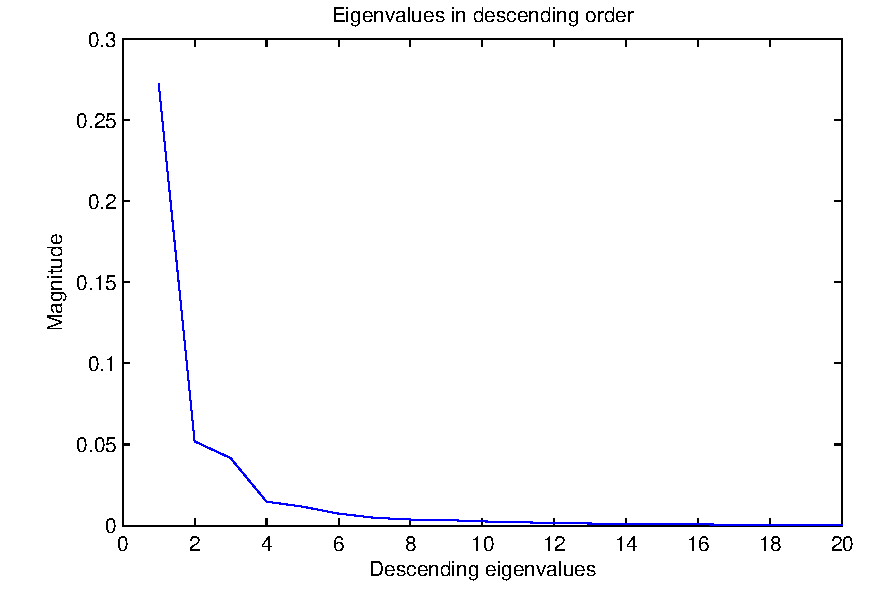
\includegraphics[width=120mm]{eigenvalues.pdf}
\caption{Descending eigenvalues from a eigenvalue decomposition of a covariance matrix $C^j$.}\label{fig:eigenvalues}
\end{figure}

As with the previous method, it is also possible to allocate sub-calculations independent of $y$ from equation~(\ref{eq:z2}) to the training stage to avoid heavy calculations during runtime. In addition, $\mu_\Theta$ is also defined during the training stage.

Figure~\ref{fig:trainingsytemRotate} shows a block diagram of the implementation of the training algorithm. The training data $x^j$ is acquired by the user tapping multiple times on a specific spot $j$. The $N$ taps in this data stream $x^j$ are then detected and aligned with each other as an ensemble in a matrix. Figure~\ref{fig:trainingsytemRotate} shows this as $\textbf{x}^j =  [ x_1^j, x_2^j, \ldots , x_N^j ] $ and as the $N$ taps superimposed on each other in the little plot. From the ensemble the mean $\mu^j$ and the covariance matrix $C^j$ are computed, and from the covariance matrix $C^j$ the eigenvalues and eigenvectors are derived. The $q$ largest eigenvalues are selected and the corresponding eigenvectors are stored as the templates $t^j = [\alpha^j_1,\alpha^j_2,\ldots,\alpha^j_q] $ while the eigenvalues are stored as $C_\Theta^j = diag\{\lambda_1^j,\lambda_2^j,\ldots,\lambda_q^j \}$.

\begin{figure}[!]
\centering
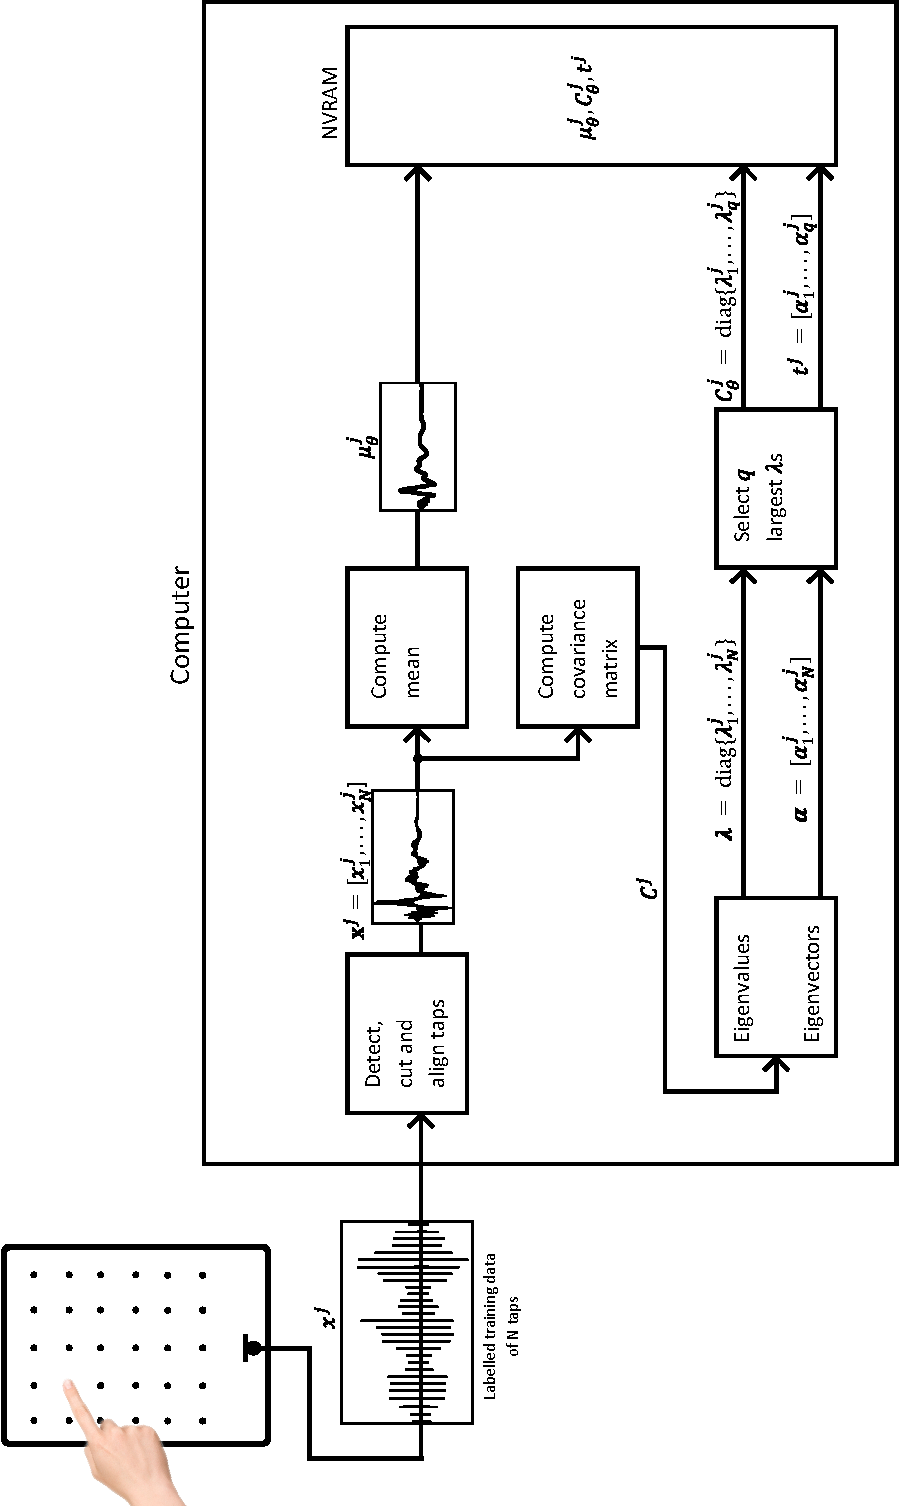
\includegraphics[width=360px]{trainingsytemRotate.pdf}
\caption{Block diagram of training stage of algorithm.}\label{fig:trainingsytemRotate}
\end{figure}

\subsection{Amplitude variable PCA model}

In addition to the parameters required for the standard \gls{pca} model, the amplitude variable model requires information about the scaling parameter $K$. Here we propose to sample $K^j = [K^j_{l=1}, \ldots , K^j_{l=L}]$, from the aligned training pulses recorded. Figure~\ref{fig:amplitudeProbMass.pdf} shows an example of the sampled probability mass functions used for three different models $j$. The sampling is done from a kernel smoothed distribution of amplitudes of the ensemble of pulses recorded. While $K^j$ is a discrete scaling vector for each model $j$ Figure~\ref{fig:amplitudeProbMass.pdf} shows continuous smoothed functions to better illustrate some of the variety in the models and to be able to plot them together. Each scaling vector $K^j$ comprises $L=100$ scales.

\begin{figure}
\centering
  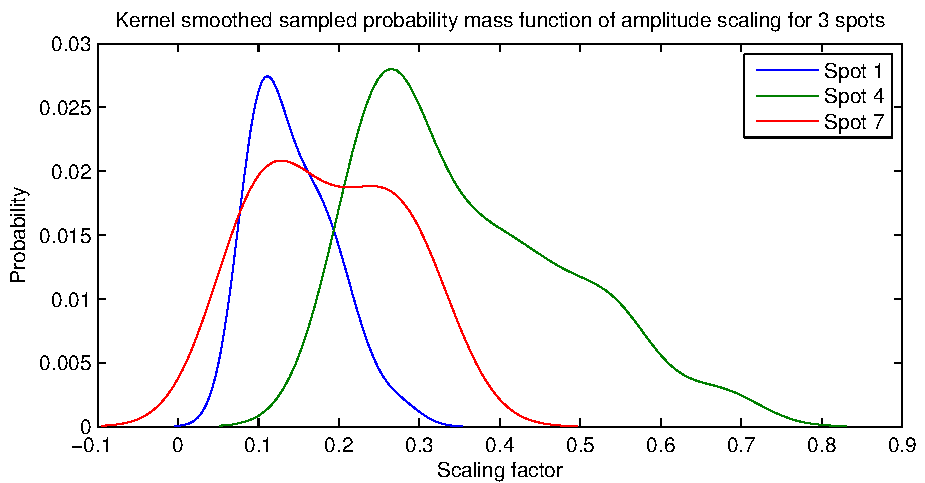
\includegraphics[width=110mm]{amplitudeProbMass.pdf}\\
  \caption{Kernel smoothed discrete probability mass function of 3 different spots for microphone 1.}\label{fig:amplitudeProbMass.pdf}
\end{figure}

\subsection{Sparse training extension}\label{sec:APRspareTraining}
The methods outlined above require labeled training data for each model in the classifier. Since it is entirely manageable to obtain this data for low resolution implementation of the pulse recognition system, obtaining this data on a larger device with a greater resolution can become cumbersome and time consuming. This extension of the standard training method for the \gls{ml} and \gls{map} methods enables detection of points outside the training grid at a scalable resolution.

To achieve this extended resolution, the algorithm creates a linear interpolation between neighboring templates. The assumption is that the acoustic pulses vary relatively linearly between the two templates and hence it may be possible to estimate any template in between the two. Since the mobile phone, used for the previous implementation, undoubtedly is a very complicated vibrational system it was hypothesised that the solid wooden board might provide a more predictable vibrational system and hence a better implementation platform for the interpolation algorithm.

For a number of tapping spots evenly distributed on a line, the interpolated template $t$ at position $x$ along the line on the board can be interpolated by

\begin{equation}\label{eq:interp}
t = t_0 + \left(x - x_0\right) \frac{t_{1} - t^j}{x_1 - x_0},
\end{equation}

where $t_0$ and $t_1$ are the templates at the positions $x_0$ and $x_1$ respectively and \linebreak[0]$x_0 < x < x_1$.

An example of a section of the waveforms resulting from this interpolation can be seen in Figure~\ref{fig:InterpData}. Here the thick lines represent the templates computed from data while the thin lines are interpolated templates. The linearly varying color, between red and black of the thin lines, shows the relative distance of the template position $x$ in this example.

\begin{figure}[!]
\centering
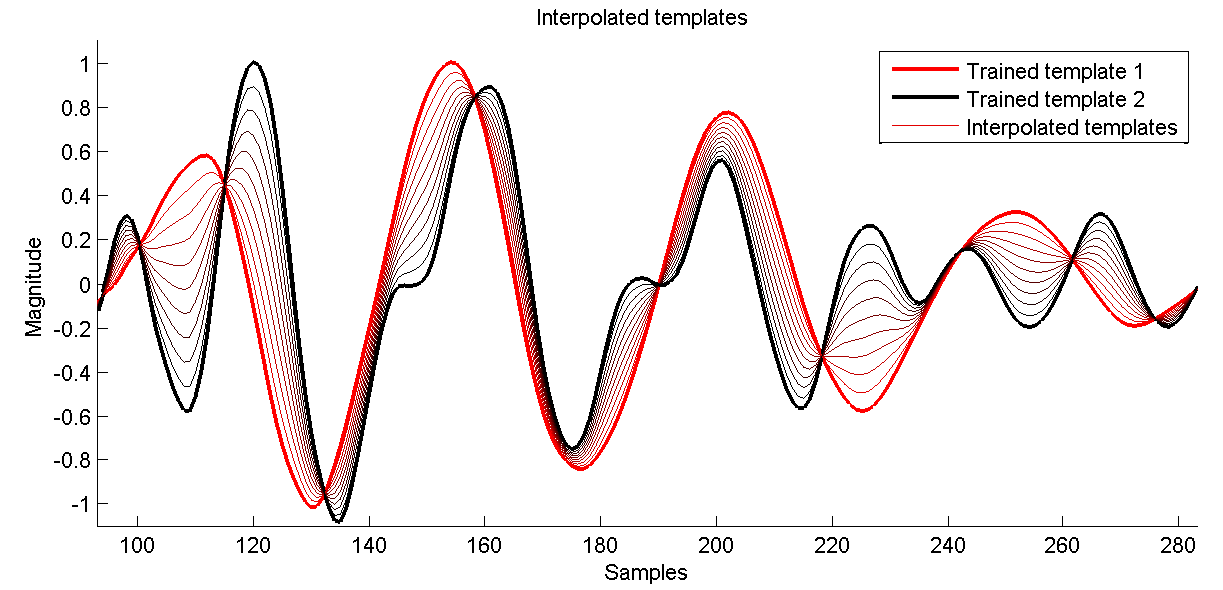
\includegraphics[width=360px]{InterpData.pdf}
\caption{Example of section of a interpolated waveforms using linear interpolation.}\label{fig:InterpData}
\end{figure}

To achieve a full 2D grid of interpolated templates amongst templates derived from data, requires a second round of interpolation in the second dimension for each column.

While the assumption of linearly changing pulses might be valid, it is still necessary to align the neighboring templates accurately. Aligning taps accurately has proven difficult with the correlation method due to the change in the pulses over the surface of the board. To provide a more accurate alignment method a second microphone was attached to the stylus while tapping to provide a consistent reference tap. The idea was that this consistent tap should provide exact alignment between all the taps. Figure~\ref{fig:templatesAligned} shows the result of this alignment.

\begin{figure}[!]
\centering
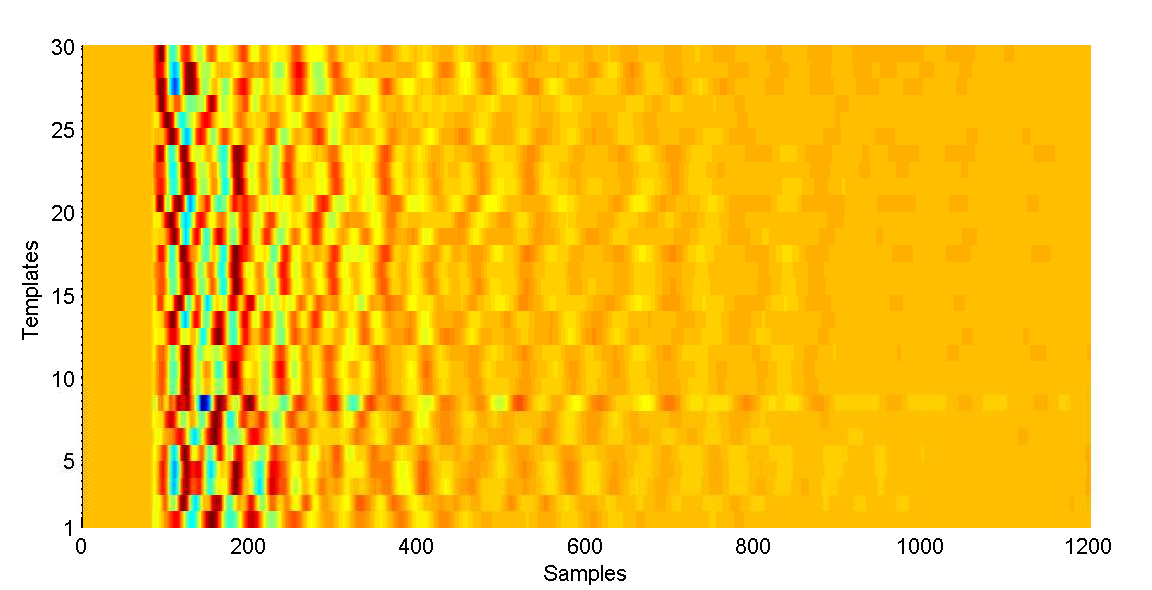
\includegraphics[width=380px]{templatesAligned.pdf}
\caption{30 templates from wooden board aligned. Seen from above.}\label{fig:templatesAligned}
\end{figure}

The benefit of a representation like Figure~\ref{fig:templatesAligned} is that it shows the wooden board is laid out in a grid of 6 by 5 spots, spot numbering starting in top left corner and following reading direction, which allows for assessment of alignment row by row.

The standard 6 by 5 spot resolution on the wooden board can be expanded to 51 by 41 spots simply by interpolating 9 templates between each trained spot row-wise and then doing the same for all 41 columns. The running of the detection algorithm will proceed as before although at a substantially slower rate.

\section{Methods}
\subsection{Performance and comparison of ML, MAP and PCA methods}
To test the algorithms, two sets of data are needed; a training set $D^1$ and a testing set $D^2$. The training set is used in the training stage of the algorithm, as mentioned above, and the testing data is essentially the data that the algorithm attempts to model and classify. In an attempt to evaluate the algorithms' robustness to variations, two different sets of training and testing data were used. One set was recorded using a stylus to tap on the device, $D^1_S$ and $D^2_S$, and the second set was tapped using a finger nail, $D^1_N$ and $D^2_N$. Although it might be informative to use the same data for the training and testing stage, in this test the two sets were independently recorded, in identical conditions, which means that there in total are 4 data sets $D^1_S$, $D^2_S$, $D^1_N$ and $D^2_N$, which will be used to test the algorithms in various combinations giving a picture of the performance of the algorithms. Figure~\ref{fig:tapSN} shows the tapping of the surface of the device with a stylus and with a fingernail.

\label{corrections:DSNmethod}All data was recorded in a quiet recording environment with the device held in the left hand while tapping with the right hand by a single user. A plastic stylus, as depicted in Figure~\ref{fig:tapSN}, was used for the stylus data, although it was noted that other hard plastic devices could produce similar pulses in the device. Each location was tapped continuously for exactly 20 seconds at the same rate producing a near identical number of taps per spot. The device was struck with a varying and random amount of force to simulate a user's varying usage characteristics. Although the specific spot on the device was the targeted strike point it is difficult to quantify the exact variability of the striking point overall testing and training. Since no particular effort was made to be more or less precise in the training or testing sets it is believed that any variability in precision would be negligible.

\begin{figure}[!]
\centering
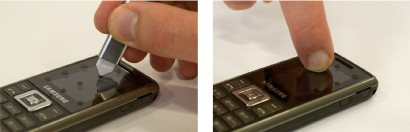
\includegraphics[width=410 px]{tapSN.png}
\caption{To the left is an example of a tap with the stylus and to the right a tap with a fingernail.}\label{fig:tapSN}
\end{figure}

\begin{figure}[!]
\centering
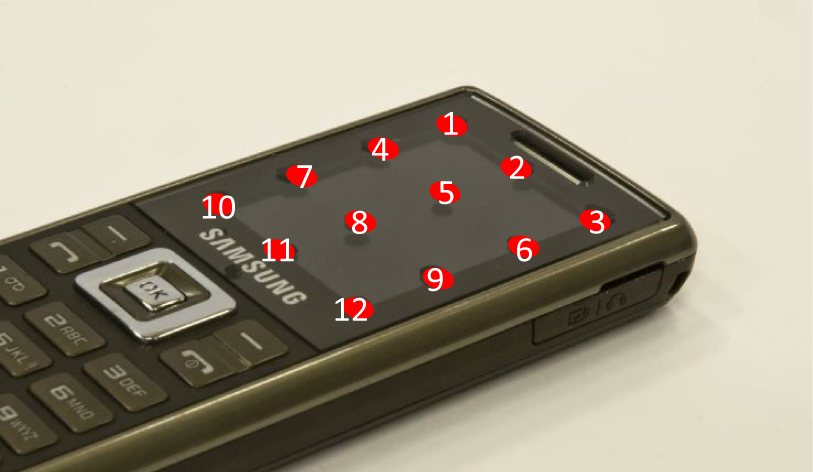
\includegraphics[width=300 px]{phoneDisplayNum.png}
\caption{Phone with spot location and numbers.}\label{fig:phoneDisplayNum}
\end{figure}

Figure~\ref{fig:phoneDisplayNum} shows the 12 spots and their location on the front of the phone used in this chapter.

Each set of training data contains approximately 70 taps\label{corrections:DSNcount} at each spot on the device totalling approximately $70 \times 12 = 840$ taps tapped with varying force. To estimate the performance of the algorithm given certain criteria there are 3 outcomes of a test. The tap may be correctly classified, misclassified (classified as any of the 11 other spots) or it may avoid detection entirely and hence be classified as a missed detection $j=0$. The ratio of these 3 outcomes may vary with a large number of parameters within the algorithm such as various thresholds for detection or classification, template length, filtering or number of principal components used under training, so the performance of the algorithm will always be presented in relation to a varying parameter. It is worth noting that all data used in the production of these results have been high-pass filtered with a cut-off frequency of 1102.5 Hz (0.05 times the Nyquist frequency was found to be an effective cut-off frequency\label{corrections:cut-off}). The effect of this filtering has not exhaustively been investigated, but provides a ``cleaner'' signal, visually as well as removing background noise, and does not appear to harm the performance. Figure~\ref{fig:filterCompareSpectrogram} shows an example of the filtering on short pulse sequence. On the left the unfiltered signal can be seen while the right shows the signal filtered signal spectrogram. The effect of filtering on the visible spectrogram is clearly minimal.

\begin{figure}[!]
\centering
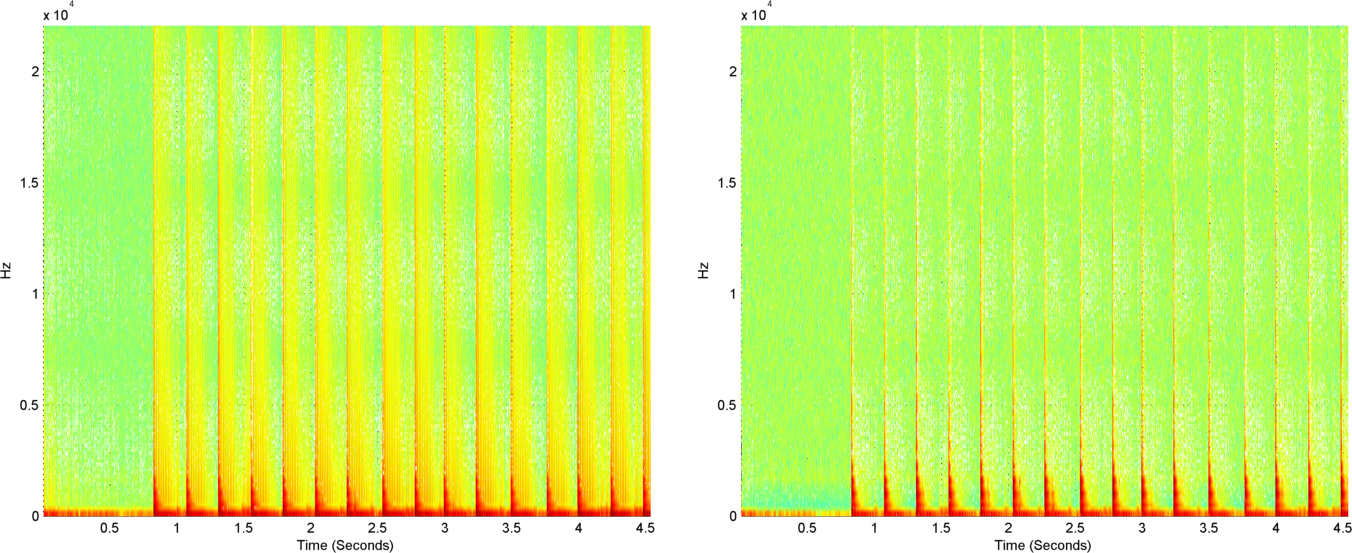
\includegraphics[width=410 px]{filterCompareSpectrogram.png}
\caption{Left, original pulse sequence. Right, pulse sequence high-pass filtered at 1102.5 Hz (cut-off), FIR 50 taps.}\label{fig:filterCompareSpectrogram}
\end{figure}


\begin{figure}[!]
\centering
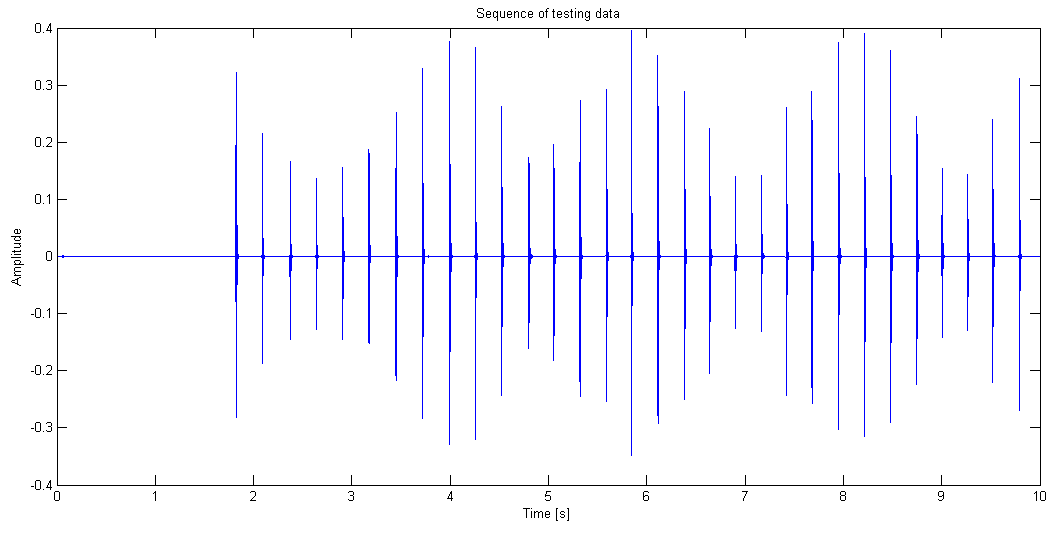
\includegraphics[width=410 px]{dataSequence.png}
\caption{Example of testing data variability.}\label{fig:dataSequence}
\end{figure}

Figure~\ref{fig:dataSequence} shows an example of a testing data sequence. While recording the testing, as well as training, data great care is taken to vary a range of parameters of the tap. From Figure~\ref{fig:dataSequence} is the clearly seen that the tapping force is varied resulting in a varying pulse amplitude, but the strike angle is also varied to replicate natural variability. The exact tapping location will also vary due to the manual nature of the data collection.


As well as evaluating the classification performance of some of the algorithms presented above, the effect of varying various parameters of the models, such as component number and template length, is also explored.

\subsection{Amplitude variable model}
The amplitude variable \gls{pca}, henceforth known as \gls{k-pca}, model presented in section~\ref{sec:KamplitudeModel} will be compared to the standard \gls{pca}  approach from section~\ref{sec:APRpca} to gauge if there is an advantage gained by adding the additional $K$ scaling factor to the model.

The data used for this comparison will be the same as that outlined in section~\ref{sec:MultiAPRMethod} and comprises a 9 spot model trained on a wooden board. The two methods will be compared based on three different data channels/microphones each at different locations and in two different environments. Figure~\ref{fig:NoisyMicSignalsCompare} shows an example of the audio waveform for the two different environments, for two of the three channels. A total of 79 audio segments from the relatively noiseless environment and 48 from the noisy environment were used. Each segment contained a single pulse from a random spot on the surface. Details of the system can be found in appendix~\ref{ap:MultiAPRsystem}.

The templates used in the comparison were identical in all other aspects than the parameters $K$ and $p(K)$. For the varying number of scale levels $L$ numbers were chosen so that $K$ and $p(K)$ could simply be decimated and $p(K)$ re-scaled.

For each method, and for each environment, an average of the performance of the three channels/microphones is presented. The raw data for all channels can be found in appendix~\ref{ap:KPCAresults}. The \gls{k-pca} was tested with a variety of discrete scaling parameters $L$ from 1 to 100.

\section{Results}\label{sec:results}
\subsection{ML, MAP and PCA methods}
In this section the empirical evaluations of the methods mentioned above are presented.

Figure~\ref{fig:PCAperform} shows the performance of the \gls{pca} type algorithm using the training data $D^1_S$ and the testing data $D^2_S$. The figure gives an idea of how the performance changes with the changing number of components, $q$, used in the templates. Figure~\ref{fig:PCAperform} clearly shows that the rate of correct classification is beyond 90\% down to 2 components whereafter it drops off sharply to below 10 \%. It is noted that the performance drops to around 8\% which is exactly what would be expected by a random guess or the prior knowledge $p(j)= \frac{1}{J}$. A decrease in performance is detectable from 4 components and down, whereas the performance for 5 components and more appears constant.

\begin{figure}[!] %PCA components S-S
\centering
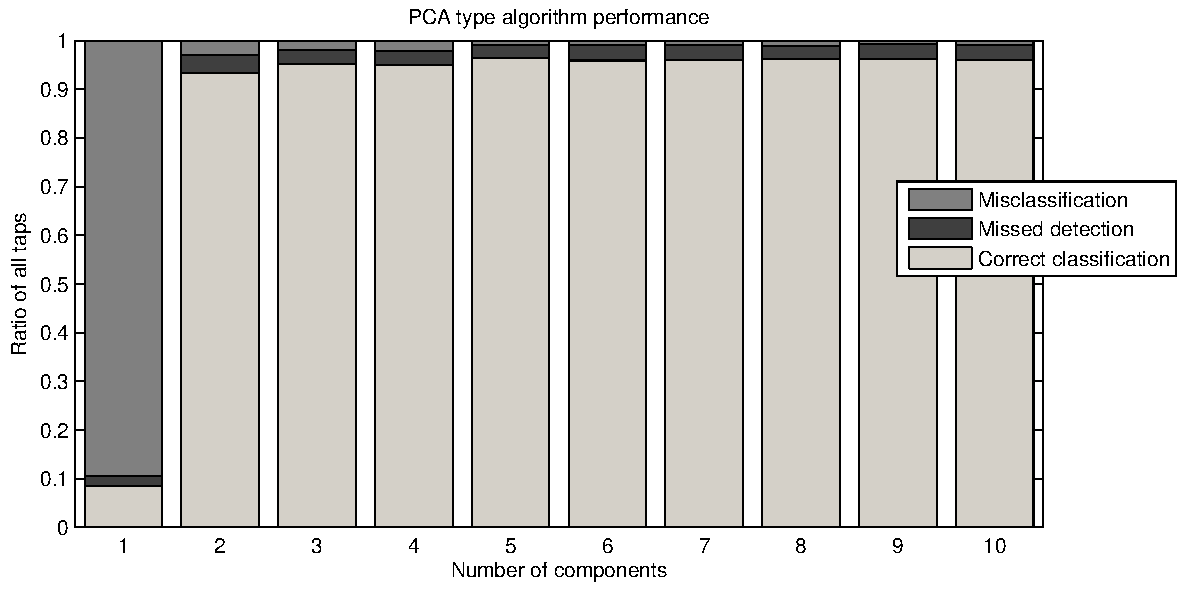
\includegraphics[width=150mm]{PCAperform.pdf}
\caption{Performance of the \gls{pca} type algorithm for different numbers of \gls{pca} components and with a template length $M=250$ samples. Training data: $D^1_S$, Testing data: $D^2_S$.}\label{fig:PCAperform}
\end{figure}

In Figure~\ref{fig:PCAperformLength} the relation between performance and template length $M$ can be seen with a test conducted with the same data as the previous test. The performance of the algorithm appears unaffected by $M$ at template lengths above 170 samples although for $M<170$ the performance decreases dramatically and as with Figure~\ref{fig:PCAperform} appears to settle around $p(j)$. The ratio between missed detections and misclassifications appear to vary greatly at low values for $M$ though it is currently not certain why this occurs. It is worth mentioning that this ratio is purely determined by a threshold in the algorithm and can be fine tuned for a desired outcome.

\begin{figure}[!] %PCA length S-S
\centering
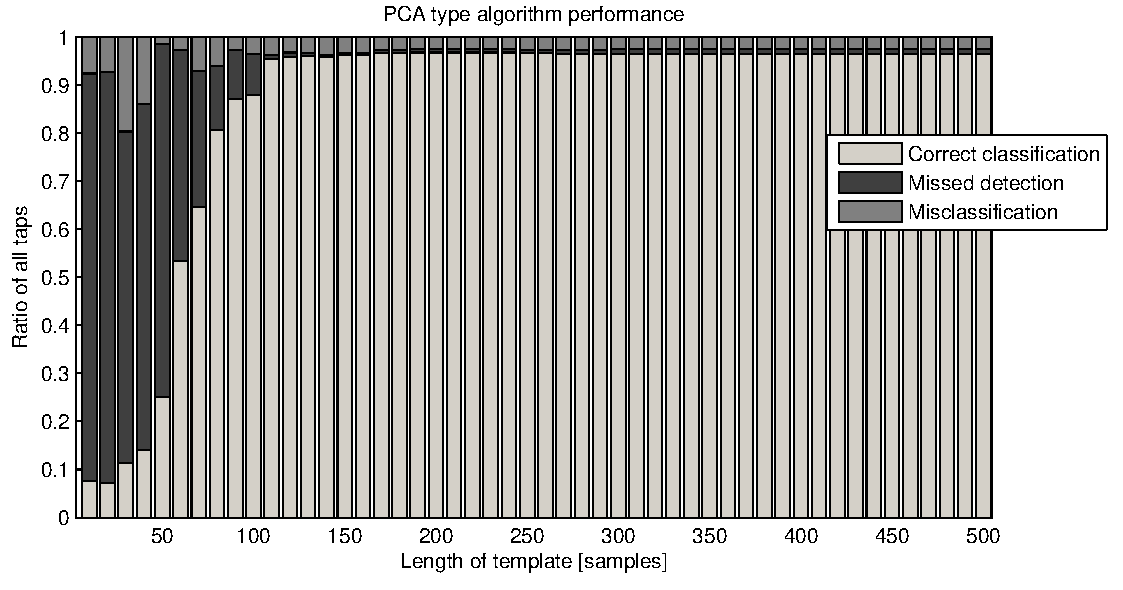
\includegraphics[width=150mm]{PCAperformLength.pdf}
\caption{Performance of the \gls{pca} type algorithm for different values of template length $M$ for components $q=5$. Training data: $D^1_S$, Testing data: $D^2_S$,}\label{fig:PCAperformLength}
\end{figure}

Figure~\ref{fig:MLperform} shows the performance of the \gls{ml} based algorithm using training data $D^1_S$ and testing data $D^2_S$. This figure shows the effect of changing the template length $M$ on the detection performance. As in Figure~\ref{fig:PCAperformLength} the performance appears to peak and stay constant at $M>170$. With the \gls{pca} algorithm the performance appears to approach the prior probability of detection at $M<50$ which, in this case, is set as being uniform across the different spots $j$.

Another feature of Figure~\ref{fig:MLperform} is the ratio of various detection results. Whereas the \gls{pca} type algorithm replaced correct classifications with misclassifications when the number of components fell below 5, the \gls{ml} algorithm appears to miss the detection of the tap entirely. This difference in the two methods is caused by a difference in the threshold for a missed detection.


\begin{figure}[!] %ML length S-S
\centering
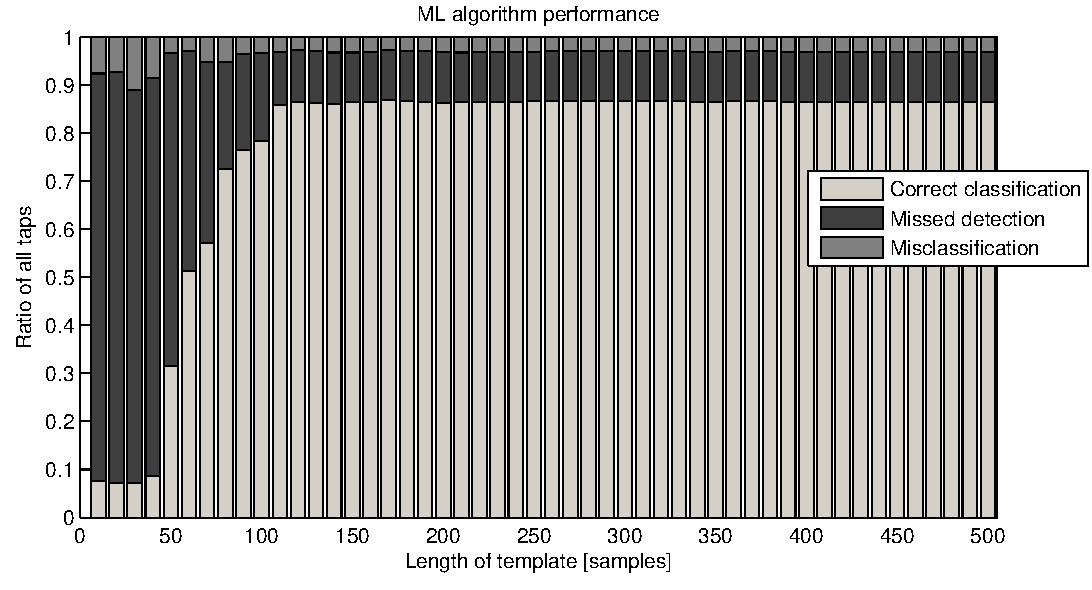
\includegraphics[width=150mm]{MLperform.pdf}
\caption{Performance of the \gls{ml} algorithm for different template sample lengths $M$. Training data: $D^1_S$, Testing data: $D^2_S$.}\label{fig:MLperform}
\end{figure}

For completeness Figure~\ref{fig:MAPperformLength} has been included to show the performance of the \gls{map} algorithm. The training and testing set up is identical to the previous evaluation of the \gls{ml} algorithm and the performance appears to be almost identical.

\begin{figure}[!] %MAP Length S-S
\centering
\includegraphics[width=150mm]{MAPperformLength.pdf}
\caption{Performance of the \gls{map} algorithm for different template sample lengths $M$. Training data: $D^1_S$, Testing data: $D^2_S$.}\label{fig:MAPperformLength}
\end{figure}

Figure~\ref{fig:PCAperformNail} shows the performance of the \gls{pca} type algorithm with $q$ again varying from 1 to 10, with training data $D^1_S$ and testing data $D^2_N$. In other words, the algorithm is tested by tapping using a finger nail but trained using only a stylus. This test is conducted to evaluate the \gls{pca} type algorithms ability to cope with testing data significantly different to the training data, and more specifically to evaluate the effect on the performance in relation to the number of components included, $q$. Figure~\ref{fig:PCAperformNail} shows a significantly reduced performance although the performance in relation to $q$ appears similar. For $q=1$ the performance still approaches $p(j)$.

\begin{figure}[!] %PCA components S-N
\centering
\includegraphics[width=150mm]{PCAperformNail.pdf}
\caption{Performance of the \gls{pca} type algorithm for different numbers of \gls{pca} components and with a template length of $M=250$ samples. Data used to evaluate performance was tapped using finger nails rather than the stylus used for training. Training data: $D^1_S$, Testing data: $D^2_N$.}\label{fig:PCAperformNail}
\end{figure}

The motivation for developing the \gls{pca} type algorithm was to be able to model data with a high degree of variability. Figure~\ref{fig:PCAperform_SN-SN} shows the performance of the \gls{pca} type algorithm in relation to changing $q$, with training being done with both the stylus $D^1_S$ and finger nail data $D^1_N$. By training on both sets it was hypothesised that the increased variability in the training data would be mirrored in the components, enabling the algorithm to cope with an equally increased degree of variability during the testing stage. To simulate the increased variability during the testing stage this test was conducted using stylus $D^2_S$ and finger nail $D^2_N$ data as well. Data presented in Figure~\ref{fig:PCAperform_SN-SN} suggests that this is the case.

\begin{figure}[!] %PCA components SN-SN
\centering
\includegraphics[width=150mm]{PCAperform_SN-SN.pdf}
\caption{Performance of the \gls{pca} type algorithm for different numbers of \gls{pca} components and with a template length $M=250$ samples. Training data: $D^1_S$ and $D^1_N$, Testing data: $D^2_S$ and $D^2_N$}\label{fig:PCAperform_SN-SN}
\end{figure}

Figure~\ref{fig:PCAMLMAPperform} gives an overview of the performance of the different algorithms with various data sets being used for testing and training. The specific data used for each test is noted on the figure itself. Please note that for all tests in Figure~\ref{fig:PCAMLMAPperform}, $M=250$ and $q=5$. These values were determined as sufficient in the previous tests detailed above.\

\begin{table}\begin{center}
\caption{Classification percentage correct results per channel for each algorithm with combined stylus and nail training and testing data.}
\label{tab:APRresultsPerChan}
\begin{tabular}{|c|c|c|c|c|c|c|c|c|c|c|c|c|}\hline
  & \multicolumn{12}{|c|}{Spot} \\
\hline
Method  & 1   & 2     & 3    & 4     & 5    & 6     & 7     & 8      & 9     & 10    & 11    & 12   \\ \hline
ML      & 86  & 100   & 90   & 98    & 99   & 100   & 43    & 100    & 100   & 39    & 100   & 76   \\
MAP     & 84  & 100   & 92   & 99    & 99   & 100   & 48    & 100    & 100   & 38    & 100   & 77   \\
PCA     & 99  & 100   & 93   & 100   & 99   & 100   & 99    & 100    & 100   & 100   & 100   & 100   \\ \hline
\end{tabular}\end{center}\end{table}

Table~\ref{tab:APRresultsPerChan} shows the percentage of correct detection, based on all detections, per spot for the three different methods. This data is generated from the templates trained on both the stylus and nail tapping data and tested on both data sets as well. It is seen that on spots 2, 5, 6, 8, 9 and 11 all methods perform similarly. On spots 1, 3, 4, 7, 10 and 12 the \gls{ml} and \gls{map} methods are performing worse than the \gls{pca}. Particularly spots 7 and 10 show a significantly reduced performance in the mixed training and testing scenarios. For more spot specific results with the \gls{pca} approach Tables~\ref{tab:multiAPRresultsPerChan} and \ref{tab:multiAPRresultsNoisePerChan} should be considered.

\begin{figure}[!] %PCA-ML-MAP compare
\centering
\includegraphics[width=150mm]{PCAMLMAPperform.pdf}
\caption{Performance of all 3 algorithms in 3 different tests. All tests conducted with $M=250$ and $q=5$. $D^1_S + D^1_N$ refers to two sets of data being merged together, not added.}\label{fig:PCAMLMAPperform}
\begin{picture}(0,0)
\put(-200,260){a)}
\put(-74,260){b)}
\put(55,260){c)}
\end{picture}
\end{figure}

\subsection{Sparse training extension}

A selected run of the sparse training extension, for the \gls{ml} algorithm, has given the result presented in Figure~\ref{fig:padPlot}. The intensity map shows the highest probability near the spot actually tapped, which is between spot 7 and 8. Figure~\ref{fig:padPlot} also reveals other areas of high probability. It is stressed that this run is a selected run of the algorithm and the performance is not consistently of this standard, although Figure~\ref{fig:padPlot} does provide a good representation of the algorithm when it is working, with several areas of high probability being a common feature.

\begin{figure}[!]
\centering
\includegraphics[width=150mm]{padPlot.pdf}
\caption{Intensity map of model probabilities. Black dots represent trained tapping spots, as seen on Figure~\ref{fig:Pad}. }\label{fig:padPlot}
\end{figure}

\subsection{Variable amplitude PCA model (K-PCA)}

The results from a comparison between the standard \gls{pca} and the \gls{k-pca} classification algorithms are presented in Figure~\ref{fig:performanceCompareKPCAPCA.pdf}. Figure~\ref{fig:performanceCompareKPCAPCA.pdf}(a) and (b) show the results from testing clean data and the noisy data respectively. For the 9 spot model, see experimental setup in Figure~\ref{fig:MultiAPRsystem.pdf}, the random chance result is shown as a dashed line well below all performance results. The performance of \gls{k-pca} appear less affected by the noisy environment than the standard approach with a mean decrease in accuracy of about 3 percentage points (pp) as opposed to a decrease of 6 pp for the standard \gls{pca} approach. A complete list of results used in Figure~\ref{fig:performanceCompareKPCAPCA.pdf} can be found in appendix~\ref{ap:KPCAresults}.

\begin{figure} %performanceCompareKPCAPCA.pdf
\begin{minipage}[b]{1.0\linewidth}
  \centering
  \centerline{\includegraphics[width=13cm]{performanceCompareKPCAPCA.pdf}
  \begin{picture}(0,0)
\put(-335,295){(a)}
\put(-335,145){(b)}
\end{picture}}
\end{minipage}
\caption{Comparison of \gls{pca} and \gls{k-pca} (variable amplitude \gls{pca} model) methods with varying discrete scaling values $L$. (a) on clean data, (b) on noisy data.)}\label{fig:performanceCompareKPCAPCA.pdf}
\end{figure}

Computationally the case for $L=1$ should be identical to that of the standard \gls{pca} approach although Figure~\ref{fig:performanceCompareKPCAPCA.pdf} clearly shows a significant performance drop for this case. To maintain consistent performance only one set of templates were trained for this experiment and that included the case for $L=100$. The additional results gathered for lower number of scales $L$ are achieved by decimating the vector containing the values for the $p(K^j)$ and normalizing. At $L=1$ only one scaling value was chosen from $p(K^j)$ and while it was chosen in a similar fashion to the other trials of varying $L$ for $L=1$ this was the initial and lowest scale resulting in poor performance. This dip in performance should only be considered a feature of the consistent testing system and in practice \gls{k-pca} for $L=1$ should be considered identical to the standard \gls{pca}.

\section{Discussion}

The results from the previous section enable a range of assertions to be made about the relative performance of the different algorithms in various conditions. It is, for example, noticed in Figures~\ref{fig:PCAperform}, \ref{fig:PCAperformNail} and \ref{fig:PCAMLMAPperform} that the performance of the \gls{pca} varies greatly by including 2 rather than 1 components in the template set. It is also noted from Figure~\ref{fig:PCAperform} and \ref{fig:MLperform} that with only 2 components, $q=2$, the \gls{pca} easily outperforms the \gls{ml} (and \gls{map}) method but with only 1 component, $q=1$, the performance of the \gls{pca} drops to $p(j)$. Although both the \gls{ml} and \gls{pca} are equivalent from the viewpoint of the detection for $q=1$, it is clear that their performance is not. In the case of $q=1$ what separates the two algorithms is how the template $t$ is derived. It appears that the mean template is more effective in classifying pulses than the PC is. The most likely explanation for this behavior is that the PC of one of the taps is a sufficiently broad interpretation of the tap that results in a high likelihood in each case and hence ``wins'' each classification. This hypothesis is further supported by the performance for $q=1$ in Figure~\ref{fig:PCAperform_SN-SN}, where the ratio between missed detections and misclassifications is entirely different with an overwhelming number of missed detections to misclassifications. In this case, with this training data, the PC was clearly a much less likely fit to the testing data.

\label{corrections:ML}While the \gls{ml} and \gls{map} algorithms were outperformed in this chapter and for this application, it is worth noting that these algorithms were trying to fit a specific waveform template to a candidate waveform. While this was indeed a valid approach it should be mentioned that had a feature been identified that could distinguish between pulse origins, and thereby enabled us to cluster our data based on these classes, then \gls{ml} and \gls{map} could have been employed to classify on these as well with potentially more success.

Figures~\ref{fig:PCAperformLength}, \ref{fig:MLperform} and \ref{fig:MAPperformLength} consistently suggest that the performance of all algorithms appear almost unaffected by template length $M$ for lengths $M\geq110$, although a slight gradient can be noticed in all plots up to $M=170$. This slight gradient may simply be due to the trimming of the aligned taps for one of the templates. The change of template length $M$ also appears to affect all methods in a similar manner.

The \gls{pca} type algorithm was derived with the intention of creating a model being able to cope with a higher degree of variability than the \gls{ml} and \gls{map} methods. Although Figure~\ref{fig:PCAperformNail} shows relatively poor performance for different testing data to training data, it is worth noting that when the algorithm was allowed to train with data of higher variability, see Figure~\ref{fig:PCAperform_SN-SN}, a dramatic improvement was seen. This performance boost appears to even outperform the \gls{pca} with no merged data, see Figure~\ref{fig:PCAperform}, which might be explained by the increased training data which allows the derived components to be more robust to even minor variability that could potentially ``confuse'' the \gls{pca}.

Figure~\ref{fig:PCAMLMAPperform} gives a definitive insight into the relative performance between all the algorithms in various conditions, and it is clear that the \gls{pca} algorithm has a significant performance edge, specifically when it comes to testing data with greater variability. Comparing graph a and c in Figure~\ref{fig:PCAMLMAPperform} it can be seen that the greater variability in the testing data affects the methods that use a mean template negatively. The increased variability results in mean templates that focus on some broader aspects of the data and more subtle variations are lost. Looking at the results for this particular test across the spots, presented in Table~\ref{tab:APRresultsPerChan}, we see that the performance difference is largely caused by poor detection performance at specific spots. For spots 1, 3, 7, 10 and 12 there is a clear drop in classification accuracy for the \gls{map} and \gls{ml} results compared to \gls{pca} results. While we may expect a lower performance across the board when it comes to \gls{map} and \gls{ml} in these challenging scenarios it is important to remember that misclassification will only occur in scenarios where competing models are sufficiently similar to the ground truth. In the case of these results we note that the poorest performing spots for \gls{map} and \gls{ml} are spots 7 and 10 who are both located in the lower left hand corner of the device, according to Figure~\ref{fig:phoneDisplayNum}. It is also noted that all the poor performing spots were all located near the corners of the device surface. It is likely that at these positions the vibrational characteristics caused the introduction of vibrational components which the \gls{pca} method was able to isolate and thereby minimize their impact on classification performance. It is again noticed that the \gls{pca} method performs better under these circumstances.

\label{corrections:LOO}Although results presented in this chapter show a compelling case for employing \gls{pca} in a waveform classification system, like the one presented, it is although worth noting that a more robust classification methodology could greatly improve the validity of the results. Employing a Leave-One-Out testing scheme would help demonstrate the robustness of the system in a rigorous manner. This would entail subdividing the complete data set into multiple sets and perform multiple runs of the training and testing with different combinations of the subdivided sets. Ultimately this would ensure that outliers in performance would be averaged out or at least be visible.

Although no quantifiable results of the performance of the interpolated training algorithm exist, preliminary tests show that the system is able to detect some off- grid points with relative success in certain very specific regions of the board, but for the most part the results are fairly random. It is thought that this is due to problems with either alignment or more erratic and unpredictable pulses arising from certain regions. The common feature of multiple high probability regions observed in Figure~\ref{fig:padPlot} is more than likely due to symmetry in the mechanical structure being reflected in the vibrational characteristics of the device. The issue of the structural symmetry is thought to be an issue specifically on the wooden board due to its mechanical uniformity. The intensity map does generally show the correct tapping position with higher probabilities than the other peaks created by symmetry.

The proposed variable amplitude modification to the \gls{pca} algorithm (\gls{k-pca}) is shown in Figure~\ref{fig:performanceCompareKPCAPCA.pdf} to outperform the standard \gls{pca} approach and is consistently more resilient to the noisy environment. The results also showed that while the method performed significantly worse than \gls{pca} with a single amplitude scale ($L=1$) the classification performance overtook \gls{pca} by $L=5$. Above $L=20$ no discernable performance increase was noted. While no formal results are presented, during testing the \gls{k-pca} method was computationally intensive in relation to the \gls{pca} method. Preliminary profiling suggests that this was due to linear factors associated with the number of scales $L$ making the \gls{k-pca} algorithm with $L=20$ approximately 20 times slower. For the other approaches tested the computational times were all comparable.

\section{Conclusions}
%rewriten
From the results presented in this chapter it is clear that it is possible to implement an \gls{apr} system using a single input channel. All algorithms proposed outperformed random chance by a margin and gave false classifications in less than 10\% of the tests in ideal situations. For tangible primary interface technology a classification rate of 100\% or near 100\% is required in addition to higher active spot resolution and stronger resilience to environmental and tapping types. While the requirements for a direct touch-screen replacement might be out of reach for this current implementation, it is possible to either let the technology serve as an off-the-screen touch augmentation, or perhaps in classification applications on recorded data where post-hoc training is possible.

%difficult situations
Despite reduced correct classification rates on highly variable testing and training data for the case of the \gls{map} and \gls{ml} algorithms, Figures~\ref{fig:PCAMLMAPperform}(a) and (c) showed that the \gls{pca} algorithm increased its performance with a larger training and testing basis as hypothesised. For the unfamiliar testing data in Figure~\ref{fig:PCAMLMAPperform}(b) the \gls{pca} algorithm performed similarly to the other algorithms.

For a large number of models $J$ a manual training task quickly becomes laborious and a high resolution touch interface, similar to current touchscreen technologies, requires the implementation of the sparse training extension. Early results show that some interpolation between discrete points is possible but due to the homogeneous nature of the surface used, competing feasible classes may have been more numerous than with a less homogeneous material. This could increase the difficulty of interpolation between spots for the \gls{ml} and \gls{map} approaches.

Computational constraints on implementation of multiple models/spots $J$ or amplitude scales $L$ in the case of \gls{k-pca} could in part be mitigated by computational optimisation realising that all added complexity is parallelisable.

\subsection{Possible future work}
\subsection{The GMM classifier}\label{corrections:GMM}
The underlying reason for exploring a \gls{ppca} classifier for this work was to take advantage of what was hypothesised as being specific random components that tapping noise at a specific location had in common. Data presented in the beginning of this chapter seems to suggest that pulses have visible similarities and that with even a small number of components we are able to represent them and classify them. An alternative approach that doesn't rely on this initial observation, or perhaps views the problem in a more general fashion, is to use a \gls{gmm} classifier. With the \gls{gmm} we would view each class as comprising a certain number of multi dimensional distributions, in this case Gaussian distributions. \gls{em} would then be applied to estimate the parameters of these distributions. We would ideally see that these parameters would cluster according to the class of the pulse. Holding the parameters constant we could then compute the probability of an incoming pulse for all proposed classes and thereby chose the most probable candidate class for a pulse. The features of such a model could simply be the samples of the candidate waveform but other features could also be hypothesised.
Given the popularity of the \gls{gmm} for other audio classification applications, it may be a fruitful classification algorithm in this context as well.


% Better PCA component choices
% Improve and extend Sparse Training to PCA
\subsubsection{Sparse Training applied to PCA and common PCA components}
The preliminary study of the sparse training extension showed that this approach is possible with even the simplest interpolation approaches. A study into the extent to which individual components in the \gls{pca} approach vary over a surface could lead to a straight forward \gls{pca} implementation of the sparse training approach. While this first approach assumes that equivalent components are identifiable at neighbouring active spots, it might be easier to achieve this goal by drawing the random components from an ensemble of the entire training set data (i.e. from all models) and then identifying their contribution in each model. This would have the additional advantage of compressing the training data needed and possibly also provide a different approach to filtering out non-essential components for classification.

% Focus more of the additional work on the K-PCA method and evaluate missed detections and general sensitivity.
\subsubsection{Additional K-PCA evaluation}
While the \gls{pca} algorithm represents the best approach that was extensively tested in this chapter, the \gls{k-pca} did outperform \gls{pca} on pure classification performance. While the underlying \gls{k-pca} model does, at least theoretically, model pulses of varying amplitudes, it is also possible that this added flexibility increased the model's response to other kinds of noise. Further studies should focus on comparing the two algorithms' general sensitivity to establish a margin between correct and false detections. Given dedicated detection algorithms proposed here, and later in this work, this specific margin might not be of ultimate importance.

% Perform tonal pre processing
\subsubsection{Separation pre-processing stage}
Figure~\ref{fig:performanceCompareKPCAPCA.pdf} provided a clear indication that the noisy environment made the classification scenario more difficult. In light of this it is possible that the separation pre-processing stage developed in section~\ref{sec:WPseparation} could provide improved resilience to music and speech which is well modeled in this fashion. Removing spurious tonal components may even increase classification performance by removing more general standing waves within the device in question.
% ------------------------------------------------------------------------


%%% Local Variables:
%%% mode: latex
%%% TeX-master: "../thesis"
%%% End:

\chapter{Multi-channel Acoustic Pulse Recognition System}\label{ch:MultichannelAPR}

\ifpdf
    \graphicspath{{Chapter4_MultiAPR/Chapter4Figs/PNG/}{Chapter4_MultiAPR/Chapter4Figs/PDF/}{Chapter4_MultiAPR/Chapter4Figs/}{Chapter4_MultiAPR/Chapter4Figs/Training/}}
\else
    \graphicspath{{Chapter4_MultiAPR/Chapter4Figs/EPS/}{Chapter4_MultiAPR/Chapter4Figs/}}
\fi

%Introduction to multi-channel APR
While a key aspect of the basic single-channel Acoustic Pulse Recognition (APR) system was founded in the breath of devices in the market meeting the hardware requirements for the system presented in chapter~\ref{ch:APR}, a range of devices are emerging with multiple sensors, and specifically multiple microphones. Laptop computers, tablets and mobile phones frequently employ multiple microphones for noise cancellation\cite{Habets2013}\cite{Habets2012}, echo cancelation\cite{US7925007} and localisation applications\cite{US8174547}\cite{US8233353}.

In this chapter the APR system is generalised to multiple channels and results are provided to quantify the multi-channel APR system's performance in relation to a single-channel equivalent.

%outline of chapter
This chapter will begin outlining the background for the multi-channel APR system in relation to the previously discussed single-channel system. The theory behind the generalised theory will be presented after which the training procedures required will be discussed in relation to the approach taken in section~\ref{sec:APRtraining}. The method used for the evaluation of the work is outlined after which the results, discussion and conclusions are presented.

\section{Background}
%Discuss and outline the advantages of multiple channels in a physical detection application
Chapter~\ref{ch:APR} described the theory and application of a single-channel APR system. This system relied on the presence of a single transducer in or on the device for the APR application. For many devices this microphone implementation would be designed for speech recordings and design specifications may have included steps to actively reduce the impact of mechanically noise in the device. Multiple channels enable theoretically improved performance on two accounts. Firstly since the channels can be considered parallel and independent, each additional channel may be considered an independent trial with same expected results. This is particularly an advantage when the additional available channels are designed to specifically be a reference source discounting either some noise source (say background noise) or the target source (say speech). This enables a secondary detection or classification channel potentially affected to a lesser extent by either speech or other noise.

\subsection{Time of Flight (ToF)}
A second advantage of the multi-channel system is the main functional component of previous multi-channel APR systems\cite{TouchSystems2006}\cite{US7411581}. Time of Flight (ToF) or Time Delay of Arrival (TDA) or the relative time of arrival of, especially transient, events at uniquely placed receiving transducers gives an additional indication of the origin of a pulse.

Consider a tap on a surface which generates an pulse and thereby an acoustic wavefront propagating radially outwards from the point of impact. The array of microphones embedded in the surface will receive the wavefront at different times relative to their distance from the point of impact and the phase velocity. Figure~\ref{fig:ToFexample.pdf} shows an example of a surface with a wavefront's propagation and 3 microphones' relative position within the propagation pattern.

\begin{figure} %ToFexample.pdf
\begin{minipage}[b]{1.0\linewidth}
  \centering
  \centerline{\includegraphics[width=12cm]{ToFexample.pdf}
  \begin{picture}(0,0)
\put(-200,5){Microphone}
\put(-310,5){Impact site}
\put(-80,5){Wavefront}
\end{picture}}
\end{minipage}
\caption{An example of a wavefront's radial propagation in a surface and 3 embedded microphones. All reflections are omitted.}
\label{fig:ToFexample.pdf}
\end{figure}

No timing or localisation information can be inferred from a single microphone where as a set of microphones provide a hyperbolic curve upon which the event must have occurred. No less than 3 microphones are required to locate the origin of a tap on a 2 dimensional plane\cite{US7411581}. %Figure~\ref{fig:MultiSourceExample.pdf}(a) and (b) provides an example of 3 waveforms from 3 different microphones located a different points in a system.

%Discuss time of flight (ToF) (and sample rates/size tradeoff)
For constant phase velocity $c$ in a specific material and time difference $\Delta t$ the spatial difference between microphones $\Delta d$ can be calculated with a basic equation of motion,

\begin{equation}\label{eq:ToFcalcs1}
\Delta d  = c \Delta t.
\end{equation}

For a digital system sampled at sampling rate $f_s$, time difference is equivalent to $\Delta t = \Delta S/f_s$ where $S$ is the a number of samples and $t$ and sampling rate is measured in seconds and samples per second respectively.

The positional difference $\Delta d$ can now be calculated from the sample difference $\Delta S$ between two events as,

\begin{equation}\label{eq:ToFcalcs2}
\Delta d  = c \frac{\Delta S}{f_s}.
\end{equation}

For the minimum sampling rate $f_s$ needed to detect any spatial difference $\Delta S \leq 1$ equation~\ref{eq:ToFcalcs2} is rearranged to

\begin{equation}\label{eq:ToFcalcs3}
f_s  \geq \frac{c}{\Delta d}.
\end{equation}

Figure~\ref{fig:MultiSourceExampleAnnoSpot9.pdf} shows an example of 3 waveforms from 3 different microphones embedded in a surface. Various points on the waveforms have been affixed with data tags to allow for a comparison of their relative arrival times. In this example the absolute distance in the surface from the microphones to the impact site was 30, 10 and 20 cm for microphones 1, 2 and 3 respectively. It is important to note that so far it has been the first arrivals that have been of primary concern for the positioning of signals, but Figure~\ref{fig:MultiSourceExampleAnnoSpot9.pdf} also shows other waveform elements related to the surface geometry. Microphone 3 provides a clear secondary negative peak at sample number 45. This secondary peak quite likely corresponds to a reflected (non direct) pulse arriving slightly delayed to the direct pulse due to the longer path travelled.

\begin{figure} %MultiSourceExampleAnnoSpot9.pdf
\begin{minipage}[b]{1.0\linewidth}
  \centering
  \centerline{\includegraphics[width=12cm]{MultiSourceExampleAnnoSpot9.pdf}
  \begin{picture}(0,0)
\put(-180,60){11}
\put(-150,36){19}
\end{picture}}
\end{minipage}
\caption{A zoomed example of the 3 wavefronts captured, and their relative alignment, for an impact on spot 9 on the surface.}
\label{fig:MultiSourceExampleAnnoSpot9.pdf}
\end{figure}

Based on the estimated phase velocity in the surface, provided in appendix~\ref{ap:SpeedCalc}, this additional distance is 4.4 cm approximately corresponding to a range of early reflective paths on the surface.

\section{Model and theory}\label{sec:MultiAPRModelTheory}
The multi-channel model proposed here is an extension of the multi component model proposed in section~\ref{sec:APRpca}.

Similarly to equation~\ref{eq:mod1} we consider observations of the form $y_c = [y_{c,0}, \ldots , y_{c,N-1}]^T$ for the $c$th channel so that $\textbf{y} = [y_c, \ldots, y_C]$ for $C$ independent channels. The standard noisy linear instantaneous model is considered for a single-channel $c$:

\begin{equation}\label{eq:mod1_c}
y_c = \sum_{i=1}^{I} \theta_{c,i}^j t_{c,i}^j(n_0) + v_c,
\end{equation}

where $t_{c,i}^j(n_0)$ is the $j$th template for the $c$th channel, $j_c \in \{1, \ldots ,J\}$, for $I$ independent components and $\theta_{c,i}^j$ is the amplitude of the $c$th channel, $j$th spot and $i$th component. In this section the model has been assumed to be of zero mean $\mu_c^j(n_0) =0$ although this assumption could easily be avoided by adding it to the model. Take $\theta_{c,i}^j$ to be a random variable, $\Theta_c^j = [\theta_{c,1}^j,\ldots,\theta_{c,I}^j]^T$, describing the scale of each template component $i$ where

\begin{equation}\label{eq:theta_c}
\Theta_c^j \sim \mathcal{N}(\mu_{\Theta_c}^j,C_{\Theta_c}^j),
\end{equation}

and Gaussian noise to model background interference:

\begin{equation}\label{eq:noise_c}
v_{c,n} \stackrel{i.i.d.}{\sim} \mathcal{N}(0,\sigma_{v,c,n}^2).
\end{equation}

Considering this model in matrix notation:
\begin{equation}\label{eq:mod2}
y_c = \textbf{t}_c\Theta_c + \textbf{v}_c.
\end{equation}

Bayes' theorem can now be used to evaluate the joint probability of $\textbf{y}$ and $\Theta$ as

\begin{equation}\label{eq:bayes1_c}
p(\textbf{y},\Theta | j, c) = p(\textbf{y}|\Theta,j,c)p(\Theta | j,c).
\end{equation}

Since the goal is to evaluate the probability of each data reading $\textbf{y}$ given a particular position/model $j$, the dependency of $\Theta$ can be marginalized out,

\begin{eqnarray}\nonumber
p(\textbf{y}|j) &=& \int_\Theta p(\textbf{y},\Theta|j) d\Theta \\
\label{eq:marg1_c} &=& \int_\Theta p(\textbf{y}|\Theta,j)p(\Theta|j) d\Theta.
\end{eqnarray}

As with the single-channel method, see equation~\ref{eq:loglikeli}, the log-likelihood is calculated

\begin{equation}\label{eq:loglikeli_c}
\log{p(y_c|j)} = - \frac{n}{2}\log{2 \pi}- \frac{1}{2}\log{|\Phi_c|} - \frac{1}{2}\log{|C_{\Theta,c}|} - \frac{1}{2\sigma^2_{v,c}}\left(\sigma_{v,c}^2\mu_\Theta^TC_{\Theta,c}^{-1}\mu_{\Theta,c} + y_c^Ty_c- \left(\Phi_c^T\right)^{-1}\Lambda_c^T\Lambda_c\right).
\end{equation}

Since the channels are considered independent of each other we have that

\begin{equation}\label{eq:jointprob_c}
p(\textbf{y} | j) = \prod^C p(\textbf{y} | j, c).
\end{equation}

Similar to equation~\ref{eq:MLdefinition}, the Maximum Likelihood (ML) estimator can be expressed as

\begin{equation}\label{eq:MLdefinition_c}
p(j |\textbf{y}) = \argmax{j} \prod^C p(y|j,n_0,c),
\end{equation}

\begin{equation}\label{eq:MLdefinition2_c}
\log{\left( p(j |\textbf{y})\right)} = \argmax{j} \sum^C \log{\left( p(y|j,n_0,c) \right)}.
\end{equation}

\section{Training}\label{sec:MultiAPRTraining}
%describe the different training schemes employed
The training of the templates for the multi-channel APR system proceeds similarly to the single-channel APR PCA based system outlined in section~\ref{sec:APRtraining} with a few exceptions. In all tests conducted the number of PCA components used was $I = 8$. 

In this chapter a number of different methods will be compared, while these will be described in more detail in section~\ref{sec:MultiAPRMethod}, the training for these models will be outlined below.

The diagram presented in Figure~\ref{fig:trainingSystem1.pdf} outlines the most basic, or the base line approach that will be tested in this chapter. Each channel $c$ will be considered independently and so the training stage will exactly mirror that presented in section~\ref{sec:MultiAPRMethod} relating to the PCA training with $J$ different templates. The right side of Figures~\ref{fig:trainingSystem1.pdf}-\ref{fig:trainingSystem3.pdf} shows an example of how various models will relate to the data when they are tested. Testing is done on $Q$ samples.

\begin{figure} %trainingSystem1.pdf
\begin{minipage}[b]{1.0\linewidth}
  \centering
  \centerline{\includegraphics[width=13cm]{trainingSystem1.pdf}
  \begin{picture}(0,0)
  \put(-334,260){Training}
  \put(-133,260){Testing}
  \put(-180,250){q=1}
  \put(-60,250){q=Q}
\put(-351,205){j=1}
\put(-344,187){j=2}
\put(-329,167){j=J}
\put(-380,219){c=1}
\put(-380,129){c=2}
\put(-380,41){c=C}
\end{picture}}
\end{minipage}
\caption{Example of individual training per channel $c$ and the templates' application in testing.}
\label{fig:trainingSystem1.pdf}
\end{figure}

An initial implementation of the multi-channel system training is shown in Figure~\ref{fig:trainingSystem2.pdf}. Here the templates are considered together but aligned independently. This approach follows the training method presented in section~\ref{sec:MultiAPRMethod} and while the classification probabilities are considered jointly the templates are trained independently allowing for different templates with different lengths and number of components $I$.

\begin{figure} %trainingSystem2.pdf
\begin{minipage}[b]{1.0\linewidth}
  \centering
  \centerline{\includegraphics[width=13cm]{trainingSystem2.pdf}
  \begin{picture}(0,0)
    \put(-334,225){Training}
    \put(-137,225){Testing}
    \put(-195,215){q=1}
  \put(-65,215){q=Q}
\put(-351,50){j=1}
\put(-342,33){j=2}
\put(-334,9){j=J}
\put(-380,180){c=1}
\put(-380,133){c=2}
\put(-380,65){c=C}
\end{picture}}
\end{minipage}
\caption{Example of individually aligned training but joint probability, and the templates' application in testing.}
\label{fig:trainingSystem2.pdf}
\end{figure}

Figure~\ref{fig:trainingSystem3.pdf} shows the multi-channel APR system training using joint alignment. While, as in section~\ref{sec:MultiAPRMethod}, the other methods presented here have trained each channel independently, this approach only prompts the trainer for alignment cues based on data from one channel. This means that the relative alignments between channels $c$ and spots $j$ remain intact. Data associated with each channel can be stored independently as previously but each template will now be of similar length and will require slightly longer templates to account for pulses arriving prior to those of the alignment channel (channel 1 $c=1$ for all tests conducted).

\begin{figure} %trainingSystem3.pdf
\begin{minipage}[b]{1.0\linewidth}
  \centering
  \centerline{\includegraphics[width=13cm]{trainingSystem3.pdf}
  \begin{picture}(0,0)
    \put(-334,225){Training}
  \put(-137,225){Testing}
    \put(-195,215){q=1}
  \put(-65,215){q=Q}
\put(-350,49.5){j=1}
\put(-342,33){j=2}
\put(-334,9){j=J}
\put(-380,182){c=1}
\put(-380,135){c=2}
\put(-380,68){c=C}
\end{picture}}
\end{minipage}
\caption{Example of fixed alignment training, and the templates' application in testing.}
\label{fig:trainingSystem3.pdf}
\end{figure}

\section{Method}\label{sec:MultiAPRMethod}
\subsection{System setup}\label{sec:MultiAPRSystem}
To evaluate the performance of the algorithms a multi-channel setup was assembled. Figure~\ref{fig:MultiAPRsystem.pdf} shows a diagram of the system. The legend to the right indicates the elements in the diagram the numbers to the left of each microphone and active spot is the channel/microphone and active spot/template number respectively used henceforth. The surface used in this system is the same as shown in Figure~\ref{fig:Pad} but different active spots, or trained spots, have been chosen.

\begin{figure} %MultiAPRsystem.pdf
\begin{minipage}[b]{1.0\linewidth}
  \centering
  \centerline{\includegraphics[width=10cm]{MultiAPRsystem.pdf}
  \begin{picture}(0,0)
\put(-90,176){Microphone}
\put(-90,158){Active spots}
\put(-90,140){Surface edge}
\put(-294,186){1}
\put(-210,8){2}
\put(-159,160){3}
\put(-253,132){1}\put(-209.5,132){2}\put(-166,132){3}
\put(-253,89){4}\put(-209.5,89){5}\put(-166,89){6}
\put(-253,45){7}\put(-209.5,45){8}\put(-166,45){9}
\end{picture}}
\end{minipage}
\caption{Diagram of testing setup with numbered microphones and active spots.}
\label{fig:MultiAPRsystem.pdf}
\end{figure}

It is noted that Microphone 1 is not embedded within the surface but is located slightly above and beyond the surface edge, whereas Microphones 2 and 3 are embedded within the back of the surface wedged in with low density foam similarly to tests conducted in section~\ref{sec:APRsystem}. Equipment details, photographs of setup and evaluation of converter accuracy is provided in appendix~\ref{ap:MultiAPRsystem}.

These differences in microphone type, placement and mounting demonstrates that the algorithm treats the system as a black box with the only requirement being reproducibility, and that any transducer could be substituted for the ones used in these experiments.

\subsection{Data}
Training data for the $J=9$ models, see Figure~\ref{fig:MultiAPRsystem.pdf}, consisted of approximately 33 seconds of audio data containing between 46 and 52 taps at varying intensity and strike angle. The taps were done with a capped Bic Cristal pen ``BiC\textregistered''. The $C=3$ channels were recorded simultaneously.

%tests Q for q=1 to q=Q
Two data sets were used for testing in this chapter, one without noise and one with noise. The noiseless set consisted of $Q=79$ testing taps and the noisy set consisted of $Q=45$ taps both were randomly distributed over the $J=9$ active spots. Each set of testing taps $q$ was comprised of $C=3$ channels. Each $Q \times C$ tapping pulse was separated into separate audio files of approximately 2 seconds length.

All data was recorded as PCM 16 bit audio data sampled at 48 kHz. The noisy testing sets were recorded with loud music playing in the background. Figure~\ref{fig:NoisyMicSignalsCompare} shows an example of an pulse recorded in a clean and in a noisy environment for microphone 1, Figure~\ref{fig:NoisyMicSignalsCompare}(a), and for microphone 2, Figure~\ref{fig:NoisyMicSignalsCompare}(b). It is clearly noted that the signal from microphone 2 is less affected by the acoustic noise. This mixture of more and less noise sensitive microphones emulates the real world scenario of devices with noise or signal reference microphones for noise reduction algorithms.

\begin{figure}[t]
\begin{minipage}[b]{1.0\linewidth}
  \centering
  \centerline{\includegraphics[width=11cm]{NoiseCompare1}}%10
  %\vspace{.5cm}
  \centerline{(a) Microphone 1}\medskip
\end{minipage}
\begin{minipage}[b]{1.0\linewidth}
  \centering
  \centerline{\includegraphics[width=11cm]{NoiseCompare2}}%10
  %\begin{picture}(0,0)
%\put(-120,382){(a)}
%\put(-120,195){(b)}
%\end{picture}
 %\vspace{1.5cm}
  \centerline{(b) Microphone 2}\medskip
\end{minipage}
\caption{Examples of audio signal in clean and noisy conditions for (a) Microphone 1 and (b) Microphone 2.}
\label{fig:NoisyMicSignalsCompare}
\end{figure}

\subsection{Approaches}
While the underlying theory behind the multi-channel APR system was outlined in section~\ref{sec:MultiAPRModelTheory}, the actual implementation of decision process can be approached in various ways. This section will outline the ones for which training approaches were presented in section~\ref{sec:MultiAPRTraining} and results are presented in section~\ref{sec:MultiAPRResults}. Each approach will be given a number (Approach \#) as in aid to evaluate the results in section~\ref{sec:MultiAPRResults}.

As mentioned previously the multi-channel approach will be compared to the standard single-channel approach (\approachN{app:IndiChan}). The single-channel PCA method will be run for each channel $c$ and will return a total number of $QC$ results for $Q$ tests and $C$ channels as shown in Figure~\ref{fig:trainingSystem1.pdf}. In addition the single-channel results will be processed and the unique mode (\approachN{app:IndiChanMode}) for each test $q$ result, if it exists, will be shown together with the median (\approachN{app:IndiChanMedian}) for each test $q$.

Figure~\ref{fig:trainingSystem2.pdf} introduced a simple naive multi-channel implementation (\approachN{app:MultiNaive}). Here the channels were not aligned and the detection likelihoods were combined as described in equation~\ref{eq:MLdefinition2_c}. While this approach clearly fails to take advantage of the inherent ToF information it may serve as a control to evaluate the effect of ToF. In addition to this approach the maximum detection likelihood for each channel $c$ are combined and the class corresponding the combined largest excitation is chosen (\approachN{app:MultiNaiveMax}). In other words:

\begin{equation}\label{eq:jointprob3_c}
p(j|y) = \argmax{j} \prod^C \underset{n_0}{\max} p(y|j,n_o,c).
\end{equation}

This approach attempts to remedy the naive multi-channel approach by making an assumption. It is assumed that while a template may not perfectly fit an pulse associated with a different template, it will still have its maximum excitation when aligned correctly with the pulse. This enables a \emph{post hoc} pseudo alignment of the templates. This approach is included to remedy the naive multi-channel approach.

Lastly the approach described in Figure~\ref{fig:trainingSystem3.pdf} is presented (\approachN{app:Multi}). Here the ToF information is inherently retained assuming that the relative channel alignments in the testing system is kept constant between training and testing. While a template for a single-channel may score well with wrong testing data when combined with templates for other channels the effect should be blurred in time while a correct classification will have a set of matching template in addition to matching ToF information.

\section{Results}\label{sec:MultiAPRResults}
\subsection{ToF example}
While the pulse translations, due to differences in ToF between microphones, presented in the figures in section~\ref{sec:MultiAPRTraining} were exaggerated for visual clarity, the data presented in Figure~\ref{fig:ToFexample.pdf} gave an example of the typical effect of spaced out microphones on the surface. Figure~\ref{fig:MultiSourceExample.pdf} shows the complete pulse from Figure~\ref{fig:ToFexample.pdf}. Figure~\ref{sec:MultiAPRTraining}(a) clearly shows two different pulse decay envelopes for microphones 2 and 3, with microphone 3's signal appearing to decay at a slower rate and contain more energy in general.

\begin{figure} %MultiSourceExample.pdf
\begin{minipage}[b]{1.0\linewidth}
  \centering
  \centerline{\includegraphics[width=12cm]{MultiSourceExample.pdf}
  \begin{picture}(0,0)
\put(-320,360){(a)}
\put(-320,168){(b)}
\end{picture}}
\end{minipage}
\caption{(a) An example of the 3 wavefronts captured, and their relative alignment, for an impact on spot 9 on the surface. (b) Zoomed in version of (a).}
\label{fig:MultiSourceExample.pdf}
\end{figure}

\subsection{Classification results}\label{sec:MultiAPRResultsClass}
Classification results for the multi-channel classification test are presented in Table~\ref{tab:multiAPRresults}. The expected baseline for random guessing is $11 \%$ for this 9 spot model.
\begin{table}\begin{center}
\caption{Multi-channel classification results}
\label{tab:multiAPRresults}
\begin{tabular}{|c|l|c|c|c|}\hline
Approach \#             & Approach description        & \% correct    & \% wrong  & \% missed  \\ \hline
\ref{app:IndiChan}      & Individual channels         & 89 \%         & 11 \%     & 0 \%       \\
                        &  - mic 1 $c = 1$            & 99 \%         & 1 \%      & 0 \%       \\
                        &  - mic 2 $c = 2$            & 77 \%         & 23 \%     & 0 \%       \\
                        &  - mic 3 $c = 3$            & 90 \%         & 10 \%     & 0 \%       \\
\ref{app:IndiChanMode}  & Individual channels (mode)  & 92 \%         & 5 \%      & 3 \%       \\
\ref{app:IndiChanMedian}& Individual channels (median)& 92 \%         & 8 \%      & 0 \%       \\
\ref{app:MultiNaive}    & Multi-channel Independent    & 75 \%         & 25 \%     & 0 \%       \\
\ref{app:MultiNaiveMax} & Multi-channel Max Probability& 94 \%         & 6 \%      & 0 \%       \\
\ref{app:Multi}         & Multi-channel Joint          & 99 \%         & 1 \%      & 0 \%       \\ \hline
\end{tabular}\end{center}\end{table}

The results for individual channels from Approach \ref{app:IndiChanMode} has been presented in Table~\ref{tab:multiAPRresults}. The Individually trained and tested channels approach correct classification result of $89\%$ is an average of the results from all channels. It should be noted that the individual channels are not proposed as classification methods in their own right, since all channels should be considered of equal weight. The individual channels are only presented here for transparency and to underline that Approach~\ref{app:IndiChan} was run on all test files individually.

Since all the noiseless data contained nothing that could be confused with an pulse, the detection threshold could be set to a very low level without any false detections. The missed classification results noted for the mode-based individual channel approach (Approach \ref{app:IndiChanMode}) was due to three way disagreements between the channels. It is also noted that in these missed detection cases the similar median based classification approach (Approach \ref{app:IndiChanMedian}) will simply have picked the spot with the median value in a numerical sense. The noisy data was processed with the same low threshold as in the noiseless case, but it is assumed, for both the noisy and the noiseless case, that the maximum excitation is still caused by the pulse in the audio segment.

In Table~\ref{tab:multiAPRresultsNoise} the results from at slightly smaller $Q=45$ test are presented. These results are conducted in a noisy environment with music playing in the background but with the same templates as with the previous test.

\begin{table}\begin{center}
\caption{Multi-channel classification results in noisy environment.}
\label{tab:multiAPRresultsNoise}
\begin{tabular}{|c|l|c|c|c|}\hline
Approach \#             & Approach description        & \% correct    & \% wrong  & \% missed  \\ \hline
\ref{app:IndiChan}      & Individual channels         & 83 \%         & 17 \%     & 0 \%       \\
                        &  - mic 1 $c = 1$            & 98 \%         & 2 \%      & 0 \%       \\
                        &  - mic 2 $c = 2$            & 78 \%         & 22 \%     & 0 \%       \\
                        &  - mic 3 $c = 3$            & 73 \%         & 27 \%     & 0 \%       \\
\ref{app:IndiChanMode}  & Individual channels (mode)  & 87 \%         & 7 \%      & 7 \%       \\
\ref{app:IndiChanMedian}& Individual channels (median)& 89 \%         & 11 \%     & 0 \%       \\
\ref{app:MultiNaive}    & Multi-channel Independent    & 51 \%         & 49 \%     & 0 \%       \\
\ref{app:MultiNaiveMax} & Multi-channel Max Probability& 84 \%         & 16 \%     & 0 \%       \\
\ref{app:Multi}         & Multi-channel Joint          & 100 \%        & 0 \%      & 0 \%       \\ \hline
\end{tabular}\end{center}\end{table}


\section{Discussion}
The results presented in section~\ref{sec:MultiAPRResultsClass} show a consistently increasing classification performance for the multi-channel APR system with the best performance achieved from the aligned trained and tested multi-channel system (Approach \ref{app:Multi}) with a classification result of 99\% for the 79 clean trials and 100\% for the 45 noisy trials.

%Single-channel results perform well. Which microphone performs best is possibly a question of environment though.
With the exception of Approach~\ref{app:MultiNaive}, the poorest performance was achieved by the individually trained approach (\ref{app:IndiChan}), yet looking at the performance for channel 1 it was noted that this channel managed correct classification performance identical to Approach \ref{app:Multi} in the clean test while in the noisy test it got very close to it. As can be seen clearly in Figure~\ref{fig:NoisyMicSignalsCompare} the acoustic noise has affected microphone 1 to a larger extent than microphone 2 (and presumably 3 given their identical mounting) despite the classification results still being the best for channel 1.

Slightly improved performance, from the basic individually trained approach (\ref{app:IndiChan}), was achieved by looking at the individual channel results' mode and median values. for the $C=3$ system these approaches were identical with the exception of the case where all three channels were in disagreement. Here the mode-processed method returned class 0 indicating the relative ignorance of the result, where the median result returns the median of the classes' numerical value. In our clean data results it is noted that the 3 \% in question, equal to 2 trials, were guessed incorrectly by the median processing step. Table~\ref{tab:multiAPRresultsNoise} highlighted the difference between approaches \ref{app:IndiChanMode} and \ref{app:IndiChanMedian} with a 2 percentage point (pp) difference at the cost of a 4 pp increase in wrong classifications. It is noted that in certain situations this might be a sensible guess but in most cases it would be tantamount to a random guess between the competing methods. The sparse training scenario discussed in section~\ref{sec:APRspareTraining} could be viable candidate for the median processed classification result if eventually extended to a multi-channel scenario.

Approaches \ref{app:IndiChanMode} and \ref{app:IndiChanMedian} were presented as a way of achieving higher classification accuracy with only access to the various classes retrieved from the individual classifiers. Approaches \ref{app:MultiNaive} and \ref{app:MultiNaiveMax} present possible extensions when the underlying classifying statistics are considered as well. As predicted, Approaches \ref{app:MultiNaive} does not perform as well as the other methods due to the relatively random alignment of the templates, but as noted previously, Approach \ref{app:MultiNaiveMax} rectifies the underlying idea of the approach and increases the classification performance to 94 \% and 84 \% for clean and noisy tests respectively. As noted, this method assumes that the maximum excitation is achieved at perfect alignment for the correct model. While the multi-channel approach (\ref{app:Multi}) achieves 99 \% and 100 \% correct classification, this assumption clearly does not hold true. Approach \ref{app:MultiNaiveMax} remains the best performing approach for non-aligned templates.

The highest correct classification results, for both the clean and the noisy tests, were achieved with the multi-channel approach (\ref{app:Multi}) with combined alignment. While in the clean test this method managed results identical to results from to channel 1 from Approach~\ref{app:IndiChan}, in the noisy test the multi-channel approach (\ref{app:Multi}) managed slightly better performance, underlining that this approach can be better than the best of its constituent parts, and that the results suggest that the performance is unaffected by substantial environmental noise. It is reiterated that the individual channels in Approach~\ref{app:IndiChan} are not to be considered competing approaches individually since no objective weight is applied to these channels \emph{a priori}.

%more general implementation discussions 


\section{Conclusions}
The results presented in this chapter showed a significant improvement in detection performance of the multi-channel APR system over a single-channel equivalent. In addition the full multi-channel approach (\ref{app:Multi}) outperformed other presented methods which also used the available channel data. For the data and scenario tested, the multi-channel approach (\ref{app:Multi}) appeared unaffected by loud environmental noise, while all other methods tested saw decreased classification accuracy. 

While the devices tested in this and the previous chapter have been of moderate sizes, it is not unimaginable that the APR systems presented could be applied to even larger devices such as walls or tables. Increasing the physical dimensions of the device would generally reduce the energy in the pulses as the impact site moved away from the transducer thereby decreasing the SNR. In a multi-channel system, transducers could be distributed evenly around the surface edge maintaining high SNR for at least some channels. Models/templates with channels of low SNR could during training easily be registered and be removed from consideration during classification essentially defaulting to the ignorant prior for that channel-template combination. 

%computational concerns X*C only (plus slightly longer templates)
Although the multi-channel approach (\ref{app:Multi}) in general requires slightly longer templates to capture the alignment of the models the computational cost of the multi-channel approach is a simple linear scaling with the number of channels $C$ making the formal big-``O'' complexity identical to that of the single-channel approach.

%Further work
\subsection{Possible future work}
%correlate noise
While the assumption of uncorrelated noise in the system holds for some cases, such as faint localised and own-noise, more significant noise, such as the background music used or speech, would be correlated across channels. Extending the proposed model to incorporate correlated noise might further increase the robustness of the model to false detections or false classifications.

%Correlate \theta in a channel internally

%The maximum log-likelihood value could have been consulted with a relative or absolute approach. It would also be possible to construct a quality metric based on the calculated statistics of the additional 6 classes not chosen by any of the channels.


%Mention possibility to implement with other sensors... not microphones. (gyroscopes, accelerometers)
To further evaluate the combined effect of the PCA based classification approach presented in chapter~\ref{ch:APR} and the multi-channel approach presented in this chapter, an additional testing approach could be devised that purely attempts to classify the testing data based on ToF information. 

% ------------------------------------------------------------------------


%%% Local Variables:
%%% mode: latex
%%% TeX-master: "../thesis"
%%% End:

\chapter{Transient Noise Detection}\label{ch:TransientNoiseDetection}

\ifpdf
    \graphicspath{{Chapter5_TransNoiseDet/Chapter5Figs/PNG/}{Chapter5_TransNoiseDet/Chapter5Figs/PDF/}{Chapter5_TransNoiseDet/Chapter5Figs/}}
\else
    \graphicspath{{Chapter5_TransNoiseDet/Chapter5Figs/EPS/}{Chapter5_TransNoiseDet/Chapter5Figs/}}
\fi

The rapid increase in availability of high speed internet connections has made personal computers a popular basis for teleconferencing applications. While embedded microphones, loudspeakers and webcams in laptop computers have made setting up conference calls very easy, it has also brought with it some specific noise difficulties such as feedback, fan noise and button clicking noise. The latter has been a particularly persistent problem and is generally due to the mechanical impulses caused by keystrokes. Particularly on laptop computers this can be a significant nuisance due to the mechanical connection between microphone, within in the laptop case, and the keyboard, and the distinct tactile interface points throughout the key travel. The noise pulses produced can vary greatly with factors such as keystroke speed and length, microphone placement and response, laptop frame or base, keyboard or trackpad type and even surface on which the computer is placed.

The focus of our noise reduction efforts will purely be on the perspective of the receiving end since this is the only noise accessible to us through signal processing, but also since the acoustical feedback from keyboards is often an important cue for the typer, whereas to the receiver it will uncorrelated with any actions.

As noted in the literature review, chapter~\ref{sec:LitRev_Detection}, a range of approaches has been taken to detect impulsive noise in speech and audio. In general the approaches taken can be divided into two categories. The ones that focus on corruptions caused by mechanical defects in the medium or errors in the communication channel and \todo{finish}

\section{A look at the data}
Figure~\ref{fig:TypingSPLKeyboards} shows a plot of the A-weighted sound pressure level (SPL) of 4 different keyboard impulses aligned\cite{Hauswirth2013}. This data was recorded with an artificial binaural head measurement system in an anechoic environment and as such only serves to outline audible real world acoustic scenario of keystroke impulses. The data clearly shows some key features of keyboard noise.
\begin{enumerate}
\item The length of keyboard strokes can be upwards of 350 ms.
\item In all tested cases the impulses consist of at least 2 clearly defined pulses.
\item The majority of the energy lies in the initial pulse.
\end{enumerate}

The number 2 pulse seen for every device in Figure~\ref{fig:TypingSPLKeyboards} shows what will be referred to as the \emph{lift} pulse from this point onwards. This pulse is related to the physical key or switch returning to its original unpressed position. The relationship between the two pulses are not consistent across different devices and Laptop 1 specifically was said to have a ``hard return stop'' while Laptop 3 has a ``soft return stop'' with a SPL level difference of almost nothing and 18 dB(A) SPL respectively.

\begin{figure}[!] %TypingSPLKeyboards
\centering
\includegraphics[width=100mm]{TypingSPLKeyboards.png}
\caption{SPL analysis of keyboard noise (time weighting: 2ms). Plot reproduced from \cite{Hauswirth2013}.}\label{fig:TypingSPLKeyboards}
\end{figure}

Figure~\ref{fig:TypingLoudnessKeyboards} shows the loudness of keyboard impulses versus time. Loudness is a representation of a human's perception of sound volume and is represented on a linear scale so that twice the loudness represents a listener perceiving the sound twice as loud. The figure shows that the desktop keyboard is perceived as being over twice as loud as a laptop keyboard. Desktop keyboards are traditionally optimised for typing comfort and tactile feedback while not having to consider the spacial constraints of laptop computers. In addition some keyboards are specifically designed to give the user audible feedback\cite{Hauswirth2013}.

\begin{figure}[!] %TypingLoudnessKeyboards
\centering
\includegraphics[width=100mm]{TypingLoudnessKeyboards.png}
\caption{Loudness analysis of keyboard noise. Plot reproduced from \cite{Hauswirth2013}.}\label{fig:TypingLoudnessKeyboards}
\end{figure}

In addition to the loudness, Figure~\ref{fig:TypingLoudnessKeyboards} also shows the 5\% percentile value as a single number in the diagram legend. This value indicated the value which the signal exceeds during 5\% of the examined time interval\cite{Hauswirth2013}. This number also reflects the fact that the desktop keyboards in general are perceived much more loudly than laptop keyboards so while laptop keyboards are of interest due to their mechanical connection and physical proximity to the microphone, desktop keyboards is clearly also a potential source of nuisance in telecommunication applications.

\subsection{Spectral investigation of audio signals}
Figure~\ref{fig:spectrogramMarkedTapsBrownFox} shows a spectrogram of a short sequence of speech with typing strokes embedded in it. The figure overlays show the approximate positions of the strokes in the spectrogram. It can be observed that the typing strokes have a fairly flat frequency response compered to the the voiced parts of the audio sequence.

\begin{figure}[!] %spectrogramMarkedTapsBrownFox
\centering
\includegraphics[width=150mm]{spectrogramMarkedTapsBrownFox.png}
\caption{Spectrogram analysis of mixed typing strokes and speech. Overlay shows positions of typing strokes.}\label{fig:spectrogramMarkedTapsBrownFox}
\end{figure}

Figure~\ref{fig:waveletspectrumAno} shows the wavelet spectrum of a sequence of keystrokes with speech interference. The figure overlays show the approximate positions of the strokes in the wavelet spectrum.
\begin{figure}[!] %waveletspectrumAno
\centering
\includegraphics[width=150mm]{waveletspectrumAno.png}
\caption{Top: Waveform of typing sequence. Bottom: Wavelet spectrum of same typing sequence.}\label{fig:waveletspectrumAno}
\end{figure}

\subsection{Keystroke sequence investigation}
A single keystroke, during rapid typing and not at the end of a typing sequence, is generally made up of 3 primary sections.
\begin{enumerate}
  \item A primary \textbf{Stroke} keystroke (15 - 40 ms),
  \item a \textbf{Break} while key is depressed (50 - 500 ms) and
  \item a \textbf{Lift} impulse (15 - 40 ms).
\end{enumerate}
The duration of the break region will typically be determined by the typing speed of the user while the Stroke and the Lift region are primarily constant and will vary more with factors such as stroking force and the vibrational characteristics of the keyboard and the laptop casing.

Figure~\ref{fig:KeyboardStrokeSlow} shows a waveform of a single typing stroke. The waveform clearly shows the two distinct impulses of sudden erratic excitation followed by a slowly decaying low frequency sinusoid.

\begin{figure}[!] %KeyboardStrokeSlow
\centering
\includegraphics[width=120mm]{KeyboardStrokeSlow.pdf}
\caption{Single slow keyboard stroke.}\label{fig:KeyboardStrokeSlow}
\end{figure}

Figure~\ref{fig:Keyboard2StrokesFast} shows a sequence of two keystrokes in rapid succession. The keystroke regions mentioned above are clearly annotated with their temporal extent also noted.

\begin{figure}[!] %Keyboard2StrokesFast
\centering
\includegraphics[width=120mm]{Keyboard2StrokesFast.pdf}
\caption{Two annotated keyboard strokes in rapid succession.}\label{fig:Keyboard2StrokesFast}
\end{figure}

Figure~\ref{fig:Keyboard4StrokesFast} shows an example of a short rapid 4 keystroke sequence.

\begin{figure}[!] %Keyboard4StrokesFast
\centering
\includegraphics[width=120mm]{Keyboard4StrokesFast.pdf}
\caption{Four annotated keyboard strokes in rapid succession.}\label{fig:Keyboard4StrokesFast}
\end{figure}

\section{Detection algorithms}\label{sec:WPdetection}

The basic detection algorithm is comprised of two stages. First a separation stage aims to separate the transient noise pulses by separating out tonal atoms assumed to be speech components and secondly a detection stage which attempts to detect transient noise events through the wavelet bases. For the detection stage 2 different approaches has been explored.

\subsection{Separation pre processing}
The incoming audio signal can be expressed as the linear combination of a voiced signal and a sparse signal containing the transient noise events:
\begin{equation}\label{eq:modelgeneral}
    x(n) = \sum_i c_i \Phi_i(n) + \sum_{j} w_{j}(n) \Psi_{j}(n),
\end{equation}
where $c_i$ are the coefficients for the voiced parts of the signal and $\Phi$ is the standard short-time Fourier basis. $w_{j}(n)$ are the coefficients of the residual where $j$ is an integer relating to some translation and dilation of some Wavelet basis function $\Psi$. Here we are utilising an overcomplete dictionary of atoms to represent the audio: a dictionary of `tonal' atoms and a dictionary of `transient' atoms that are aimed at capturing voiced speech and transient noise, respectively. Multiple dictionaries have been employed in Bayesian probabilistic methodologies for noise reduction purposes in \cite{Fevotte2006}\cite{Fevotte2008} (see also references therein for other approaches with multiple dictionaries). \todo{Maybe remove this: }We plan to report on such fully Bayesian approaches to our model above in future publications, but here we focus on development of a fast algorithm using the principles of the above model in order to first extract the tonal (voiced) components in order to process the noise components directly in wavelet domain. Other tonal dictionaries such as Gabor functions and other transient dictionaries such as standard discrete or continuous wavelet transforms can of course be substituted in our methods with minor modifications. Wavelets are found to be particularly suited to the types of noise transient we observe here, which are localised in time and can be of highly variable durations and frequency profile.

The coefficients $w_{j}(n)$ from equation (\ref{eq:modelgeneral}) can be interpreted as wavelet coefficients from a Wavelet Packet Decomposition (WPD) such that $j$ denotes the $j$th terminal node or scale, $j \in \{1, \ldots, J\}$ where $J = L^2$ for an level $L$ decomposition, and $n$ is the time index related to the coefficient set and so $w(n)$ will be used to denote a vector of all coefficients at a given time index $n$. For the case of a wavelet decomposition with decimation steps the time index from the terminal node coefficient sets and equation~\ref{eq:modelgeneral} will be related by a factor of $1/J$.




\subsubsection{Algorithm description}
The method for selecting the tonal components from the noisy signal is described in this section.

As described in the literature\todo{cite literature on speech modelling}, speech signals are typically slowly varying signals with energy concentrated around specific frequencies known as formant frequencies. These frequencies are related to the physiological shape of the human vocal tract and are typically manifested as spectral peaks\cite{Fant1970}. The algorithm attempts to detect these peaks and separate out this presumed vocal content. Figure~\ref{fig:Separation_Spectrum_Selection.pdf} shows an example of the algorithm running on block of speech data. A diagrammatic representation of the algorithm is shown in Figure~\ref{fig:SeparationDiagram.pdf} where ``iSTFT'' refers to the inverse Fourier transform on a windowed block of data.

\begin{figure} %Separation_Spectrum_Selection.pdf
\begin{minipage}[b]{1.0\linewidth}
  \centering
  \centerline{\includegraphics[width=14cm]{Separation_Spectrum_Selection.pdf}}
\end{minipage}
\caption{Example of the tonal selection algorithm. Block size of 320 samples. Audio sample rate of 16kHz.}
\label{fig:Separation_Spectrum_Selection.pdf}
\end{figure}

The algorithm proceeds by calculating a running median value of the STFT magnitude coefficients from a 320 sample long signal buffer. The media filter takes the running median value of 60 spectral samples and coefficients exceeding some factor $\nu$ of the median value (blue line in figure) are selected as tonal values (black bars). The red bars in Figure~\ref{fig:Separation_Spectrum_Selection.pdf} are assumed to be transient noise and their magnitude is set to zero. A suitable factor of the median value needs to be selected and for this application $\nu = 3.5$ was chosen. The detection of formant frequencies were additionally confined to be above 85 Hz and below 4000 Hz.

\begin{figure} %SeparationDiagram.pdf
\centering
\includegraphics[width=140mm]{SeparationDiagram.pdf}
\begin{picture}(0,0)
\put(-420,20){Signal}
\put(-30,97){Tonal}
\put(-30,20){Residual}

\put(-302,45){Median}
\put(-302,30){filter}

\put(-362,88){STFT}
\put(-90,88){iSTFT}
\end{picture}
\caption{Diagram of separation algorithm.}
\label{fig:SeparationDiagram.pdf}
\end{figure}

\todo{This is a bit weak?}
A proposed addition to the algorithm described above and represented in Figure~\ref{fig:SeparationDiagram.pdf} includes a step to replace removed spectral information in frames suspected of being corrupted by key strokes to make the tonal component itself sound better. First of all a simple detection algorithm is employed to detect the spectral characteristics of an impulse. For the purpose of this implementation the detection criteria was a certain proportion of energy in a high frequency band in relation to a low frequency band, since energy in speech frames is largely located at the lower frequencies while impulses exhibit a wider frequency response. Figure~\ref{fig:SeparationDiagram2.pdf} shows a diagram of the revised algorithm. The removed spectral components in a corrupted frame is replaced by components from a historic buffer containing uncorrupted data.


\begin{figure} %SeparationDiagram2.pdf
\centering
\includegraphics[width=140mm]{SeparationDiagram2.pdf}
\begin{picture}(0,0)
\put(-420,20){Signal}
\put(-30,97){Tonal}
\put(-30,20){Residual}

\put(-301,45){Median}
\put(-301,30){filter}

\put(-305,146){Simple}
\put(-305,131){Detector}

\put(-233,146){Vocal}
\put(-233,131){Memory}

\put(-362,88){STFT}
\put(-90,88){iSTFT}
\end{picture}
\caption{Diagram of separation algorithm.}
\label{fig:SeparationDiagram2.pdf}
\end{figure}

\subsubsection{Results}

Figure~\ref{fig:Separation_Residual_Example} shows an example of the residual obtained by simply subtracting outstanding peaks from the spectrum on frames of 20ms with 10ms overlap. The spectral peaks were identified using a threshold of a factor of three of the median filtered spectrum excluding frequencies below 85 Hz and above 10 kHz. The audio data presented in Figure~\ref{fig:Separation_Residual_Example} is a short sentence with two keystrokes embedded in it. The red plot overlay shows the residual where it is clear that the speech magnitude has been greatly reduced while the two clear keystrokes are largely left unchanged. \todo{Numerical justification for the effectiveness of the separation.}

\begin{figure}
\begin{minipage}[b]{1.0\linewidth}
  \centering
  \centerline{\includegraphics[width=10cm]{Separation_Residual_Example}}
\end{minipage}
\caption{Example of the separation step.}
\label{fig:Separation_Residual_Example}
\end{figure}

An example of the waveforms from the separation processing stage with both the tonal and the residual component zoomed in on a keyboard stroke plotted together, can be seen in Figure~\ref{fig:SeparationWaveformEx320.pdf}a and Figure~\ref{fig:SeparationWaveformEx320.pdf}b respectively. The data displayed in Figure~\ref{fig:SeparationWaveformEx320.pdf} is processed by applying the separation algorithm over blocks of 320 samples and sampled at 16kHz which is equivalent to blocks of 20ms, a common block size in communication systems\cite{Subramanya2007}. While the separation stage clearly removes the initial impulse, a strong tonal component of the keyboard typing pulse is retained and a lower frequency impulse, presumably related to the keyboard stroke, is also retained later in the example. 

\begin{figure} %SeparationWaveformEx320.pdf
\begin{minipage}[b]{1.0\linewidth}
  \centering
  \centerline{\includegraphics[width=12cm]{SeparationWaveformEx320.pdf}
  \begin{picture}(0,0)
\put(-310,270){a)}
\put(-310,130){b)}
\end{picture}}
\end{minipage}
\caption{Separation example of keyboard impulse, a) Tonal component, b) residual component. Sample rate: 16kHz. Block size: 320.}
\label{fig:SeparationWaveformEx320.pdf}
\end{figure}

Applying the algorithm to block sizes of 640 samples yields a better separation result as seen in Figure~\ref{fig:SeparationWaveformEx640.pdf}. Within blocks of 320 samples the tonal components of keyboard impulses may contain enough energy to make a significant impression on the spectrum to be detected as a tonal component but with a block size of 640 samples it is clear that less of the energy introduced by the keyboard stroke is retained.

\begin{figure} %SeparationWaveformEx640.pdf
\begin{minipage}[b]{1.0\linewidth}
  \centering
  \centerline{\includegraphics[width=12cm]{SeparationWaveformEx640.pdf}
  \begin{picture}(0,0)
\put(-310,270){a)}
\put(-310,130){b)}
\end{picture}}
\end{minipage}
\caption{Separation example of keyboard impulse, a) Tonal component, b) residual component. Sample rate: 16kHz. Block size: 640.}
\label{fig:SeparationWaveformEx640.pdf}
\end{figure}

In Figure~\ref{fig:SeparationWaveformExBig320.pdf} and \ref{fig:SeparationWaveformExBig640.pdf} a the keyboard strokes from Figure~\ref{fig:SeparationWaveformEx320.pdf} and \ref{fig:SeparationWaveformEx640.pdf} are seen with speech data. For both block sizes it is seen that the voiced parts of the signal are mainly represented in the tonal component while the keyboard stroke, around sample number 7600, is largely within the residual component. 

\begin{figure} %SeparationWaveformExBig320.pdf
\begin{minipage}[b]{1.0\linewidth}
  \centering
  \centerline{\includegraphics[width=12cm]{SeparationWaveformExBig320.pdf}
  \begin{picture}(0,0)
\put(-310,275){a)}
\put(-310,135){b)}
\end{picture}}
\end{minipage}
\caption{Separation example of speech and impulses, a) Tonal component, b) residual component. Sample rate: 16kHz. Block size: 320.}
\label{fig:SeparationWaveformExBig320.pdf}
\end{figure}

\begin{figure} %SeparationWaveformExBig640.pdf
\begin{minipage}[b]{1.0\linewidth}
  \centering
  \centerline{\includegraphics[width=12cm]{SeparationWaveformExBig640.pdf}
  \begin{picture}(0,0)
\put(-310,275){a)}
\put(-310,135){b)}
\end{picture}}
\end{minipage}
\caption{Separation example of speech and impulses, a) Tonal component, b) residual component. Sample rate: 16kHz. Block size: 640.}
\label{fig:SeparationWaveformExBig640.pdf}
\end{figure}

\subsection{Noise burst model}
We assume that the coefficients for each terminal node $j$ can be modeled as some switched additive noise process such that:

\begin{equation}\label{eq:model1}
    w_{j}(n) = i_{n} \theta_{n,j} + v_{n,j},
\end{equation}
where $i_{n}$ is the binary (1/0) switching variable denoting the presence of $\theta_{n,j}$ for $i_{n} = 1$ and otherwise $i_{n} = 0$. The transient signal $\theta_{n,j}$ is thus a switched noise burst corrupted by additive noise $v_{n,j}$.
Note that the grouping of the transient noise bursts will depend on the statistics of $i_{n}$ so that it is most likely that detections occur clusters. could be modeled as a Markov chain which will describe some degree of cohesion between frequency and time, i.e. the transient noise pulses will typically have a similar index of onset and will likely stay active for a length of time proportional with wavelet scale $j$.

We can now express our model in terms of the additive noise and a matrix of coefficients

\begin{equation}\label{eq:model2}
\boldsymbol{w} = \boldsymbol{\theta} + \boldsymbol{v},
\end{equation}

where $\boldsymbol{w} = [\boldsymbol{w}_1,\boldsymbol{w}_2,\ldots,\boldsymbol{w}_J]$ and where $\boldsymbol{w}_j = [w_{1,j}, w_{2,j}, \ldots, w_{N,j}]^T$ for the $j$th set of coefficients. $\boldsymbol{\theta}$ is the corresponding switched noise burst $J$ by $N$ matrix containing elements $i_{n}\theta_{n,j}$ and $\boldsymbol{v}$ is the random additive noise describing, for example, the effect of speech on the coefficients. For simplicity we consider $i_{n}$ to be constant across scales $j$ so the discrete vector $\boldsymbol{i} = [i_{1}, i_{2}, \ldots, i_{N}]$ can take any one of $2^{N}$ values. It is although possible to let $i$ vary with $j$ to express different detection characteristics at different scales. The detection task now becomes the estimation of the true state of $\boldsymbol{i}$ from the observed sequence $\boldsymbol{w}$.

Assuming that both the noise burst $\boldsymbol{\theta}$ and the background noise $\boldsymbol{v}$ can be modeled as zero mean Gaussian distributions, we have that:

\begin{equation}\label{eq:burst}
\boldsymbol{\theta}_n \sim \mathcal{N}_{\boldsymbol{\theta}_n}(0,\Lambda),
\end{equation}

where $\Lambda$ is a covariance matrix, here taken as diagonal with diagonal elements $\left[\lambda_{1}, \lambda_{2}, \ldots, \lambda_{J}\right]$, learned from training examples of keyboard clicks.

The background noise is also modelled as a zero-mean Gaussian process so that:

\begin{equation}\label{eq:noise}
\boldsymbol{v}_n \sim \mathcal{N}_{\boldsymbol{v}_n}(0,C_{\boldsymbol{v}}),
\end{equation}

where again $C_v$ is a diagonal covariance matrix with diagonal components \\*$[\sigma_{v,1}^2, \sigma_{v,2}^2, \ldots, \sigma_{v,J}^2]$.

%Bayes'
Treating the detection state $\boldsymbol{i}$ as a discrete random vector the probability of $\boldsymbol{i}$ conditional upon the observed (and corrupted) data $\boldsymbol{w}$ and other prior information available to us. This posterior probability $p(\boldsymbol{i}|\boldsymbol{w})$ can be expressed using Bayes' rule so that

\begin{equation}\label{eq:Bayes}
p(\boldsymbol{i}|\boldsymbol{w}) = \frac{p(\boldsymbol{w}|\boldsymbol{i})p(\boldsymbol{i})}{p(\boldsymbol{w})}
\end{equation}

where the likelihood $p(\boldsymbol{w}|\boldsymbol{i})$ will be a significant component of $p(\boldsymbol{i}|\boldsymbol{w})$.
$\boldsymbol{\theta}$ is our switched random noise process and its amplitude is defined by the noise burst amplitude p.d.f. $p_{\boldsymbol{\theta}}$ which is the joint distribution for the burst amplitudes where $i_{n} = 1$.

Since both functions $p_{\boldsymbol{v}}(\boldsymbol{v})$ and $p_{\boldsymbol{\theta}}(\boldsymbol{\theta})$ are zero-mean Gaussians, we can express each set of wavelet coefficients as $w_j(n)$ as:

\begin{equation}\label{eq:cases}
  w_j(n) \sim
  \begin{cases}
    \mathcal{N}(0,\sigma_{v,j}^2 + \lambda_j), & \quad i_n = 1\\
   \mathcal{N}(0,\sigma_{v,j}^2), & \quad i_n = 0,
  \end{cases}
\end{equation}

and the likelihood function $p(\boldsymbol{w}|\boldsymbol{i})$ becomes

\begin{equation}\label{eq:likelihood1}
p(\boldsymbol{w}|\boldsymbol{i}) = \prod^J \prod^N \mathcal{N}(0,\sigma_{v,j}^2 + i_n\lambda_j).
\end{equation}

The Maximum Likelihood (ML) estimate for $i_n$ can now trivially be calculated as
\begin{equation}\label{eq:ml1}
\hat{i}_n^{\textrm{MLE}} = \arg\max_{i\in\{0,1\}} \prod^J \mathcal{N}(0,\sigma_{v,j} + i_n\lambda_j).
\end{equation}

Given that keyboard transient noise usually occurs in long bursts, it is essential to incorporate this knowledge into the model. We thus model the state vector $\boldsymbol{i}$ as a Hidden Markov Model (HMM). Decoding of the hidden state sequence can then be computed using the Viterbi algorithm to calculate the most likely detection sequence $\boldsymbol{i}$:

\begin{equation}\label{eq:viterbi}
\hat{\boldsymbol{i}}^{\textrm{MAP}} = \arg\max_{{\bf i}\in\{0,1\}^N} p(i_{0})\prod_n p(i_n | i_{n-1})p(\boldsymbol{w}(n) | i_n).
\end{equation}

Here $p(i_{0})$ is the starting probability, $p(i_n | i_{n-1})$ is the transition probability from one state to the next and $p(\boldsymbol{w}(n) | i_n)$ is the emission probability or the observation probability, as determined by (\ref{eq:cases}).

The algorithm proposed above aims to implement a detection algorithm with superior temporal resolution compared with current approaches and to view the detection state as an HMM in order to incorporate prior knowledge of the likely evolution of the detection state. In addition, the proposed algorithm is also fundamentally different from current approaches in that it utilises a sparse residual signal that is well modelled by a wavelet basis.

\subsubsection{Results}
\todo{Fill out this section}

\subsection{AR filtering approach}

The terminal node coefficients of the WPT of an incoming audio sequence $x(n)$ of length $N$ is defined as $X(j,t)$ where $j$ is the $j$th terminal node, $j \in \{1, \ldots, J\}$, and $t$ is the time index related to $n$. A level $L$ WPT gives $J = 2^L$ terminal nodes. $X(t)$ will be used to denote a vector of all coefficients at a given time index $t$. We assume that the coefficients for each terminal node $j$ follow this linear predictive model

\begin{equation}\label{eq:lpm}
X(j,t) = \sum_{m=1}^{M} a_{j,m} X(j,t - m) + v(j,t),
\end{equation}

where $a_{jm}$ is the $m$th weight applied to the $j$th terminal node so that $\mathbf{a}_j = \{a_{j,1}, \ldots, a_{j,M} \}$, $M$ is the size of the buffer used, and $v(j,t)$ is Gaussian noise with zero mean so that

\begin{equation}\label{eq:lpmnoise}
v(j,t) \sim \mathcal{N}_v(0,\sigma^2_{j,t}).
\end{equation}

We can now express the probability of $X(j,t)$ conditional on prior values of $X$.

\begin{align}\label{eq:likelihood}
p\left(X\left(j,t\right)|X\left(j,t-1\right),\ldots,X\left(j,t-M\right)\right) = \nonumber\\
\qquad \mathcal{N}_X\left( \sum_{m=1}^M a_{j,m} X(j,t - m), \sigma_{j,t}^2\right),
\end{align}

and the marginal probability can be expressed as

\begin{equation}\label{eq:marginal}
p\left(X(t)\right) = \prod^J p\left(X(j,t)\right),
\end{equation}

assuming that the conditional probabilities for each set of coefficients are independent.

We can now calculate the log-likelihood $\log\mathcal{L} = \log{p\left(X(t)\right)}$ for the current coefficient $X(t)$,

\begin{align}\label{eq:loglike}
\log \mathcal{L} &= \log \left\{ \prod^J p \left( X(j,t) | X(j,t-1),\ldots,X(j,t-M) \right) \right\} \\
&=  \sum^J \log \left\{p \left( X(j,t) | X(j,t-1),\ldots,X(j,t-M) \right) \right\}\nonumber\\
&=  -\frac{1}{2} \sum^J \frac{1}{\sigma_{j,t}^2}\left(X(j,t) -  \sum_{m=1}^{M} a_{j,m} X(j,t - m) \right)^2 + C_{j,t}\nonumber,
\end{align}
where $C_{j,t}$ is a constant. The value $\log \mathcal{L}$ is now a measure of how well $X(t)$ can be predicted by its previous values.

\subsubsection{Results}
\todo{Fill out this section}


% ------------------------------------------------------------------------


%%% Local Variables:
%%% mode: latex
%%% TeX-master: "../thesis"
%%% End:
 %Detection
\chapter{Transient Noise Restoration}\label{ch:TransientNoiseRestoration}

\ifpdf
    \graphicspath{{Chapter6_TransNoiseRest/Chapter6Figs/PNG/}{Chapter6_TransNoiseRest/Chapter6Figs/PDF/}{Chapter6_TransNoiseRest/Chapter6Figs/}}
\else
    \graphicspath{{Chapter6_TransNoiseRest/Chapter6Figs/EPS/}{Chapter6_TransNoiseRest/Chapter6Figs/}}
\fi

As mentioned previously, the keyboard stroke removal algorithm can roughly be divided into two. Chapter~\ref{ch:TransientNoiseDetection} dealt with the task of detecting keyboard stroke noise and calculating the corruptions extent. Based on analysis of the data it was also concluded that while a model based approach could perform well on isolated keyboard stroke examples tuning it for more general cases would be difficult. This chapter will explore the second, and final step, of the keyboard stroke removal system and focus on the restoration of the corrupted samples of the audio sequence. While the complete removal of all localised transient noise is the ultimate goal of this chapter, any significant reduction in audibility or subjective nuisance will also be acceptable. To evaluate this goal this chapter will also include a subject study of the restoration quality.

In this chapter a variety of methods will be explored. While the preferred detection algorithm from Chapter~\ref{ch:TransientNoiseDetection} was the AR filter method, the noise burst model lent itself to an interesting restoration model based on the noise burst assumption, which will also be explored in this chapter.

\section{Residual Restoration}
Based on the pre processing stage from Equation~\ref{eq:modelgeneral} the restoration section is separated into two major sections. Firstly the restoration or interpolation of the corrupted samples from the residual component of the signal will be explored. This sparse signal of transient components from the audio was found to contain a majority of the initial impulse of the keyboard strokes.

The second part of this section will focus on restoring and removing spurious tonal components caused by the keyboard stroke. Certain keyboard types in particular were found to produce noise pulses with more tonal components than others, and in particular loud strokes on the keyboard were also found to exacerbate this issue. The methods developed in this part of the chapter will largely be of a heuristic nature.

The restoration of the sparse residual component can be formulated as follows. In this chapter the detection state is presumed known and will be treated as a binary vector $\boldsymbol{i}$ containing a high value $i_t = 1$ for a detection and a low value $i_t = 0$ for no detection. Consider an audio segment $\boldsymbol{x}$ of length $N$ with a corrupted section starting at sample $m$ and of length $l$. The corrupted sequence can now be described as 3 separate sections with the unknown section being $\boldsymbol{x_{(i)}} = [x_m,x_{m+1},\ldots,x_{m+l-1}]$, the known section before and after the corruption respectively $\boldsymbol{x}_{\boldsymbol{-(i)}a} = [x_1,x_{2},\ldots,x_{m-1}]$ and $\boldsymbol{x}_{\boldsymbol{-(i)}b} = [x_{m+1},x_{m+2},\ldots,x_{N}]$. The total sequence is therefore

\begin{equation}\label{eq:RestBasicModel}
\boldsymbol{x} = \left[ \boldsymbol{x}_{\boldsymbol{-(i)}a}\quad\boldsymbol{x_{(i)}}\quad\boldsymbol{x}_{\boldsymbol{-(i)}b} \right].
\end{equation}



\subsection{Noise insertion}
The simplest restoration algorithm proposed in this chapter features a simple method for replacing corrupted samples with random noise.

Consider the wavelet coefficients from a decomposition following the detection stage. Similar to equation~\ref{eq:RestBasicModel} we have for the wavelet coefficients that

\begin{equation}\label{eq:RestBasicModelWavelet1}
\boldsymbol{X_j} = \left[ \boldsymbol{X}_{\boldsymbol{j,-(i)}a}\quad\boldsymbol{X}_{j,\boldsymbol{(i)}}\quad\boldsymbol{X}_{j,\boldsymbol{-(i)}b} \right],
\end{equation}
for $\boldsymbol{X_j}$ the $j$th terminal node, $j \in \{1, \ldots, J\}$.

The samples to replace are drawn from a zero-mean Gaussian distribution with the same variance $\sigma^2_{j,a}$ as the preceding segment $\boldsymbol{X}_{\boldsymbol{j,-(i)}a}$.

\begin{equation}\label{eq:RestNoiseInsertionModelVariance1}
\boldsymbol{X}_{j,\boldsymbol{(i)}} \sim \mathcal{N}\left(0, \sigma^2_{j,a} \right).
\end{equation}

If data is available following a corruption, the variance $\sigma^2_{j,b}$ of the succeeding segment $\boldsymbol{X}_{\boldsymbol{j,-(i)}b}$ can be used in a similar fashion. Too facilitate a smooth transition a cross fading between the two random signals should be implemented.

Figure~\ref{fig:ResultsNoiseInsertion.pdf} shows an example of the restoration process described above. Figure~\ref{fig:ResultsNoiseInsertion.pdf}(a) shows a set of the initial wavelet coefficients for a keystroke. The corrupted region has been removed in Figure~\ref{fig:ResultsNoiseInsertion.pdf}(b) and replaced with zero-mean Gaussian noise with the red plot showing noise generated from the segment preceding the corruption and the red blue plot showing noise generated from the segment succeeding it. The two signals have been windowed and the final segment will be the addition of the two noise segments.

\begin{figure} %ResultsNoiseInsertion.pdf
\centering
\includegraphics[width=110mm]{ResultsNoiseInsertion.pdf}
\begin{picture}(0,0)
\put(-300,390){(a)}
\put(-300,180){(b)}
\end{picture}
\caption{Example of noise insertion algorithm. (a) Original corrupted signal, (b) Forward (red) and backward (blue) noise interpolation.}
\label{fig:ResultsNoiseInsertion.pdf}
\end{figure}

\subsection{Forwards and backwards FIR filtering}
%Model theory
A simple approach to restoration of short corrupted intervals is to replace the corrupted samples and filter the corrupted region with an FIR filter with parameters drawn from the segment immediately prior to $\boldsymbol{x}_{\boldsymbol{-(i)}a}$ and following $\boldsymbol{x}_{\boldsymbol{-(i)}b}$ (if available) the corruption.

Consider first the block of data samples $\boldsymbol{x}$ drawn from an AR process with parameters $\boldsymbol{a}$. Given a known estimate of the detection state $\boldsymbol{i}$, zero pad the corrupted samples.

\begin{equation}\label{eq:RestBasicModelFilterZeros}
\boldsymbol{x} = \left[ \boldsymbol{x}_{\boldsymbol{-(i)}a}\quad \left[0,\ldots,0\right] \quad\boldsymbol{x}_{\boldsymbol{-(i)}b} \right].
\end{equation}

The block of data $\boldsymbol{x}$ is then filtered using the AR parameters up until the end of the corrupted section,

\begin{equation}\label{eq:RestBasicModelFilterEQ}
\boldsymbol{\hat{x}}_f = \Sigma_p^P \boldsymbol{x}_{n-p}a_p.
\end{equation}

The output signal $\boldsymbol{\hat{x}}_f$ now contains a basic estimate of the corrupted section which will be called the forward filtered estimate. Reversing the order of the samples in $\boldsymbol{x}$ denoting it $\boldsymbol{x'}$ and applying the filtering step up to the end of the zeroed out corruption section gives an estimate for the backwards filtered estimate.

\begin{equation}\label{eq:RestBasicModelFilterEQR}
\boldsymbol{\hat{x}'}_b = \Sigma_p^P \boldsymbol{x'}_{n-p}a_p.
\end{equation}

The forward $\boldsymbol{\hat{x}}_f$ and backward $\boldsymbol{\hat{x}}_b$ filtered estimates can now, if both are available, be faded together to produce a combined estimate for the corrupted sequence $\boldsymbol{\hat{x}}$.

An example of a reconstructed section on can be seen in Figure~\ref{fig:ResultsFiltering.pdf}. It is noted that for this example the reconstruction is done on wavelet coefficients. Figure~\ref{fig:ResultsFiltering.pdf}(a) shows, as in Figure~\ref{fig:ResultsNoiseInsertion.pdf}, the original signal and Figure~\ref{fig:ResultsFiltering.pdf}(a) shows an example of the various parts of the reconstruction.

\begin{figure} %ResultsFiltering.pdf
\centering
\includegraphics[width=110mm]{ResultsFiltering.pdf}
\begin{picture}(0,0)
\put(-300,390){(a)}
\put(-300,180){(b)}
\end{picture}
\caption{Example of forwards backwards algorithm. (a) Original corrupted signal, (b) Forward (red) and backward (blue) filtering interpolation.}
\label{fig:ResultsFiltering.pdf}
\end{figure}

\subsubsection{Filtering with noise}
It is possible to combine the noise insertion algorithm with the forward backward filtering algorithm to avoid a clearly audible dip in the loudness. This method proceeds as the original noise insertion method after which the forward backward filtering step is performed without zeroing the corrupted region.

Figure~\ref{fig:ResultsNoiseInsertionFiltering.pdf} shows an example of the noise insertion and filtering method applied to the same restoration example as in Figure~\ref{fig:ResultsNoiseInsertion.pdf} and \ref{fig:ResultsFiltering.pdf}.

\begin{figure} %ResultsNoiseInsertionFiltering.pdf
\centering
\includegraphics[width=110mm]{ResultsNoiseInsertionFiltering.pdf}
\begin{picture}(0,0)
\end{picture}
\caption{Example of forwards backwards algorithm.}
\label{fig:ResultsNoiseInsertionFiltering.pdf}
\end{figure}

\subsection{Burst scaling}
A different restoration approach can be derived from the noise burst detection method proposed in section~\ref{sec:WPdetectionNB}.
Based on the separation of the original data sequence in Equation~\ref{eq:modelgeneral} it was assumed that the majority of the transient information will be located in the residual, or non-tonal component. Considering the detection methods employed on the residual component, the restoration process could be done in either the time or the wavelet domain $w(n)$.

A Bayesian approach proceeds by estimating $p(\boldsymbol{v}_n | \boldsymbol{w}_n, i_n)$. Using Bayes' rule we get that

\begin{equation}\label{eq:BayesInterp}
p(\boldsymbol{v}_n | \boldsymbol{w}_n, i_n) \propto p(\boldsymbol{w}_n | \boldsymbol{v}_n , i_n) p(\boldsymbol{v}_n | i_n),
\end{equation}
where
\begin{equation}\label{eq:w|vi}
p(\boldsymbol{w}_n | \boldsymbol{v}_n, i_n = 1) = \mathcal{N}(\boldsymbol{v}_n, \Lambda),
\end{equation}
and
\begin{equation}\label{eq:v2}
p(\boldsymbol{v}_n | i_n) = p(\boldsymbol{v}_n) = \mathcal{N}(0, C_v).
\end{equation}
Substituting equation (\ref{eq:w|vi}) and (\ref{eq:v2}) into equation (\ref{eq:BayesInterp}) where the product is proportional to a third Gaussian,
\begin{equation}\label{eq:vwi}
p(v_n | \boldsymbol{w}_n, i_n = 1) \propto \mathcal{N}\left({(C_v + \Lambda)^{-1} C_v\boldsymbol{w}_n}, (C_v^{-1} + \Lambda^{-1})^{-1}\right)
\end{equation}

%\frac{\boldsymbol{w}_n}{\Lambda}\right).
In this case where both the background noise $v_n$ and the noise burst $\theta_n$ are Gaussian, estimating the mean of the conditional distribution equates to simply scaling corrupted samples by a factor of $({C_v + \Lambda})^{-1}{C_v}$ in a Wiener-style wavelet shrinkage (note the simple form of this in our case with diagonal covariance matrices).

%While assuming corruptions as noise bursts works well for detection, it was found that a more pleasing restoration was achieved by simply inserting white noise bursts with background variance in the corrupted regions. Figure~\ref{fig:compareRecon} shows an example of the restoration on the example result from Figure~\ref{fig:Separation_Residual_Example} An even simpler restoration approach could potentially entirely remove the offending coefficients and a more complicated approach attempt to fill in the corrupted coefficients with an AR process trained on preceding and succeeding coefficients. Having estimated the most likely state of $i_n$ it is sometimes necessary also to filter out any very low frequency components of the transient that were removed with the voiced speech. Figure~\ref{fig:compareRecon} shows an example of the restored signal with the corrupted regions filtered with a high pass filter with a cutoff frequency of 120 Hz.
%
%\begin{figure} %compareRecon.pdf
%\centering
%\includegraphics[width=100mm]{compareRecon.pdf}
%\begin{picture}(0,0)
%%\put(-245,235){Restored Example}
%%\put(-200,0){Time}
%\end{picture}
%\caption{Example of the algorithm interpolating corrupted waveform samples.}
%\label{fig:compareRecon}
%\end{figure}
%
%The final stage of the algorithm proceeds by recombining the processed residual with the keystrokes removed and the dictionary of tonal components from equation~\ref{eq:modelgeneral}.
%
%%Standard restoration, interpolation


\subsection{Least Squares AR (LSAR)}
For the restoration of samples in the residual component the Least Squares AR (LSAR) interpolator is considered here\cite{Godsill1998book}.

Assuming that the residual coefficients $\mathbf{x}$ are drawn from an AR process with parameters $\mathbf{a}$, and where

\begin{equation}\label{eq:LSAR0} \mathbf{A} =
\begin{bmatrix}
    -a_P    & \ldots & -a_1 & 1 & 0 & 0 & \ldots & 0 & 0 \\
    0       & -a_P & \ldots & -a_1 & 1 & 0 & 0 & \ldots & 0 \\
    \vdots  & \vdots    & \ddots & \ddots & \ddots & \ddots & \ddots & \vdots & \vdots \\
    \ldots  & 0 & 0 & -a_P    & \ldots & -a_1 & 1 & 0 & 0 \\
    0       & \ldots  & 0 & 0 & -a_P    & \ldots & -a_1 & 1 & 0 \\
    0       & 0 & \ldots  & 0 & 0 & -a_P    & \ldots & -a_1 & 1 \\
\end{bmatrix}.
\end{equation}

The excitation vector $\mathbf{e}$ can be expressed as

\begin{equation}\label{eq:LSAR1}
  \mathbf{e} = \mathbf{A}\mathbf{x},
\end{equation}

where $\mathbf{X}$, the data vector, can be reexpressed in terms of corrupted and uncorrupted, or known $\mathbf{K}$ and unknown $\mathbf{U}$), samples

\begin{align}\label{eq:LSAR2}
  \mathbf{e} = & \mathbf{A} (\mathbf{U}\mathbf{x}_{\mathbf{(i)}} + \mathbf{K}\mathbf{x}_{\mathbf{-(i)}}) \\
  \mathbf{e} = & \mathbf{A}_{\mathbf{(i)}} \mathbf{x}_{\mathbf{(i)}} + \mathbf{A}_{\mathbf{-(i)}}\mathbf{x}_{\mathbf{-(i)}}.
\end{align}

Now the sum squared prediction error can be calculated as

\begin{equation}\label{eq:LSAR3}
  E = \sum^N_{n=P+1} e^2_n = \mathbf{e}^T\mathbf{e}.
\end{equation}

The Least Squares (LS) interpolator is obtained as the interpolated data vector $\mathbf{x}_{\mathbf{(i)}}$ which minimises the error in equation~\ref{eq:LSAR3}:

\begin{equation}\label{eq:LSAR4}
  \mathbf{x}^{\mathrm{LS}}_{\mathbf{(i)}} = \argmin{\mathbf{x}_{\mathbf{(i)}}} \{ E \}.
\end{equation}

$E$ can expanded and differentiated to find its minimum:

\begin{align}\label{eq:LSAR5}
  E = & \mathbf{e}^T\mathbf{e} \\
  \frac{\partial E}{\partial \mathbf{x}_{\mathbf{(i)}}} = & 2\mathbf{e}^T \frac{\partial \mathbf{e}}{\partial \mathbf{x}_{\mathbf{(i)}}} \\
   = & 2 (\mathbf{A}_{\mathbf{(i)}} \mathbf{x}_{\mathbf{(i)}} + \mathbf{A}_{\mathbf{-(i)}}\mathbf{x}_{\mathbf{-(i)}})^T \mathbf{A}_{\mathbf{(i)}} = 0
\end{align}

Solving for $\mathbf{x}_{\mathbf{(i)}}$ we have that:

\begin{equation}\label{eq:LSAR6}
  \mathbf{x}^{\mathrm{LS}}_{\mathbf{(i)}} = - (\mathbf{A}_{\mathbf{(i)}}^T \mathbf{A}_{\mathbf{(i)}} )^{-1}\mathbf{A}_{\mathbf{(i)}}^T\mathbf{A}_{\mathbf{-(i)}}\mathbf{x}_{\mathbf{-(i)}}
\end{equation}

An example of the LSAR interpolation algorithm is shown in Figure~\ref{fig:RestoredLSARExample}(a) and \ref{fig:RestoredLSARExample2}(b), where 2 different sets of Wavelet coefficients have had an impulse detection restored. Both examples are of audio sampled at 16kHz and coefficients are from a Wavelet decomposition done to the third level. Figure~\ref{fig:RestoredLSARExample}(a) uses the same detection example as the previous examples while  Figure~\ref{fig:RestoredLSARExample2}(b) shows a restoration example, from the same audio sequence, which showcases more of the algorithms restoration abilities.

\begin{figure}
\begin{minipage}[b]{1.0\linewidth}
  \centering
  \centerline{\includegraphics[width=10cm]{RestoredLSARExample1.pdf}}
%  \vspace{2.0cm}
  %\centerline{(a)}\medskip
\end{minipage}
\begin{minipage}[b]{1.0\linewidth}
  \centering
  \centerline{\includegraphics[width=10cm]{RestoredLSARExample2.pdf}}
  \begin{picture}(0,0)
\put(-120,382){a)}
\put(-120,195){b)}
\end{picture}
%  \vspace{1.5cm}
  %\centerline{(b)}\medskip
\end{minipage}
\caption{Examples of the LSAR algorithm interpolating corrupted wavelet coefficients.}
\label{fig:RestoredLSARExample}
\end{figure}

%\begin{figure}% %Restore_LSAR_1.pdf
%\centering
%\includegraphics[width=100mm]{Restore_LSAR_1.pdf}
%\begin{picture}(0,0)
%\put(-245,235){Restored Wavelet coefficients Example 1}
%%\put(-200,0){Time}
%\end{picture}
%\caption{Example of the LSAR algorithm interpolating 85 missing Wavelet coefficients at level 3.}
%\label{fig:Restore_LSAR_1.pdf}
%\end{figure}
%
%\begin{figure} %Restore_LSAR_2.pdf
%\centering
%\includegraphics[width=100mm]{Restore_LSAR_2.pdf}
%\begin{picture}(0,0)
%\put(-245,235){Restored Wavelet coefficients Example 2}
%%\put(-200,0){Time}
%\end{picture}
%\caption{Example of the LSAR algorithm interpolating 85 missing Wavelet coefficients at level 3.}
%\label{fig:Restore_LSAR_2.pdf}
%\end{figure}

\section{Tonal Restoration}

\subsection{Basic filtering}

\subsection{Historic filtering}
%- Historic Frequency logic and filtering (amplitudes)
%- Future restoration (fading)
While the separation algorithm works by modeling the speech as distinctive tonal components some keystroke noise pulses also exhibit strong tonal components. Figure~\ref{fig:TonalRestoration_Spec_Orig.png} shows the spectrogram of a keyboard noise pulse imbedded in a voiced audio segment.

\begin{figure} %TonalRestoration_Spec_Orig.png
\centering
\includegraphics[width=100mm]{TonalRestoration_Spec_Orig.png}
\begin{picture}(0,0)
\put(-200,235){Spectrum of original signal}
%\put(-200,0){Time}
\end{picture}
\caption{Example of corrupted audio segment.}
\label{fig:TonalRestoration_Spec_Orig.png}
\end{figure}

Figure~\ref{fig:TonalRestoration_Spec_ResidualRestoration.png} shows a spectrogram of the audio segment from Figure~\ref{fig:TonalRestoration_Spec_Orig.png} with the residual restoration applied. The separation algorithm has largely kept the voiced signal below 1500 Hz intact but some higher frequency information from the noise pulse has also been detected as tonal components and hence are still clearly visible in the spectrogram. While the frequency response of the keyboard strokes are generally wide band they can often exhibit strong tonal components due to the mechanical construction of the keyboard. These components, combined with the underlying voiced signal, is what can sometimes be seen detected as tonal components by the separation algorithm. Rather that replacing the data from the influenced buffers completely, like was done for the residual components, this sections will explore a heuristic method for filtering out interfering tonal components while keeping voiced components intact and undisturbed.

\begin{figure} %TonalRestoration_Spec_ResidualRestoration.png
\centering
\includegraphics[width=100mm]{TonalRestoration_Spec_ResidualRestoration.png}
\begin{picture}(0,0)
\put(-245,235){Spectrogram of signal after residual restoration}
%\put(-200,0){Time}
\end{picture}
\caption{Example of residual restored audio segment}
\label{fig:TonalRestoration_Spec_ResidualRestoration.png}
\end{figure}

Since voiced components of speech generally are seen for at least 100 ms, the tonal restoration algorithm starts by keeping a record of active tonal atoms. These are already computed through the separation algorithm and so this only requires additional memory while running. Figure~\ref{fig:TonalRestoration_Spec_ResidualRestorationFrames.png} shows a grid of 10 ms frames overlayed on the previous audio frames. The grid in Figure~\ref{fig:TonalRestoration_Spec_ResidualRestorationFrames.png} indicates the extent of historic buffer and the data stored will be the tonal components that are selected by the separation algorithm as well as the magnitude of these frequencies within the buffers.

\begin{figure} %TonalRestoration_Spec_ResidualRestorationFrames.png
\centering
\includegraphics[width=100mm]{TonalRestoration_Spec_ResidualRestorationFrames.png}
\begin{picture}(0,0)
\put(-250,235){Spectrogram of signal after residual restoration}
%\put(-200,0){Time}
\end{picture}
\caption{Example of tonal filtering algorithm of the data from Figure~\ref{fig:TonalRestoration_Spec_Orig.png}}
\label{fig:TonalRestoration_Spec_ResidualRestorationFrames.png}
\end{figure}

Figure~\ref{fig:TonalRestoratio_FramesLogic.pdf} shows a diagram of the logic in the tonal filtering algorithm applied to the tonal component of a frame or buffer that is found to be corrupted by a noise pulse. The algorithm proceed by calculating the binary sum vector from the magnitude history buffer. This vector will serve as a template for which frequencies would be expected in a corrupted frame. The vector in Figure~\ref{fig:TonalRestoratio_FramesLogic.pdf} annotated as ``Noise profile'' indicates tonal components detected during the corrupted frame. Filtering the current noise profile based on the magnitude history it is now possible to remove newly introduced frequencies that likely are due to the corruption.

\begin{figure} %TonalRestoratio_FramesLogic.pdf
\centering
\includegraphics[width=120mm]{TonalRestoratio_FramesLogic.pdf}
\begin{picture}(0,0)
\put(-260,265){Tonal filtering algorithm diagram}
\put(-340,25){Magnitude}
\put(-340,10){history}

\put(-240,25){Binary}
\put(-240,10){sum}

\put(-130,25){Noise}
\put(-130,10){profile}

\put(-25,25){Filtered}
\put(-25,10){noise frame}
\end{picture}
\caption{Example of part of the tonal restoration algorithm.}
\label{fig:TonalRestoratio_FramesLogic.pdf}
\end{figure}

While the filtered tonal components in a corrupted frame might now contain only plausibly correct tonal components these might still be of a significantly higher magnitude that seen in the previous uncorrupted voiced speech frames. Figure~\ref{fig:TonalRestoratio_FramesLogic2.pdf} shows a diagram of how the tonal restoration algorithm proceeds by scaling the filtered tonal components to a plausible magnitude. The median values from the historic magnitude buffer is computed and applied to the filtered tonal components.

\begin{figure} %TonalRestoratio_FramesLogic2.pdf
\centering
\includegraphics[width=100mm]{TonalRestoratio_FramesLogic2.pdf}
\begin{picture}(0,0)
\put(-250,265){Tonal scaling algorithm diagram}
\put(-280,20){Magnitude}
\put(-280,5){history}

\put(-180,20){Median}
\put(-180,5){values}

\put(-110,20){Filtered}
\put(-110,5){noise frame}

\put(-20,20){Filtered + scaled}
\put(-20,5){noise frame}
\end{picture}
\caption{Example of part of the tonal restoration algorithm.}
\label{fig:TonalRestoratio_FramesLogic2.pdf}
\end{figure}



\begin{figure} %TonalRestoratio_Spec_MagFiltScale.png
\centering
\includegraphics[width=100mm]{TonalRestoratio_Spec_MagFiltScale.png}
\begin{picture}(0,0)
\put(-250,235){Spectrum of signal after residual restoration}
\end{picture}
\caption{Example of residual restored and magnitude scaled audio segment}
\label{fig:TonalRestoratio_Spec_MagFiltScale.png}
\end{figure}

After applying both tonal filtering and rescaling Figure~\ref{fig:TonalRestoratio_Spec_MagFiltScale.png} shows the resulting spectrogram. While the initial pulse has been removed from the spectrogram a secondary pulse is still visible. This pulse shows how louder pulses will influence multiple buffers and hence it is necessary to employ filtering procedures for a number of frames after each detected corruption.

Figure~\ref{fig:TonalRestoratio_TonalFuture.pdf} shows a diagram of the logic employed to filter out remnants of noise pulses following a keyboard stroke detection. The algorithm contains 2 major components. First it applies a window function to the future tonal components so at the end of the procedure the algorithm performs as before a corruption was seen. Secondly the algorithm continues to apply the filtering and rescaling functions from the historic buffer. Since this second part of the algorithm is largely made up data this will be faded out as the real current data is faded back in.

\begin{figure} %TonalRestoratio_TonalFuture.pdf
\centering
\includegraphics[width=70mm]{TonalRestoratio_TonalFuture.pdf}
\begin{picture}(0,0)
%top
\put(-200,525){Tonal restoration of future buffers}

%left side
\put(-260,150){Magnitude}
\put(-260,135){history}

%right side
\put(10,440){Tonal}
\put(10,425){future}

\put(10,310){Fade in}
\put(10,20){Fade out}

\put(10,150){Filtered}
\put(10,135){future tones}
\end{picture}
\caption{Example of tonal restoration algorithm following a corruption.}
\label{fig:TonalRestoratio_TonalFuture.pdf}
\end{figure}

The effect of this complete tonal restoration algorithm can be seen in Figure~\ref{fig:TonalRestoratio_Spec_FullRestoration.png}. The corruption has been completely removed and replaced with plausible looking data.

\begin{figure} %TonalRestoratio_Spec_FullRestoration.png
\centering
\includegraphics[width=100mm]{TonalRestoratio_Spec_FullRestoration.png}
\begin{picture}(0,0)
\put(-240,235){Spectrogram of signal after full restoration}
\end{picture}
\caption{Example spectrogram of full restoration of audio segment.}
\label{fig:TonalRestoratio_Spec_FullRestoration.png}
\end{figure}

\subsection{Algorithm statement}
Figure~\ref{fig:restorationPP.pdf} shows a diagrammatic representation of the restoration stage of the algorithm. The restoration stage takes as an input $\boldsymbol{w}$ the wavelet packet coefficients, $\boldsymbol{i}$ the detection state and the tonal components. The restoration algorithms take as an input the relevant data to be restored as well as the detection state from the detection algorithm. The restored wavelet packet coefficients $\hat{\boldsymbol{w}}$ are passed through the inverse wavelet packet decomposition algorithm (IWPD) to restore the residual waveform before being combined with the restored tonal component to reconstruct the original restored signal $\hat{x}(n)$.

\begin{figure}%restorationPP.pdf
\centering
\includegraphics[width=120mm]{restorationPP.pdf}
\begin{picture}(0,0)
%line labels
\put(-330,145){$\boldsymbol{w}$}
\put(-175,130){$\hat{\boldsymbol{w}}$}
\put(-330,80){$\boldsymbol{i}$}
\put(-25,82){$\hat{x}(n)$}
\put(-340,35){Tonal}
\put(-340,20){components}


%box labels
\put(-252,30){Tonal}
\put(-252,15){restoration}
\put(-252,130){Residual}
\put(-252,115){restoration}
\put(-135,120){IWPD}
\end{picture}
\caption{Block diagram showing the general set up of the restoration algorithm.}
\label{fig:restorationPP.pdf}
\end{figure}

\section{Methods}
\subsection{Subjective test}

\section{Results}
\subsection{something}
\subsection{Subjective test}


\section{Discussion}

% FIR filtering, computational advantage in the AR parameter estimation
While applying the FIR filtering approaches to the interpolation task for the corrupted samples in the time or the wavelet generated nearly visually and audibly identical results, it is noted that there are some computational advantages to doing it in the wavelet domain. A commonly used approach for estimating the AR parameters is through solving of the Yule-Walker equations. Typical implementations of this algorithm utilise Levison-Durbin recursion which means that the estimation process runs in $\Theta(n^2)$\cite{Hayes1996} rather than $\Theta(n^3)$ using the state of the art Cramer\'s rule implementation\cite{Habgood2012}. Performing the restoration on the wavelet coefficients rather than the waveform will not formally reduce the complexity of the algorithm but for the quadratic complexity recursion the complexity will be reduced by a constant of proportionality since the wavelet packet coefficients will be sampled at $\frac{1}{2^L}$ of the original signal in $2^L$ sets, for a wavelet decomposition at level $L$.

\section{Conclusions}

% ------------------------------------------------------------------------


%%% Local Variables:
%%% mode: latex
%%% TeX-master: "../thesis"
%%% End: 

0\def\baselinestretch{1}
\chapter{Conclusions}\label{ch:Conclusions}
\ifpdf
    \graphicspath{{Conclusions/ConclusionsFigs/PNG/}{Conclusions/ConclusionsFigs/PDF/}{Conclusions/ConclusionsFigs/}}
\else
    \graphicspath{{Conclusions/ConclusionsFigs/EPS/}{Conclusions/ConclusionsFigs/}}
\fi

\def\baselinestretch{1.66}

% Possible to accurately estimate the origin of touch interactions. Dependent on scenario... background noise... temperature shifts... sampling rate... device size... microphone placement and type.

This thesis has explored two aspects of impact induced pulses in real-time audio streams. Firstly a functional view of pulses that aimed to localise impact sites of touch events solely based on the resulting pulses in the audio stream for primarily single-channel applications with a multi-channel extension. This application was referred to as acoustic pulse recognition (APR) and at its core relied on being able to distinguish some minute variations in transient pulses while accepting other variations. Factors such as background noise, tapping style, strength and apparatus and even environmental temperature was shown to have a significant effect on the pulse waveform, an effect that the algorithm would have to be able to deal with. A range of waveform matching algorithms were developed, tested and some applications were tested and hypothesised.
Secondly, the pulses were considered noise and a real-time single-channel detection and restoration system was constructed for a telecommunication application. Various detection algorithms were proposed and tested, but for the unsupervised generally applicable case some key observations about the noise pulses were the guiding principles of work: noise pulses were typically broad-spectrum events with rapid changing energy levels which formed the necessary contrast to speech signals. After successful detection the restoration stage was considered from a two-level perspective based on the pre-processing stage used for the application. A set of largely clean tonal atoms and the residual. Here the residual was considered as the primary focus for the array of restoration approaches trialled, but heuristic approaches were explored for the restoration of noise polluted tonal components as well. 

This brief concluding chapter proceeds by summing up relevant results from throughout the thesis whereafter overall conclusions are presented based on the aims set out in the introduction. Finally selected suggestions for future work are presented.

\section{Summary of results}
Results presented in chapters~\ref{ch:APR} and~\ref{ch:MultichannelAPR} indicate a false classification rate of less, and in some cases far less, than 10 \% in the ideal environment. Both the single- and multi-channel systems were negatively affected by coloured background noise, but the multi-channel system managed to retain a near perfect classification rate. Extending the single-channel PCA model to include the amplitude, or scale, of the pulse as a random parameter increased performance while computational complexity scaled linearly with $L$ number of scales introduced. $L=20$ scales were found to be sufficient above which no performance increase was detected. The PCA factorisation approach achieved a high degree of separability between components and $I=3$ was found to be an adequate number of components in relation to the component number's influence on performance, and template lengths of about 120 samples equally seemed to indicate the point of diminishing returns for the system.

Results from the detection algorithm was presented in chapter~\ref{ch:TransientNoiseDetection} where two wavelet based detectors were presented both showing similar or better performance characteristics than comparable methods from the literature with the added advantage of higher temporal resolution. A pre-processing stage was presented that took advantage of the tonality of speech which was shown to effectively separate speech and transient noise both audibly and visibly. The pre-processing stage also provided the basis for the two-level approach to restoration proposed in chapter~\ref{ch:TransientNoiseRestoration} where the tonal and residual components were treated separately, if at all necessary in the case of the tonal components. A variety of objective perceptual methods showed general modest improvements of 0.2 MOS and 0.4 for PEAQ for the selected sets which in subjective tests were not favored by listeners. Overall subjective tests also revealed a slight preference to the restored samples with huge variability in preference between different sets tested.

\section{Evaluation of results}
Work presented on the functional aspects of impact induced audio pulses have clearly shown that it is possible to implement a simple touch based user interface system using APR with only one active channel. Allowing for more computationally intensive methods (K-PCA) increased performance significantly in clean as well as noisy environment. Even the simpler univariate methods outperformed the random chance baseline by a margin. The more advanced PCA based method proved more resilient to the common variability in pulse waveforms associated with a variety of factors if these could be incorporated into the model during training while the simpler methods failed in this regard. A multi-channel extension/generalisation of APR further increased classification performance to near perfect levels with the testing data used and in the testing scenarios. 

The concept of a single-channel APR system has been proposed and clearly shown to be a possible and feasible solution to the problem of touch interactive user interfaces. Some key difficulties have been explored and to a large part tackled, such as variability in tapping styles and strength. 
%possibly more here though?

A noise pulse detection and restoration system for the telecommunication application was designed and realised. Tests show that a real-time unsupervised single-channel keyboard typing suppression system is viable both subjectively and objectively. The detection system performs similarly or better than state of the art alternatives using more limited approaches. The proposed method requires a minimum of look-ahead time and provides a much higher temporal resolution than alternative methods due to the application of the wavelet basis. The separation stage and the two-level restoration enables a scalable restoration approach with tonal restoration providing an additional line of restoration for keyboard pulses showing strong tonal components. The high temporal resolution would in particular be of utility in scenarios with corruption of far shorter extent such as clicks or transmission errors.



\section{Suggestions for future research}

%http://www.devstud.org.uk/downloads/4be165997d2ae_Writing_the_Conclusion_Chapter,_the_Good,_the_Bad_and_the_Missing,_Joe_Assan%5B1%5D.pdf


%The conclusion chapter should have a definitive introduction which draws the attention of the
%reader to the thesis statement upon which the research was conducted. The introduction
%should restate the research question that the study set out to answer and clearly justify the
%necessity of such a course. There is also the need to establish the context, background
%and/or importance of the topic. Conversely, this section must indicate a problem, controversy
%or a gap in the field of study. In doing this it is proper that the research questions are outlined
%and the key objectives of the study.
%
%Secondly, the introduction of the conclusion, just like those of the discussion chapters should
%provide a map of how the chapter has been structured. It should therefore provide a pictorial
%sequence of the issues to be discussed and how the section will end. This allows the
%examiner the opportunity to know what to expect and strong grounding for the research
%coverage.


%%% ----------------------------------------------------------------------

% ------------------------------------------------------------------------

%%% Local Variables:
%%% mode: latex
%%% TeX-master: "../thesis"
%%% End:


\appendix
\chapter{Time-frequency resolution details.}
\section{Windowed Fourier transform}\label{ap:TimeFreqResolutionFourier}
To evaluate the energy density $P_S$ of the STFT, also called the \emph{spectrogram}, the squared magnitude is computed:

\begin{equation}\label{eq:Mallat1999_3copy}
P_S f(u,\xi) = |S f(u,\xi)|^2 = \left| \int^{+\infty}_{-\infty} f(t)g(t-u)\mathrm{e}^{-i\xi t} dt \right|^2.
\end{equation}

The \emph{spectrogram} of $f$ is a measure of the energy in the time-frequency neighborhood of $(u,\xi)$. This is also called the Heisenberg box of $g_{u,\xi}$ and is defined as a region in the time-frequency plane $(t, \omega)$ whose location and width depends entirely on the time-frequency spread of the window $g_{u,\xi}$ centered around $(u,\xi)$ \cite{Mallat1999}.

The time spread around $u$ is independent of $u$ and $\xi$:

\begin{equation}\label{eq:Mallat1999_413}
\sigma^2_t = \int^{+\infty}_{-\infty} (t-u)^2 |g_{u,\xi}(t)|^2 dt = \int^{+\infty}_{-\infty} t^2 |g(t)|^2 dt.
\end{equation}

Since $g$ is real and symmetric the Fourier transform of it $\hat{g}$ will also be real and symmetric.

\begin{equation}\label{eq:Mallat1999_414}
\hat{g}_{u,\xi}(\omega) = \hat{g}(\omega - \xi) \exp{\left[ -iu(\omega - \xi)\right]}.
\end{equation}

The center frequency of the window $\hat{g}$ is now $\xi$ and the frequency spread around it is:

\begin{equation}\label{eq:Mallat1999_415}
\sigma^2_\omega = \frac{1}{2\pi} \int^{+\infty}_{-\infty} (\omega - \xi)^2 |\hat{g}_{u,\xi}(\omega)| d\omega = \frac{1}{2\pi} \int^{+\infty}_{-\infty} \omega^2 |\hat{g}(\omega)| d\omega.
\end{equation}

For the windowed Fourier transform the time spread $\sigma_t$ and frequency spread $\sigma_w$ are independent of $u$ and $\xi$. Therefore $g_{u,\xi}$ corresponds to a Heisenberg box of area $\sigma_t \sigma_\omega$ centered at $(u,\xi)$ as seen in Figure~\ref{fig:LitRev_HeisenbergBox_STFT} \cite{Heisenberg1927}. The size of the box is constant and therefore independent of $(u,\xi)$ meaning that the windowed Fourier transform has the same temporal and frequency resolution throughout the time-frequency plane \cite{Mallat1999}.

\section{Wavelet transform}\label{ap:TimeFreqResolutionWavelet}
The integral wavelet transform $W$ of $f(t)$ is defined as:

\begin{equation}\label{eq:Mallat1999_xcopy}
W f(u,s) = \langle f, \psi_{u,s} \rangle = \int^{+\infty}_{-\infty} f(t) \frac{1}{\sqrt{s}}\psi^\ast \left( \frac{t-u}{s} \right) dt,
\end{equation}
scales by $s$ and translated by $u$ \cite{Mallat1999}.

Suppose that $\phi$ is centered at 0, so that $\phi_{u,s}$ is at $t=u$. The time-frequency spread of the wavelet atom $\phi_{u,s}$ determines the time-frequency resolution of the transform. Suppose that $v = \frac{t-u}{s}$ it can be verified that:

\begin{equation}\label{eq:Mallat1999_451}
\int^{+infty}_{-\infty} (t - u)^2 |\psi_{u,s} |^2  dt = s^2 \sigma^2_t,
\end{equation}

since

\begin{equation}\label{eq:Mallat1999_4515}
\sigma_t^2 = \int^{+\infty}_{-\infty}t^2 |\phi(t)|^2 dt.
\end{equation}

At negative frequencies $\hat{\phi}(\omega)$ is zero, $\eta$, the center frequency of $\hat{\phi}$, is

\begin{equation}\label{eq:Mallat1999_452}
\eta = \frac{1}{2\pi} \int^{+\infty}_{0}t^2 \omega |\hat{\phi}(\omega)|^2 d\omega.
\end{equation}

The Fourier transform of $\phi_{u,s}$ can be calculated as $\hat{\phi}$ dilated by $1/s$, so that

\begin{equation}\label{eq:Mallat1999_453}
\hat{\phi}_{u,s}(\omega) = \sqrt{s}\hat{\phi}(s\omega) \exp{(-i\omega u)}.
\end{equation}

Therefore $\eta / s$ is the center frequency of $\hat{\phi}_{u,s}$ which has an energy spread of

\begin{equation}\label{eq:Mallat1999_454}
\frac{1}{2\pi} \int^{+\infty}_{0} \left( \omega - \frac{\eta}{s}\right)^2 \left| \hat{\phi}_{u,s}(\omega)\right|^2 d\omega = \frac{\sigma^2_\omega}{s^2},
\end{equation}

where

\begin{equation}\label{eq:Mallat1999_4545}
\sigma^2_\omega = \frac{1}{2\pi} \int^{+\infty}_0 (\omega - \eta)^2 |\hat{\phi}(\omega)|^2 d\omega.
\end{equation}

The energy spread of a wavelet time-frequency atom $\phi_{u,s}$ corresponds to a Heisenberg box centered at $(u,\eta/s)$ where $\eta$ is the center frequency of $\hat{\phi}$ the Fourier transform of $\phi$, and $\hat{\phi_{u,s}}$ is the Fourier transform of $\phi$ dilated by $1/s$. The Heisenberg box remains of area $\sigma_t \sigma_\omega$ at all scales but it is now $s\sigma_t$ on the time axis and $\sigma_\omega /s$ along the frequency axis \cite{Mallat1999}. The temporal and frequency resolution is now dependent on $s$ as illustrated in Figure~\ref{fig:LitRev_HeisenbergBox_wavelets}




% ------------------------------------------------------------------------

%%% Local Variables:
%%% mode: latex
%%% TeX-master: "../thesis"
%%% End:

\chapter{Phase speed calculations}\label{ap:SpeedCalc}

\ifpdf
    \graphicspath{{Appendices/AppendixMultiAPRcalc/PNG/}{Appendices/AppendixMultiAPRcalc/PDF/}{Appendices/AppendixMultiAPRcalc/Figs/}}
\else
    \graphicspath{{Chapter3_APR/Chapter3Figs/EPS/}{Chapter3_APR/Chapter3Figs/}}
\fi

In this appendix a calculation of the phase speed for the experimental set up in chapter~\ref{ch:MultichannelAPR}. The 2 microphones used in this example are referred to as Microphone 2 and 3, in section~\ref{sec:MultiAPRSystem}, for path $a$ and $b$ respectively. Figure~\ref{fig:SurfDiagram.pdf} shows these paths on the surface in relation to the impact site which is marked by a red dot. Microphone 1 was not used in this experiment due to it not being mounted as the other microphones giving a path perhaps dominated by the speed of sound through the air or some combination of the two.

\begin{figure} %SurfDiagram.pdf
\begin{minipage}[b]{1.0\linewidth}
  \centering
  \centerline{\includegraphics[width=5cm]{SurfDiagram.pdf}
  \begin{picture}(0,0)
\put(-45,100){$b$}
\put(-60,36){$a$}
\end{picture}}
\end{minipage}
\caption{Diagram of the surface with distances ($a$ and $b$) from impact site (red dot) to 2 microphones.}
\label{fig:SurfDiagram.pdf}
\end{figure}

The distances shown in Figure~\ref{fig:SurfDiagram.pdf} are as follows:
\begin{description}
  \item[$a$] 10 cm
  \item[$b$] 19.7 cm
\end{description}

While the microphones are said to be embedded in the surface the actual implementation of the microphone is a small hole drilled into the surface with the microphone wedged into it surrounded by foam. Both holes and microphones are identical and the foam surrounding them is of similar density. While the microphone diaphragms are not in direct contact with the surface the vibrations are propagated via a small gap of air to the actual microphone before being received. Given the same exact implementation of Microphone 2 and 3 the delay/time associated with this transferral is denoted $t_\theta$ for both.

We can now write the total time of flight for the impulse travelling via the two paths $t_A$ and $t_B$ as

\begin{equation}\label{eq:appPathAB}
t_A = t_a + t_\theta \qquad ; \qquad t_B = t_b + t_\theta,
\end{equation}

where $t_a$ and $t_b$ is the time of flight only within the surface material with phase speed $c$ so that

\begin{equation}\label{eq:appPathABSpeed}
t_a = \frac{a}{c} \qquad ; \qquad t_b = \frac{b}{c}.
\end{equation}

In addition the total difference in time of flight can be described as

\begin{equation}\label{eq:appPathABdif}
t_B - t_A = \Delta t = \frac{\Delta S}{f_s},
\end{equation}
for $\Delta S$ sample difference between arrival and $f_s$ sampling frequency.

The equations in \ref{eq:appPathAB} can now be substituted into equation~\ref{eq:appPathAB} and then further into~\ref{eq:appPathABdif}.

\begin{eqnarray}
% \nonumber to remove numbering (before each equation)
\nonumber   \left(\frac{b}{c} + t_\theta\right) - \left(\frac{a}{c} + t_\theta\right) &=& \frac{\Delta S}{f_s} \\
\nonumber   \frac{b-a}{c} &=& \frac{\Delta S}{f_s} \\
            c &=& \frac{f_s}{\Delta S} \left( b-a \right)
\end{eqnarray}

From Figure~\ref{fig:MultiSourceExampleAnnoSpot9.pdf} in chapter~\ref{ch:MultichannelAPR} it was found that the difference between the arrival at Microphone 2 and 3 where 11 samples, $\Delta S = 11$ at $f_s = 48000$ Hz, and given the values provided for $a$ and $b$, the phase speed $c$ in the surface was found to be $c = 423.3 $ m/s.


% ------------------------------------------------------------------------

%%% Local Variables:
%%% mode: latex
%%% TeX-master: "../thesis"
%%% End:

\chapter{Multi channel APR system details}\label{ap:MultiAPRsystem}

\ifpdf
    \graphicspath{{Appendices/AppendixMultiAPRsystem/Photos/}{Appendices/AppendixMultiAPRsystem/Figs/}}
\else
\fi

As seen in Figure~\ref{fig:MultiAPRsystem.pdf}, on page~\pageref{fig:MultiAPRsystem.pdf}, and Figure~\ref{fig:wholesystem} the multichannel APR system was constructed of a block of medium-density fibreboard wood $30.6 \times 24.3 \times 1.8$ cm (l$\times$w$\times$d), with 6 1cm diameter 2 cm deep holes drilled into it from the back. On the front of the surface a grid was marked out and 9 points were marked out. These 9 spots can be seen as squares drawn in pencil on Figure~\ref{fig:frontfacesurface}.
\begin{figure}[b!]
\centering
\begin{subfigure}{.5\textwidth}
  \centering
  \includegraphics[width=7cm]{wholesystem}
  \caption{The entire multichannel APR system setup.}
  \label{fig:wholesystem}
\end{subfigure}%
\begin{subfigure}{.5\textwidth}
  \centering
  \includegraphics[width=5cm]{surface}
  \caption{The front face of the surface.}
  \label{fig:frontfacesurface}
\end{subfigure}
\caption{The multichannel system setup}
\label{fig:multiAPRsystemwhole}
\end{figure}

\begin{figure}[t!]
\begin{minipage}[b]{1.0\linewidth}
  \centering
  \centerline{\includegraphics[width=10cm]{mic2}}%10
  %\vspace{.5cm}
  \centerline{(a) Microphone 2}\medskip
\end{minipage}
\begin{minipage}[b]{1.0\linewidth}
  \centering
  \centerline{\includegraphics[width=10cm]{mic3}}%10
  %\begin{picture}(0,0)
%\put(-120,382){(a)}
%\put(-120,195){(b)}
%\end{picture}
 %\vspace{1.5cm}
  \centerline{(b) Microphone 3}\medskip
\end{minipage}
\caption{Microphones 2 and 3 embedded in the back of the surface.}
\label{fig:mic23}
\end{figure}


Microphone 1, seen in Figures~\ref{fig:mic1}(a) and (b), was an Oktava MK-319 large diaphragm condenser microphone. This microphone was positioned slightly above and outside the edge of the surface. Figure~\ref{fig:mic23}(a) and (b) shows microphones 2 and 3, respectively. These were DPA 4060 miniature condenser microphones. All microphones were omnidirectional with no padding or equalizing applied. As noted in Figure~\ref{fig:mic23}(a) and (b) microphones 2 and 3 were positioned into the drilled holes in the back of the surface and held in place with low density foam.


\begin{figure}
\centering
\begin{subfigure}{.5\textwidth}
  \centering
  \includegraphics[width=4cm]{micsAlign}%4
  \caption{All microphones used aligned spatially.}
  \label{fig:micsaligned}
\end{subfigure}%
\begin{subfigure}{.5\textwidth}
  \centering
  \includegraphics[width=5cm]{mic1}%5
  \caption{Microphone 1 and its placement.}
  \label{fig:mic1}
\end{subfigure}
\caption{Microphones and placements.}
\label{fig:mic123}
\end{figure}

The AD converters used was an RME Firface 800 and can be seen in Figure~\ref{fig:wholesystem}. All data was sampled at 48 kHz at 16 bit.

% ------------------------------------------------------------------------

%%% Local Variables:
%%% mode: latex
%%% TeX-master: "../thesis"
%%% End:

\chapter{Objective PEAQ data}



\begin{table}\begin{center} %From: ref348, recon348:
\caption{PEAQ results for test set 2}
\label{tab:PEAQdata3}
\begin{tabular}{|l|c|c|}
  \hline
                                    & Reconstruction & Original \\ \hline
  BandwidthRef\textsubscript{B}     & 605.852        & 604.254\\
  BandwidthTest\textsubscript{B}    & 605.565        & 604.153\\
  Total NMR\textsubscript{B}        & -0.729533      & 6.70186\\
  WinModDiff1\textsubscript{B}      & 36.9396        & 47.3994\\
  ADB\textsubscript{B}              & 1.97902        & 1.89275\\
  EHS\textsubscript{B}              & 0.381766       & 0.353396\\
  AvgModDiff1\textsubscript{B}      & 24.4209        & 26.5329\\
  AvgModDiff2\textsubscript{B}      & 70.0406        & 96.793\\
  RMSNoiseLoud\textsubscript{B}     & 1.76688        & 7.08213\\
  MFPD\textsubscript{B}             & 0.949357       & 0.927756\\
  RelDistFrames\textsubscript{B}    & 0.502392       & 0.416268\\
  ODG                               & -3.678         & -3.862\\
  \hline
\end{tabular}
\end{center}\end{table}

%From: ref248, recon248:
Model Output Variables:
   BandwidthRefB: 694.777
  BandwidthTestB: 691.644
      Total NMRB: 3.94317
    WinModDiff1B: 56.6099
            ADBB: 2.17526
            EHSB: 0.477275
    AvgModDiff1B: 25.5154
    AvgModDiff2B: 80.0012
   RmsNoiseLoudB: 2.7302
           MFPDB: 0.999996
  RelDistFramesB: 0.702265
Objective Difference Grade: -3.599
%From: ref248, dirty248:
Model Output Variables:
   BandwidthRefB: 693.638
  BandwidthTestB: 693.634
      Total NMRB: 19.2873
    WinModDiff1B: 74.298
            ADBB: 2.27687
            EHSB: 0.452058
    AvgModDiff1B: 29.1026
    AvgModDiff2B: 131.507
   RmsNoiseLoudB: 2.8295
           MFPDB: 0.999996
  RelDistFramesB: 0.686084
Objective Difference Grade: -3.608

\begin{table}\begin{center}
\caption{PEAQ results for test set 4}
\label{tab:PEAQdata2}
\begin{tabular}{|l|c|c|}
  \hline
                                    & Reconstruction & Original \\ \hline
  BandwidthRef\textsubscript{B}     &                & \\ 
  BandwidthTest\textsubscript{B}    &                & \\
  Total NMR\textsubscript{B}        &                & \\
  WinModDiff1\textsubscript{B}      &                & \\
  ADB\textsubscript{B}              &                & \\
  EHS\textsubscript{B}              &                & \\
  AvgModDiff1\textsubscript{B}      &                & \\
  AvgModDiff2\textsubscript{B}      &                & \\
  RMSNoiseLoud\textsubscript{B}     &                & \\
  MFPD\textsubscript{B}             &                & \\
  RelDistFrames\textsubscript{B}    &                & \\
  ODG                               &                & \\
  \hline
\end{tabular}
\end{center}\end{table}



%From: ref48, recon48:
Model Output Variables:
   BandwidthRefB: 612.687
  BandwidthTestB: 612.687
      Total NMRB: -8.71729
    WinModDiff1B: 23.243
            ADBB: 2.09914
            EHSB: 0.201016
    AvgModDiff1B: 12.0178
    AvgModDiff2B: 29.8933
   RmsNoiseLoudB: 1.23873
           MFPDB: 0.5444
  RelDistFramesB: 0.121739
Objective Difference Grade: -2.066
%From: ref48, dirty48:
Model Output Variables:
   BandwidthRefB: 610.487
  BandwidthTestB: 610.478
      Total NMRB: 6.50755
    WinModDiff1B: 55.0846
            ADBB: 2.99042
            EHSB: 0.212077
    AvgModDiff1B: 21.687
    AvgModDiff2B: 68.7346
   RmsNoiseLoudB: 9.6425
           MFPDB: 0.468563
  RelDistFramesB: 0.0347826
Objective Difference Grade: -3.610

\begin{table}\begin{center}
\caption{PEAQ results for test set 6}
\label{tab:PEAQdata1}
\begin{tabular}{|l|c|c|}
  \hline
                                    & Reconstruction & Original \\ \hline
  BandwidthRef\textsubscript{B}     &                & \\
  BandwidthTest\textsubscript{B}    &                & \\
  Total NMR\textsubscript{B}        &                & \\
  WinModDiff1\textsubscript{B}      &                & \\
  ADB\textsubscript{B}              &                & \\
  EHS\textsubscript{B}              &                & \\
  AvgModDiff1\textsubscript{B}      &                & \\
  AvgModDiff2\textsubscript{B}      &                & \\
  RMSNoiseLoud\textsubscript{B}     &                & \\
  MFPD\textsubscript{B}             &                & \\
  RelDistFrames\textsubscript{B}    &                & \\
  ODG                               &                & \\
  \hline
\end{tabular}
\end{center}\end{table}

%From: ref448, recon448:
Model Output Variables:
   BandwidthRefB: 557.086
  BandwidthTestB: 553.033
      Total NMRB: 13.1709
    WinModDiff1B: 95.4826
            ADBB: 2.4637
            EHSB: 1.13655
    AvgModDiff1B: 74.9343
    AvgModDiff2B: 316.61
   RmsNoiseLoudB: 7.13774
           MFPDB: 1
  RelDistFramesB: 0.907285
Objective Difference Grade: -3.889
%From: ref448, dirty448:
Model Output Variables:
   BandwidthRefB: 554.801
  BandwidthTestB: 554.795
      Total NMRB: 23.4848
    WinModDiff1B: 148.823
            ADBB: 2.67982
            EHSB: 0.811006
    AvgModDiff1B: 115.359
    AvgModDiff2B: 616.635
   RmsNoiseLoudB: 7.40025
           MFPDB: 0.999972
  RelDistFramesB: 0.89404
Objective Difference Grade: -3.747


\begin{table}\begin{center}
\caption{PEAQ results for test set 11}
\label{tab:PEAQdata4}
\begin{tabular}{|l|c|c|}
  \hline
                                    & Reconstruction & Original \\ \hline
  BandwidthRef\textsubscript{B}     &                & \\
  BandwidthTest\textsubscript{B}    &                & \\
  Total NMR\textsubscript{B}        &                & \\
  WinModDiff1\textsubscript{B}      &                & \\
  ADB\textsubscript{B}              &                & \\
  EHS\textsubscript{B}              &                & \\
  AvgModDiff1\textsubscript{B}      &                & \\
  AvgModDiff2\textsubscript{B}      &                & \\
  RMSNoiseLoud\textsubscript{B}     &                & \\
  MFPD\textsubscript{B}             &                & \\
  RelDistFrames\textsubscript{B}    &                & \\
  ODG                               &                & \\
  \hline
\end{tabular}
\end{center}\end{table}


\begin{description}
\item[BandwidthRef\textsubscript{B}:] Bandwidth of the Reference Signal
\item[BandwidthTest\textsubscript{B}:] Bandwidth of the Test Signal
\item[Total NMR\textsubscript{B}:] Logarithm of the averaged Total Noise to Mask Ratio
\item[WinModDiff1\textsubscript{B}:] Windowed averaged difference in modulation (envelopes) between Reference and Test Signals
\item[ADB\textsubscript{B}:] Average Distorted Block
\item[EHS\textsubscript{B}:] Harmonic structure of the error over time
\item[AvgModDiff1\textsubscript{B}:] Averaged modulation difference
\item[AvgModDiff2\textsubscript{B}:] Averaged modulation difference with emphasis on introduced modulations
\item[RMSNoiseLoud\textsubscript{B}:] RMS value of the averaged noise loudness with emphasis on introduced components
\item[MFPD\textsubscript{B}:] Maximum of the probability of detection after low pass filtering
\item[RelDistFrames\textsubscript{B}:] Relative fraction of frames for which at least one frequency band contain significant noise
\item[Objective Difference Grade (ODG):] ODG = Grade\textsubscript{Signal under test} - Grade\textsubscript{Reference signal}
\end{description}

% ------------------------------------------------------------------------

%%% Local Variables:
%%% mode: latex
%%% TeX-master: "../thesis"
%%% End:


\bibliographystyle{plainnat} %this works with package natbib
\bibliographystyle{Classes/CUEDbiblio}
%\bibliographystyle{Classes/jmb}

\renewcommand{\bibname}{References} % changes default name Bibliography to References
\bibliography{References/references_FirstYear,References/bibGoogle} % References file
\addcontentsline{toc}{chapter}{References} %adds References to contents page

\end{document} 